\documentclass[twoside]{book}

% Packages required by doxygen
\usepackage{calc}
\usepackage{doxygen}
\usepackage{graphicx}
\usepackage[utf8]{inputenc}
\usepackage{makeidx}
\usepackage{multicol}
\usepackage{multirow}
\usepackage{textcomp}
\usepackage[table]{xcolor}

% Font selection
\usepackage[T1]{fontenc}
\usepackage{mathptmx}
\usepackage[scaled=.90]{helvet}
\usepackage{courier}
\usepackage{amssymb}
\usepackage{sectsty}
\renewcommand{\familydefault}{\sfdefault}
\allsectionsfont{%
  \fontseries{bc}\selectfont%
  \color{darkgray}%
}
\renewcommand{\DoxyLabelFont}{%
  \fontseries{bc}\selectfont%
  \color{darkgray}%
}

% Page & text layout
\usepackage{geometry}
\geometry{%
  a4paper,%
  top=2.5cm,%
  bottom=2.5cm,%
  left=2.5cm,%
  right=2.5cm%
}
\tolerance=750
\hfuzz=15pt
\hbadness=750
\setlength{\emergencystretch}{15pt}
\setlength{\parindent}{0cm}
\setlength{\parskip}{0.2cm}
\makeatletter
\renewcommand{\paragraph}{%
  \@startsection{paragraph}{4}{0ex}{-1.0ex}{1.0ex}{%
    \normalfont\normalsize\bfseries\SS@parafont%
  }%
}
\renewcommand{\subparagraph}{%
  \@startsection{subparagraph}{5}{0ex}{-1.0ex}{1.0ex}{%
    \normalfont\normalsize\bfseries\SS@subparafont%
  }%
}
\makeatother

% Headers & footers
\usepackage{fancyhdr}
\pagestyle{fancyplain}
\fancyhead[LE]{\fancyplain{}{\bfseries\thepage}}
\fancyhead[CE]{\fancyplain{}{}}
\fancyhead[RE]{\fancyplain{}{\bfseries\leftmark}}
\fancyhead[LO]{\fancyplain{}{\bfseries\rightmark}}
\fancyhead[CO]{\fancyplain{}{}}
\fancyhead[RO]{\fancyplain{}{\bfseries\thepage}}
\fancyfoot[LE]{\fancyplain{}{}}
\fancyfoot[CE]{\fancyplain{}{}}
\fancyfoot[RE]{\fancyplain{}{\bfseries\scriptsize Generated on Thu Jul 16 2015 20\-:32\-:54 for My Project by Doxygen }}
\fancyfoot[LO]{\fancyplain{}{\bfseries\scriptsize Generated on Thu Jul 16 2015 20\-:32\-:54 for My Project by Doxygen }}
\fancyfoot[CO]{\fancyplain{}{}}
\fancyfoot[RO]{\fancyplain{}{}}
\renewcommand{\footrulewidth}{0.4pt}
\renewcommand{\chaptermark}[1]{%
  \markboth{#1}{}%
}
\renewcommand{\sectionmark}[1]{%
  \markright{\thesection\ #1}%
}

% Indices & bibliography
\usepackage{natbib}
\usepackage[titles]{tocloft}
\setcounter{tocdepth}{3}
\setcounter{secnumdepth}{5}
\makeindex

% Hyperlinks (required, but should be loaded last)
\usepackage{ifpdf}
\ifpdf
  \usepackage[pdftex,pagebackref=true]{hyperref}
\else
  \usepackage[ps2pdf,pagebackref=true]{hyperref}
\fi
\hypersetup{%
  colorlinks=true,%
  linkcolor=blue,%
  citecolor=blue,%
  unicode%
}

% Custom commands
\newcommand{\clearemptydoublepage}{%
  \newpage{\pagestyle{empty}\cleardoublepage}%
}


%===== C O N T E N T S =====

\begin{document}

% Titlepage & ToC
\hypersetup{pageanchor=false}
\pagenumbering{roman}
\begin{titlepage}
\vspace*{7cm}
\begin{center}%
{\Large My Project }\\
\vspace*{1cm}
{\large Generated by Doxygen 1.8.6}\\
\vspace*{0.5cm}
{\small Thu Jul 16 2015 20:32:54}\\
\end{center}
\end{titlepage}
\clearemptydoublepage
\tableofcontents
\clearemptydoublepage
\pagenumbering{arabic}
\hypersetup{pageanchor=true}

%--- Begin generated contents ---
\chapter{Hierarchical Index}
\section{Class Hierarchy}
This inheritance list is sorted roughly, but not completely, alphabetically\-:\begin{DoxyCompactList}
\item \contentsline{section}{my\-\_\-deque$<$ T, A $>$\-:\-:const\-\_\-iterator}{\pageref{classmy__deque_1_1const__iterator}}{}
\item \contentsline{section}{my\-\_\-deque$<$ T, A $>$\-:\-:iterator}{\pageref{classmy__deque_1_1iterator}}{}
\item \contentsline{section}{my\-\_\-deque$<$ T, A $>$}{\pageref{classmy__deque}}{}
\item Test\begin{DoxyCompactList}
\item \contentsline{section}{Deque\-\_\-\-Fixture$<$ T $>$}{\pageref{structDeque__Fixture}}{}
\end{DoxyCompactList}
\end{DoxyCompactList}

\chapter{Class Index}
\section{Class List}
Here are the classes, structs, unions and interfaces with brief descriptions\-:\begin{DoxyCompactList}
\item\contentsline{section}{\hyperlink{classmy__deque_1_1const__iterator}{my\-\_\-deque$<$ T, A $>$\-::const\-\_\-iterator} }{\pageref{classmy__deque_1_1const__iterator}}{}
\item\contentsline{section}{\hyperlink{structDeque__Fixture}{Deque\-\_\-\-Fixture$<$ T $>$} }{\pageref{structDeque__Fixture}}{}
\item\contentsline{section}{\hyperlink{classmy__deque_1_1iterator}{my\-\_\-deque$<$ T, A $>$\-::iterator} }{\pageref{classmy__deque_1_1iterator}}{}
\item\contentsline{section}{\hyperlink{classmy__deque}{my\-\_\-deque$<$ T, A $>$} }{\pageref{classmy__deque}}{}
\end{DoxyCompactList}

\chapter{File Index}
\section{File List}
Here is a list of all files with brief descriptions\-:\begin{DoxyCompactList}
\item\contentsline{section}{\hyperlink{Deque_8h}{Deque.\-h} }{\pageref{Deque_8h}}{}
\item\contentsline{section}{\hyperlink{TestDeque_8c_09_09}{Test\-Deque.\-c++} }{\pageref{TestDeque_8c_09_09}}{}
\end{DoxyCompactList}

\chapter{Class Documentation}
\hypertarget{classmy__deque_1_1const__iterator}{\section{my\-\_\-deque$<$ T, A $>$\-:\-:const\-\_\-iterator Class Reference}
\label{classmy__deque_1_1const__iterator}\index{my\-\_\-deque$<$ T, A $>$\-::const\-\_\-iterator@{my\-\_\-deque$<$ T, A $>$\-::const\-\_\-iterator}}
}


{\ttfamily \#include $<$Deque.\-h$>$}

\subsection*{Public Types}
\begin{DoxyCompactItemize}
\item 
typedef \\*
std\-::bidirectional\-\_\-iterator\-\_\-tag \hyperlink{classmy__deque_1_1const__iterator_a1a84b424e091e49a4af1c13a38621252}{iterator\-\_\-category}
\item 
typedef \hyperlink{classmy__deque_ae9c156c405acc57623a4601ce755596f}{my\-\_\-deque\-::value\-\_\-type} \hyperlink{classmy__deque_1_1const__iterator_adc8d08cb0b0a1dcb50323ba5ab8fdecb}{value\-\_\-type}
\item 
typedef \hyperlink{classmy__deque_ac85676cb2492fbc9bbc6f1a30e9d3c73}{my\-\_\-deque\-::difference\-\_\-type} \hyperlink{classmy__deque_1_1const__iterator_abe3b655aa980c8a12ba486058464c91d}{difference\-\_\-type}
\item 
typedef \hyperlink{classmy__deque_a8fea5edeb2b2cf3dd1246dc3abf9b71b}{my\-\_\-deque\-::const\-\_\-pointer} \hyperlink{classmy__deque_1_1const__iterator_a6a7d42610f3b7e55f38897c151862071}{pointer}
\item 
typedef \hyperlink{classmy__deque_ad50d8b378580088cf77fa43f0640e49c}{my\-\_\-deque\-::const\-\_\-reference} \hyperlink{classmy__deque_1_1const__iterator_a37cd7eef8e73e5a65d7a9d16ba6d3ed2}{reference}
\end{DoxyCompactItemize}
\subsection*{Public Member Functions}
\begin{DoxyCompactItemize}
\item 
\hyperlink{classmy__deque_1_1const__iterator_acb5c43fe768d891ea54d4efb235acb03}{const\-\_\-iterator} (const \hyperlink{classmy__deque}{my\-\_\-deque} $\ast$myd, \hyperlink{classmy__deque_a61e5e5317fe72a381ce4d45f09544b02}{size\-\_\-type} inner\-\_\-index, \hyperlink{classmy__deque_a61e5e5317fe72a381ce4d45f09544b02}{size\-\_\-type} outer\-\_\-index)
\item 
\hyperlink{classmy__deque_1_1const__iterator_a37cd7eef8e73e5a65d7a9d16ba6d3ed2}{reference} \hyperlink{classmy__deque_1_1const__iterator_a14715989004b54dc6a1bcd3d2ac78a20}{operator$\ast$} () const 
\item 
\hyperlink{classmy__deque_1_1const__iterator_a6a7d42610f3b7e55f38897c151862071}{pointer} \hyperlink{classmy__deque_1_1const__iterator_aef7e08cfcebb0c0932422f420645e1ce}{operator-\/$>$} () const 
\item 
\hyperlink{classmy__deque_1_1const__iterator}{const\-\_\-iterator} \& \hyperlink{classmy__deque_1_1const__iterator_a8bc45a394bb73728fca1ebf90755d662}{operator++} ()
\item 
\hyperlink{classmy__deque_1_1const__iterator}{const\-\_\-iterator} \hyperlink{classmy__deque_1_1const__iterator_adf9ea902391ac993088e7c969c64e4de}{operator++} (int)
\item 
\hyperlink{classmy__deque_1_1const__iterator}{const\-\_\-iterator} \& \hyperlink{classmy__deque_1_1const__iterator_ae5dffda4ac0a8ad59a4954dcdeeb5f98}{operator-\/-\/} ()
\item 
\hyperlink{classmy__deque_1_1const__iterator}{const\-\_\-iterator} \hyperlink{classmy__deque_1_1const__iterator_a83c405a1e0b9672c074aaa933a7127df}{operator-\/-\/} (int)
\item 
\hyperlink{classmy__deque_1_1const__iterator}{const\-\_\-iterator} \& \hyperlink{classmy__deque_1_1const__iterator_a2bbc121cc446855edcb9d20451cae024}{operator+=} (\hyperlink{classmy__deque_1_1const__iterator_abe3b655aa980c8a12ba486058464c91d}{difference\-\_\-type} d)
\item 
\hyperlink{classmy__deque_1_1const__iterator}{const\-\_\-iterator} \& \hyperlink{classmy__deque_1_1const__iterator_ab51576a76fd33fd55be87ca4c467dc96}{operator-\/=} (\hyperlink{classmy__deque_1_1const__iterator_abe3b655aa980c8a12ba486058464c91d}{difference\-\_\-type} d)
\end{DoxyCompactItemize}
\subsection*{Private Member Functions}
\begin{DoxyCompactItemize}
\item 
bool \hyperlink{classmy__deque_1_1const__iterator_ab233485f07a0be8dbc1b41987cc1af42}{valid} () const 
\end{DoxyCompactItemize}
\subsection*{Private Attributes}
\begin{DoxyCompactItemize}
\item 
const \hyperlink{classmy__deque}{my\-\_\-deque} $\ast$ \hyperlink{classmy__deque_1_1const__iterator_a9208064ba233965d385cda00a7410e2c}{dq}
\item 
\hyperlink{classmy__deque_a61e5e5317fe72a381ce4d45f09544b02}{size\-\_\-type} \hyperlink{classmy__deque_1_1const__iterator_a647322a455844b9a2cdc0fd93290b35a}{\-\_\-front\-\_\-inner\-\_\-index}
\item 
\hyperlink{classmy__deque_a61e5e5317fe72a381ce4d45f09544b02}{size\-\_\-type} \hyperlink{classmy__deque_1_1const__iterator_a8d175fd85f28e6628334f2b1eb12b815}{\-\_\-front\-\_\-outer\-\_\-index}
\end{DoxyCompactItemize}
\subsection*{Friends}
\begin{DoxyCompactItemize}
\item 
bool \hyperlink{classmy__deque_1_1const__iterator_a772a728ee48f5cb8904aaae842b0eb82}{operator==} (const \hyperlink{classmy__deque_1_1const__iterator}{const\-\_\-iterator} \&lhs, const \hyperlink{classmy__deque_1_1const__iterator}{const\-\_\-iterator} \&rhs)
\item 
bool \hyperlink{classmy__deque_1_1const__iterator_a12d66edf831aeec4957931d7f7945d90}{operator!=} (const \hyperlink{classmy__deque_1_1const__iterator}{const\-\_\-iterator} \&lhs, const \hyperlink{classmy__deque_1_1const__iterator}{const\-\_\-iterator} \&rhs)
\item 
\hyperlink{classmy__deque_1_1const__iterator}{const\-\_\-iterator} \hyperlink{classmy__deque_1_1const__iterator_ab6ce7b11eff6ef34762c30e4e96a86a0}{operator+} (\hyperlink{classmy__deque_1_1const__iterator}{const\-\_\-iterator} lhs, \hyperlink{classmy__deque_1_1const__iterator_abe3b655aa980c8a12ba486058464c91d}{difference\-\_\-type} rhs)
\item 
\hyperlink{classmy__deque_1_1const__iterator}{const\-\_\-iterator} \hyperlink{classmy__deque_1_1const__iterator_a41934331896eac6321161ff28c21fb29}{operator-\/} (\hyperlink{classmy__deque_1_1const__iterator}{const\-\_\-iterator} lhs, \hyperlink{classmy__deque_1_1const__iterator_abe3b655aa980c8a12ba486058464c91d}{difference\-\_\-type} rhs)
\end{DoxyCompactItemize}


\subsection{Member Typedef Documentation}
\hypertarget{classmy__deque_1_1const__iterator_abe3b655aa980c8a12ba486058464c91d}{\index{my\-\_\-deque\-::const\-\_\-iterator@{my\-\_\-deque\-::const\-\_\-iterator}!difference\-\_\-type@{difference\-\_\-type}}
\index{difference\-\_\-type@{difference\-\_\-type}!my_deque::const_iterator@{my\-\_\-deque\-::const\-\_\-iterator}}
\subsubsection[{difference\-\_\-type}]{\setlength{\rightskip}{0pt plus 5cm}template$<$typename T , typename A  = std\-::allocator$<$\-T$>$$>$ typedef {\bf my\-\_\-deque\-::difference\-\_\-type} {\bf my\-\_\-deque}$<$ T, A $>$\-::{\bf const\-\_\-iterator\-::difference\-\_\-type}}}\label{classmy__deque_1_1const__iterator_abe3b655aa980c8a12ba486058464c91d}
\hypertarget{classmy__deque_1_1const__iterator_a1a84b424e091e49a4af1c13a38621252}{\index{my\-\_\-deque\-::const\-\_\-iterator@{my\-\_\-deque\-::const\-\_\-iterator}!iterator\-\_\-category@{iterator\-\_\-category}}
\index{iterator\-\_\-category@{iterator\-\_\-category}!my_deque::const_iterator@{my\-\_\-deque\-::const\-\_\-iterator}}
\subsubsection[{iterator\-\_\-category}]{\setlength{\rightskip}{0pt plus 5cm}template$<$typename T , typename A  = std\-::allocator$<$\-T$>$$>$ typedef std\-::bidirectional\-\_\-iterator\-\_\-tag {\bf my\-\_\-deque}$<$ T, A $>$\-::{\bf const\-\_\-iterator\-::iterator\-\_\-category}}}\label{classmy__deque_1_1const__iterator_a1a84b424e091e49a4af1c13a38621252}
\hypertarget{classmy__deque_1_1const__iterator_a6a7d42610f3b7e55f38897c151862071}{\index{my\-\_\-deque\-::const\-\_\-iterator@{my\-\_\-deque\-::const\-\_\-iterator}!pointer@{pointer}}
\index{pointer@{pointer}!my_deque::const_iterator@{my\-\_\-deque\-::const\-\_\-iterator}}
\subsubsection[{pointer}]{\setlength{\rightskip}{0pt plus 5cm}template$<$typename T , typename A  = std\-::allocator$<$\-T$>$$>$ typedef {\bf my\-\_\-deque\-::const\-\_\-pointer} {\bf my\-\_\-deque}$<$ T, A $>$\-::{\bf const\-\_\-iterator\-::pointer}}}\label{classmy__deque_1_1const__iterator_a6a7d42610f3b7e55f38897c151862071}
\hypertarget{classmy__deque_1_1const__iterator_a37cd7eef8e73e5a65d7a9d16ba6d3ed2}{\index{my\-\_\-deque\-::const\-\_\-iterator@{my\-\_\-deque\-::const\-\_\-iterator}!reference@{reference}}
\index{reference@{reference}!my_deque::const_iterator@{my\-\_\-deque\-::const\-\_\-iterator}}
\subsubsection[{reference}]{\setlength{\rightskip}{0pt plus 5cm}template$<$typename T , typename A  = std\-::allocator$<$\-T$>$$>$ typedef {\bf my\-\_\-deque\-::const\-\_\-reference} {\bf my\-\_\-deque}$<$ T, A $>$\-::{\bf const\-\_\-iterator\-::reference}}}\label{classmy__deque_1_1const__iterator_a37cd7eef8e73e5a65d7a9d16ba6d3ed2}
\hypertarget{classmy__deque_1_1const__iterator_adc8d08cb0b0a1dcb50323ba5ab8fdecb}{\index{my\-\_\-deque\-::const\-\_\-iterator@{my\-\_\-deque\-::const\-\_\-iterator}!value\-\_\-type@{value\-\_\-type}}
\index{value\-\_\-type@{value\-\_\-type}!my_deque::const_iterator@{my\-\_\-deque\-::const\-\_\-iterator}}
\subsubsection[{value\-\_\-type}]{\setlength{\rightskip}{0pt plus 5cm}template$<$typename T , typename A  = std\-::allocator$<$\-T$>$$>$ typedef {\bf my\-\_\-deque\-::value\-\_\-type} {\bf my\-\_\-deque}$<$ T, A $>$\-::{\bf const\-\_\-iterator\-::value\-\_\-type}}}\label{classmy__deque_1_1const__iterator_adc8d08cb0b0a1dcb50323ba5ab8fdecb}


\subsection{Constructor \& Destructor Documentation}
\hypertarget{classmy__deque_1_1const__iterator_acb5c43fe768d891ea54d4efb235acb03}{\index{my\-\_\-deque\-::const\-\_\-iterator@{my\-\_\-deque\-::const\-\_\-iterator}!const\-\_\-iterator@{const\-\_\-iterator}}
\index{const\-\_\-iterator@{const\-\_\-iterator}!my_deque::const_iterator@{my\-\_\-deque\-::const\-\_\-iterator}}
\subsubsection[{const\-\_\-iterator}]{\setlength{\rightskip}{0pt plus 5cm}template$<$typename T , typename A  = std\-::allocator$<$\-T$>$$>$ {\bf my\-\_\-deque}$<$ T, A $>$\-::const\-\_\-iterator\-::const\-\_\-iterator (
\begin{DoxyParamCaption}
\item[{const {\bf my\-\_\-deque} $\ast$}]{myd, }
\item[{{\bf size\-\_\-type}}]{inner\-\_\-index, }
\item[{{\bf size\-\_\-type}}]{outer\-\_\-index}
\end{DoxyParamCaption}
)\hspace{0.3cm}{\ttfamily [inline]}}}\label{classmy__deque_1_1const__iterator_acb5c43fe768d891ea54d4efb235acb03}
cosnt iterator contrsuctor 

\subsection{Member Function Documentation}
\hypertarget{classmy__deque_1_1const__iterator_a14715989004b54dc6a1bcd3d2ac78a20}{\index{my\-\_\-deque\-::const\-\_\-iterator@{my\-\_\-deque\-::const\-\_\-iterator}!operator$\ast$@{operator$\ast$}}
\index{operator$\ast$@{operator$\ast$}!my_deque::const_iterator@{my\-\_\-deque\-::const\-\_\-iterator}}
\subsubsection[{operator$\ast$}]{\setlength{\rightskip}{0pt plus 5cm}template$<$typename T , typename A  = std\-::allocator$<$\-T$>$$>$ {\bf reference} {\bf my\-\_\-deque}$<$ T, A $>$\-::const\-\_\-iterator\-::operator$\ast$ (
\begin{DoxyParamCaption}
{}
\end{DoxyParamCaption}
) const\hspace{0.3cm}{\ttfamily [inline]}}}\label{classmy__deque_1_1const__iterator_a14715989004b54dc6a1bcd3d2ac78a20}
const iterator $\ast$ operator \hypertarget{classmy__deque_1_1const__iterator_a8bc45a394bb73728fca1ebf90755d662}{\index{my\-\_\-deque\-::const\-\_\-iterator@{my\-\_\-deque\-::const\-\_\-iterator}!operator++@{operator++}}
\index{operator++@{operator++}!my_deque::const_iterator@{my\-\_\-deque\-::const\-\_\-iterator}}
\subsubsection[{operator++}]{\setlength{\rightskip}{0pt plus 5cm}template$<$typename T , typename A  = std\-::allocator$<$\-T$>$$>$ {\bf const\-\_\-iterator}\& {\bf my\-\_\-deque}$<$ T, A $>$\-::const\-\_\-iterator\-::operator++ (
\begin{DoxyParamCaption}
{}
\end{DoxyParamCaption}
)\hspace{0.3cm}{\ttfamily [inline]}}}\label{classmy__deque_1_1const__iterator_a8bc45a394bb73728fca1ebf90755d662}
cosnt iterator increment pre std\-::cout$<$$<$\char`\"{}dq-\/$>$\-\_\-top\mbox{[}0\mbox{]}\-: \char`\"{}$<$$<$dq-\/$>$\-\_\-top\mbox{[}0\mbox{]}$<$$<$std\-::endl; \hypertarget{classmy__deque_1_1const__iterator_adf9ea902391ac993088e7c969c64e4de}{\index{my\-\_\-deque\-::const\-\_\-iterator@{my\-\_\-deque\-::const\-\_\-iterator}!operator++@{operator++}}
\index{operator++@{operator++}!my_deque::const_iterator@{my\-\_\-deque\-::const\-\_\-iterator}}
\subsubsection[{operator++}]{\setlength{\rightskip}{0pt plus 5cm}template$<$typename T , typename A  = std\-::allocator$<$\-T$>$$>$ {\bf const\-\_\-iterator} {\bf my\-\_\-deque}$<$ T, A $>$\-::const\-\_\-iterator\-::operator++ (
\begin{DoxyParamCaption}
\item[{int}]{}
\end{DoxyParamCaption}
)\hspace{0.3cm}{\ttfamily [inline]}}}\label{classmy__deque_1_1const__iterator_adf9ea902391ac993088e7c969c64e4de}
const iterator increment post \hypertarget{classmy__deque_1_1const__iterator_a2bbc121cc446855edcb9d20451cae024}{\index{my\-\_\-deque\-::const\-\_\-iterator@{my\-\_\-deque\-::const\-\_\-iterator}!operator+=@{operator+=}}
\index{operator+=@{operator+=}!my_deque::const_iterator@{my\-\_\-deque\-::const\-\_\-iterator}}
\subsubsection[{operator+=}]{\setlength{\rightskip}{0pt plus 5cm}template$<$typename T , typename A  = std\-::allocator$<$\-T$>$$>$ {\bf const\-\_\-iterator}\& {\bf my\-\_\-deque}$<$ T, A $>$\-::const\-\_\-iterator\-::operator+= (
\begin{DoxyParamCaption}
\item[{{\bf difference\-\_\-type}}]{d}
\end{DoxyParamCaption}
)\hspace{0.3cm}{\ttfamily [inline]}}}\label{classmy__deque_1_1const__iterator_a2bbc121cc446855edcb9d20451cae024}
csont iterator operation += \hypertarget{classmy__deque_1_1const__iterator_ae5dffda4ac0a8ad59a4954dcdeeb5f98}{\index{my\-\_\-deque\-::const\-\_\-iterator@{my\-\_\-deque\-::const\-\_\-iterator}!operator-\/-\/@{operator-\/-\/}}
\index{operator-\/-\/@{operator-\/-\/}!my_deque::const_iterator@{my\-\_\-deque\-::const\-\_\-iterator}}
\subsubsection[{operator-\/-\/}]{\setlength{\rightskip}{0pt plus 5cm}template$<$typename T , typename A  = std\-::allocator$<$\-T$>$$>$ {\bf const\-\_\-iterator}\& {\bf my\-\_\-deque}$<$ T, A $>$\-::const\-\_\-iterator\-::operator-\/-\/ (
\begin{DoxyParamCaption}
{}
\end{DoxyParamCaption}
)\hspace{0.3cm}{\ttfamily [inline]}}}\label{classmy__deque_1_1const__iterator_ae5dffda4ac0a8ad59a4954dcdeeb5f98}
const iterator decrement, pre \hypertarget{classmy__deque_1_1const__iterator_a83c405a1e0b9672c074aaa933a7127df}{\index{my\-\_\-deque\-::const\-\_\-iterator@{my\-\_\-deque\-::const\-\_\-iterator}!operator-\/-\/@{operator-\/-\/}}
\index{operator-\/-\/@{operator-\/-\/}!my_deque::const_iterator@{my\-\_\-deque\-::const\-\_\-iterator}}
\subsubsection[{operator-\/-\/}]{\setlength{\rightskip}{0pt plus 5cm}template$<$typename T , typename A  = std\-::allocator$<$\-T$>$$>$ {\bf const\-\_\-iterator} {\bf my\-\_\-deque}$<$ T, A $>$\-::const\-\_\-iterator\-::operator-\/-\/ (
\begin{DoxyParamCaption}
\item[{int}]{}
\end{DoxyParamCaption}
)\hspace{0.3cm}{\ttfamily [inline]}}}\label{classmy__deque_1_1const__iterator_a83c405a1e0b9672c074aaa933a7127df}
cost iterator decrement, post \hypertarget{classmy__deque_1_1const__iterator_ab51576a76fd33fd55be87ca4c467dc96}{\index{my\-\_\-deque\-::const\-\_\-iterator@{my\-\_\-deque\-::const\-\_\-iterator}!operator-\/=@{operator-\/=}}
\index{operator-\/=@{operator-\/=}!my_deque::const_iterator@{my\-\_\-deque\-::const\-\_\-iterator}}
\subsubsection[{operator-\/=}]{\setlength{\rightskip}{0pt plus 5cm}template$<$typename T , typename A  = std\-::allocator$<$\-T$>$$>$ {\bf const\-\_\-iterator}\& {\bf my\-\_\-deque}$<$ T, A $>$\-::const\-\_\-iterator\-::operator-\/= (
\begin{DoxyParamCaption}
\item[{{\bf difference\-\_\-type}}]{d}
\end{DoxyParamCaption}
)\hspace{0.3cm}{\ttfamily [inline]}}}\label{classmy__deque_1_1const__iterator_ab51576a76fd33fd55be87ca4c467dc96}
const iterator operation -\/= \hypertarget{classmy__deque_1_1const__iterator_aef7e08cfcebb0c0932422f420645e1ce}{\index{my\-\_\-deque\-::const\-\_\-iterator@{my\-\_\-deque\-::const\-\_\-iterator}!operator-\/$>$@{operator-\/$>$}}
\index{operator-\/$>$@{operator-\/$>$}!my_deque::const_iterator@{my\-\_\-deque\-::const\-\_\-iterator}}
\subsubsection[{operator-\/$>$}]{\setlength{\rightskip}{0pt plus 5cm}template$<$typename T , typename A  = std\-::allocator$<$\-T$>$$>$ {\bf pointer} {\bf my\-\_\-deque}$<$ T, A $>$\-::const\-\_\-iterator\-::operator-\/$>$ (
\begin{DoxyParamCaption}
{}
\end{DoxyParamCaption}
) const\hspace{0.3cm}{\ttfamily [inline]}}}\label{classmy__deque_1_1const__iterator_aef7e08cfcebb0c0932422f420645e1ce}
const iterator value \hypertarget{classmy__deque_1_1const__iterator_ab233485f07a0be8dbc1b41987cc1af42}{\index{my\-\_\-deque\-::const\-\_\-iterator@{my\-\_\-deque\-::const\-\_\-iterator}!valid@{valid}}
\index{valid@{valid}!my_deque::const_iterator@{my\-\_\-deque\-::const\-\_\-iterator}}
\subsubsection[{valid}]{\setlength{\rightskip}{0pt plus 5cm}template$<$typename T , typename A  = std\-::allocator$<$\-T$>$$>$ bool {\bf my\-\_\-deque}$<$ T, A $>$\-::const\-\_\-iterator\-::valid (
\begin{DoxyParamCaption}
{}
\end{DoxyParamCaption}
) const\hspace{0.3cm}{\ttfamily [inline]}, {\ttfamily [private]}}}\label{classmy__deque_1_1const__iterator_ab233485f07a0be8dbc1b41987cc1af42}


\subsection{Friends And Related Function Documentation}
\hypertarget{classmy__deque_1_1const__iterator_a12d66edf831aeec4957931d7f7945d90}{\index{my\-\_\-deque\-::const\-\_\-iterator@{my\-\_\-deque\-::const\-\_\-iterator}!operator!=@{operator!=}}
\index{operator!=@{operator!=}!my_deque::const_iterator@{my\-\_\-deque\-::const\-\_\-iterator}}
\subsubsection[{operator!=}]{\setlength{\rightskip}{0pt plus 5cm}template$<$typename T , typename A  = std\-::allocator$<$\-T$>$$>$ bool operator!= (
\begin{DoxyParamCaption}
\item[{const {\bf const\-\_\-iterator} \&}]{lhs, }
\item[{const {\bf const\-\_\-iterator} \&}]{rhs}
\end{DoxyParamCaption}
)\hspace{0.3cm}{\ttfamily [friend]}}}\label{classmy__deque_1_1const__iterator_a12d66edf831aeec4957931d7f7945d90}
$<$your documentation$>$=\char`\"{}\char`\"{}$>$ \hypertarget{classmy__deque_1_1const__iterator_ab6ce7b11eff6ef34762c30e4e96a86a0}{\index{my\-\_\-deque\-::const\-\_\-iterator@{my\-\_\-deque\-::const\-\_\-iterator}!operator+@{operator+}}
\index{operator+@{operator+}!my_deque::const_iterator@{my\-\_\-deque\-::const\-\_\-iterator}}
\subsubsection[{operator+}]{\setlength{\rightskip}{0pt plus 5cm}template$<$typename T , typename A  = std\-::allocator$<$\-T$>$$>$ {\bf const\-\_\-iterator} operator+ (
\begin{DoxyParamCaption}
\item[{{\bf const\-\_\-iterator}}]{lhs, }
\item[{{\bf difference\-\_\-type}}]{rhs}
\end{DoxyParamCaption}
)\hspace{0.3cm}{\ttfamily [friend]}}}\label{classmy__deque_1_1const__iterator_ab6ce7b11eff6ef34762c30e4e96a86a0}
$<$your documentation$>$=\char`\"{}\char`\"{}$>$ \hypertarget{classmy__deque_1_1const__iterator_a41934331896eac6321161ff28c21fb29}{\index{my\-\_\-deque\-::const\-\_\-iterator@{my\-\_\-deque\-::const\-\_\-iterator}!operator-\/@{operator-\/}}
\index{operator-\/@{operator-\/}!my_deque::const_iterator@{my\-\_\-deque\-::const\-\_\-iterator}}
\subsubsection[{operator-\/}]{\setlength{\rightskip}{0pt plus 5cm}template$<$typename T , typename A  = std\-::allocator$<$\-T$>$$>$ {\bf const\-\_\-iterator} operator-\/ (
\begin{DoxyParamCaption}
\item[{{\bf const\-\_\-iterator}}]{lhs, }
\item[{{\bf difference\-\_\-type}}]{rhs}
\end{DoxyParamCaption}
)\hspace{0.3cm}{\ttfamily [friend]}}}\label{classmy__deque_1_1const__iterator_a41934331896eac6321161ff28c21fb29}
$<$your documentation$>$=\char`\"{}\char`\"{}$>$ \hypertarget{classmy__deque_1_1const__iterator_a772a728ee48f5cb8904aaae842b0eb82}{\index{my\-\_\-deque\-::const\-\_\-iterator@{my\-\_\-deque\-::const\-\_\-iterator}!operator==@{operator==}}
\index{operator==@{operator==}!my_deque::const_iterator@{my\-\_\-deque\-::const\-\_\-iterator}}
\subsubsection[{operator==}]{\setlength{\rightskip}{0pt plus 5cm}template$<$typename T , typename A  = std\-::allocator$<$\-T$>$$>$ bool operator== (
\begin{DoxyParamCaption}
\item[{const {\bf const\-\_\-iterator} \&}]{lhs, }
\item[{const {\bf const\-\_\-iterator} \&}]{rhs}
\end{DoxyParamCaption}
)\hspace{0.3cm}{\ttfamily [friend]}}}\label{classmy__deque_1_1const__iterator_a772a728ee48f5cb8904aaae842b0eb82}
$<$your documentation$>$=\char`\"{}\char`\"{}$>$ 

\subsection{Member Data Documentation}
\hypertarget{classmy__deque_1_1const__iterator_a647322a455844b9a2cdc0fd93290b35a}{\index{my\-\_\-deque\-::const\-\_\-iterator@{my\-\_\-deque\-::const\-\_\-iterator}!\-\_\-front\-\_\-inner\-\_\-index@{\-\_\-front\-\_\-inner\-\_\-index}}
\index{\-\_\-front\-\_\-inner\-\_\-index@{\-\_\-front\-\_\-inner\-\_\-index}!my_deque::const_iterator@{my\-\_\-deque\-::const\-\_\-iterator}}
\subsubsection[{\-\_\-front\-\_\-inner\-\_\-index}]{\setlength{\rightskip}{0pt plus 5cm}template$<$typename T , typename A  = std\-::allocator$<$\-T$>$$>$ {\bf size\-\_\-type} {\bf my\-\_\-deque}$<$ T, A $>$\-::const\-\_\-iterator\-::\-\_\-front\-\_\-inner\-\_\-index\hspace{0.3cm}{\ttfamily [private]}}}\label{classmy__deque_1_1const__iterator_a647322a455844b9a2cdc0fd93290b35a}
\hypertarget{classmy__deque_1_1const__iterator_a8d175fd85f28e6628334f2b1eb12b815}{\index{my\-\_\-deque\-::const\-\_\-iterator@{my\-\_\-deque\-::const\-\_\-iterator}!\-\_\-front\-\_\-outer\-\_\-index@{\-\_\-front\-\_\-outer\-\_\-index}}
\index{\-\_\-front\-\_\-outer\-\_\-index@{\-\_\-front\-\_\-outer\-\_\-index}!my_deque::const_iterator@{my\-\_\-deque\-::const\-\_\-iterator}}
\subsubsection[{\-\_\-front\-\_\-outer\-\_\-index}]{\setlength{\rightskip}{0pt plus 5cm}template$<$typename T , typename A  = std\-::allocator$<$\-T$>$$>$ {\bf size\-\_\-type} {\bf my\-\_\-deque}$<$ T, A $>$\-::const\-\_\-iterator\-::\-\_\-front\-\_\-outer\-\_\-index\hspace{0.3cm}{\ttfamily [private]}}}\label{classmy__deque_1_1const__iterator_a8d175fd85f28e6628334f2b1eb12b815}
\hypertarget{classmy__deque_1_1const__iterator_a9208064ba233965d385cda00a7410e2c}{\index{my\-\_\-deque\-::const\-\_\-iterator@{my\-\_\-deque\-::const\-\_\-iterator}!dq@{dq}}
\index{dq@{dq}!my_deque::const_iterator@{my\-\_\-deque\-::const\-\_\-iterator}}
\subsubsection[{dq}]{\setlength{\rightskip}{0pt plus 5cm}template$<$typename T , typename A  = std\-::allocator$<$\-T$>$$>$ const {\bf my\-\_\-deque}$\ast$ {\bf my\-\_\-deque}$<$ T, A $>$\-::const\-\_\-iterator\-::dq\hspace{0.3cm}{\ttfamily [private]}}}\label{classmy__deque_1_1const__iterator_a9208064ba233965d385cda00a7410e2c}


The documentation for this class was generated from the following file\-:\begin{DoxyCompactItemize}
\item 
\hyperlink{Deque_8h}{Deque.\-h}\end{DoxyCompactItemize}

\hypertarget{structDeque__Fixture}{\section{Deque\-\_\-\-Fixture$<$ T $>$ Struct Template Reference}
\label{structDeque__Fixture}\index{Deque\-\_\-\-Fixture$<$ T $>$@{Deque\-\_\-\-Fixture$<$ T $>$}}
}
Inheritance diagram for Deque\-\_\-\-Fixture$<$ T $>$\-:\begin{figure}[H]
\begin{center}
\leavevmode
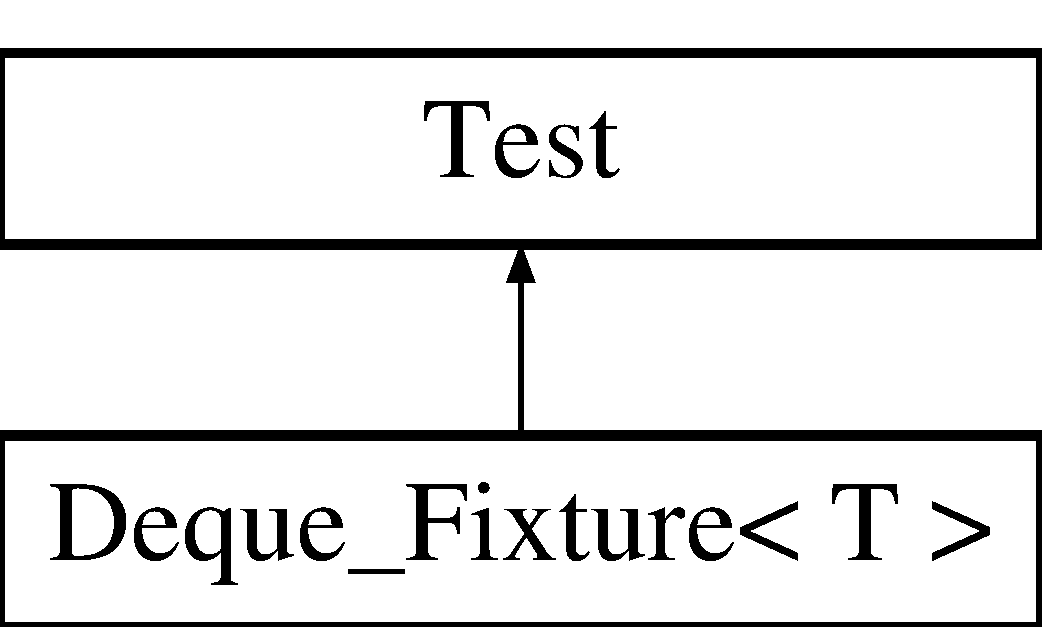
\includegraphics[height=2.000000cm]{structDeque__Fixture}
\end{center}
\end{figure}
\subsection*{Public Types}
\begin{DoxyCompactItemize}
\item 
typedef T \hyperlink{structDeque__Fixture_aff55aebc9f3732e55b5e9afae069a6e7}{deque\-\_\-type}
\item 
typedef deque\-\_\-type\-::value\-\_\-type \hyperlink{structDeque__Fixture_ad3f31d2190bcef2a8809aae173c159e9}{value\-\_\-type}
\end{DoxyCompactItemize}


\subsection{Member Typedef Documentation}
\hypertarget{structDeque__Fixture_aff55aebc9f3732e55b5e9afae069a6e7}{\index{Deque\-\_\-\-Fixture@{Deque\-\_\-\-Fixture}!deque\-\_\-type@{deque\-\_\-type}}
\index{deque\-\_\-type@{deque\-\_\-type}!Deque_Fixture@{Deque\-\_\-\-Fixture}}
\subsubsection[{deque\-\_\-type}]{\setlength{\rightskip}{0pt plus 5cm}template$<$typename T $>$ typedef T {\bf Deque\-\_\-\-Fixture}$<$ T $>$\-::{\bf deque\-\_\-type}}}\label{structDeque__Fixture_aff55aebc9f3732e55b5e9afae069a6e7}
\hypertarget{structDeque__Fixture_ad3f31d2190bcef2a8809aae173c159e9}{\index{Deque\-\_\-\-Fixture@{Deque\-\_\-\-Fixture}!value\-\_\-type@{value\-\_\-type}}
\index{value\-\_\-type@{value\-\_\-type}!Deque_Fixture@{Deque\-\_\-\-Fixture}}
\subsubsection[{value\-\_\-type}]{\setlength{\rightskip}{0pt plus 5cm}template$<$typename T $>$ typedef deque\-\_\-type\-::value\-\_\-type {\bf Deque\-\_\-\-Fixture}$<$ T $>$\-::{\bf value\-\_\-type}}}\label{structDeque__Fixture_ad3f31d2190bcef2a8809aae173c159e9}


The documentation for this struct was generated from the following file\-:\begin{DoxyCompactItemize}
\item 
\hyperlink{TestDeque_8c_09_09}{Test\-Deque.\-c++}\end{DoxyCompactItemize}

\hypertarget{classmy__deque_1_1iterator}{\section{my\-\_\-deque$<$ T, A $>$\-:\-:iterator Class Reference}
\label{classmy__deque_1_1iterator}\index{my\-\_\-deque$<$ T, A $>$\-::iterator@{my\-\_\-deque$<$ T, A $>$\-::iterator}}
}


{\ttfamily \#include $<$Deque.\-h$>$}

\subsection*{Public Types}
\begin{DoxyCompactItemize}
\item 
typedef \\*
std\-::bidirectional\-\_\-iterator\-\_\-tag \hyperlink{classmy__deque_1_1iterator_a0479a0f5fbb1adddafb03cd2c9aaef53}{iterator\-\_\-category}
\item 
typedef \hyperlink{classmy__deque_ae9c156c405acc57623a4601ce755596f}{my\-\_\-deque\-::value\-\_\-type} \hyperlink{classmy__deque_1_1iterator_ac6392e82698893d1802ef0407bd36794}{value\-\_\-type}
\item 
typedef \hyperlink{classmy__deque_ac85676cb2492fbc9bbc6f1a30e9d3c73}{my\-\_\-deque\-::difference\-\_\-type} \hyperlink{classmy__deque_1_1iterator_ac5f62e8566ad92478931c2abd9ac6596}{difference\-\_\-type}
\item 
typedef \hyperlink{classmy__deque_a58e82fc365a3b086367479515e1515be}{my\-\_\-deque\-::pointer} \hyperlink{classmy__deque_1_1iterator_add0e1ed49072422b5aa0ef52303fb86e}{pointer}
\item 
typedef \hyperlink{classmy__deque_a4c34c14f397b7676445b37c87003116b}{my\-\_\-deque\-::reference} \hyperlink{classmy__deque_1_1iterator_ae165ee997a9e18330c593789e9899e57}{reference}
\item 
typedef \hyperlink{classmy__deque_a61e5e5317fe72a381ce4d45f09544b02}{my\-\_\-deque\-::size\-\_\-type} \hyperlink{classmy__deque_1_1iterator_a23ff400617b1c6b42ff3f67fb318d19d}{size\-\_\-type}
\end{DoxyCompactItemize}
\subsection*{Public Member Functions}
\begin{DoxyCompactItemize}
\item 
\hyperlink{classmy__deque_1_1iterator_af810e94f668ed8bf7fa5be5788c79099}{iterator} (\hyperlink{classmy__deque}{my\-\_\-deque} $\ast$myd, \hyperlink{classmy__deque_1_1iterator_a23ff400617b1c6b42ff3f67fb318d19d}{size\-\_\-type} inner\-\_\-index, \hyperlink{classmy__deque_1_1iterator_a23ff400617b1c6b42ff3f67fb318d19d}{size\-\_\-type} outer\-\_\-index)
\item 
\hyperlink{classmy__deque_1_1iterator_ae165ee997a9e18330c593789e9899e57}{reference} \hyperlink{classmy__deque_1_1iterator_a12632f02814bba64ca79f42edc0e1497}{operator$\ast$} () const 
\item 
\hyperlink{classmy__deque_1_1iterator_add0e1ed49072422b5aa0ef52303fb86e}{pointer} \hyperlink{classmy__deque_1_1iterator_a064f5b1faf5a72113083425133de9a41}{operator-\/$>$} () const 
\item 
\hyperlink{classmy__deque_1_1iterator}{iterator} \& \hyperlink{classmy__deque_1_1iterator_ab2a00619614e204eedb184112a56016e}{operator++} ()
\item 
\hyperlink{classmy__deque_1_1iterator}{iterator} \hyperlink{classmy__deque_1_1iterator_a57f6ac4aef7215ca67b6e05eeda29ee4}{operator++} (int)
\item 
\hyperlink{classmy__deque_1_1iterator}{iterator} \& \hyperlink{classmy__deque_1_1iterator_a278cab96c03498e55ba1aa4e05f1538e}{operator-\/-\/} ()
\item 
\hyperlink{classmy__deque_1_1iterator}{iterator} \hyperlink{classmy__deque_1_1iterator_a5bef4b6332aecf7dcda57cee9a1fdc70}{operator-\/-\/} (int)
\item 
\hyperlink{classmy__deque_1_1iterator}{iterator} \& \hyperlink{classmy__deque_1_1iterator_ad17b4f6e8be4d8242ad4572d62beff82}{operator+=} (\hyperlink{classmy__deque_1_1iterator_ac5f62e8566ad92478931c2abd9ac6596}{difference\-\_\-type} d)
\item 
\hyperlink{classmy__deque_1_1iterator}{iterator} \& \hyperlink{classmy__deque_1_1iterator_a13c056d48543734a23a9de09fd652868}{operator-\/=} (\hyperlink{classmy__deque_1_1iterator_ac5f62e8566ad92478931c2abd9ac6596}{difference\-\_\-type} d)
\end{DoxyCompactItemize}
\subsection*{Private Member Functions}
\begin{DoxyCompactItemize}
\item 
bool \hyperlink{classmy__deque_1_1iterator_a4e56b174bbf8c52c58e2f3934be7fc75}{valid} () const 
\end{DoxyCompactItemize}
\subsection*{Private Attributes}
\begin{DoxyCompactItemize}
\item 
\hyperlink{classmy__deque}{my\-\_\-deque} $\ast$ \hyperlink{classmy__deque_1_1iterator_a00058b213271faa0b36b8e8137d015f1}{dq}
\item 
\hyperlink{classmy__deque_1_1iterator_a23ff400617b1c6b42ff3f67fb318d19d}{size\-\_\-type} \hyperlink{classmy__deque_1_1iterator_a418fb5071b8437c9a0259ad1cb19aeb8}{\-\_\-front\-\_\-outer\-\_\-index}
\item 
\hyperlink{classmy__deque_1_1iterator_a23ff400617b1c6b42ff3f67fb318d19d}{size\-\_\-type} \hyperlink{classmy__deque_1_1iterator_a384bcfc2da11135412c0211261464f95}{\-\_\-front\-\_\-inner\-\_\-index}
\end{DoxyCompactItemize}
\subsection*{Friends}
\begin{DoxyCompactItemize}
\item 
bool \hyperlink{classmy__deque_1_1iterator_a27d0df37bd079bf4e62faa0b468b060c}{operator==} (const \hyperlink{classmy__deque_1_1iterator}{iterator} \&lhs, const \hyperlink{classmy__deque_1_1iterator}{iterator} \&rhs)
\item 
bool \hyperlink{classmy__deque_1_1iterator_aad2b3926ed1e2db6f22ca3117766181b}{operator!=} (const \hyperlink{classmy__deque_1_1iterator}{iterator} \&lhs, const \hyperlink{classmy__deque_1_1iterator}{iterator} \&rhs)
\item 
\hyperlink{classmy__deque_1_1iterator}{iterator} \hyperlink{classmy__deque_1_1iterator_aaf128f38c16b5a8284f51a9c69f6fd77}{operator+} (\hyperlink{classmy__deque_1_1iterator}{iterator} lhs, \hyperlink{classmy__deque_1_1iterator_ac5f62e8566ad92478931c2abd9ac6596}{difference\-\_\-type} rhs)
\item 
\hyperlink{classmy__deque_1_1iterator}{iterator} \hyperlink{classmy__deque_1_1iterator_ab8892736ecb2ffe5f6b9ac9b9dbb60c0}{operator-\/} (\hyperlink{classmy__deque_1_1iterator}{iterator} lhs, \hyperlink{classmy__deque_1_1iterator_ac5f62e8566ad92478931c2abd9ac6596}{difference\-\_\-type} rhs)
\end{DoxyCompactItemize}


\subsection{Member Typedef Documentation}
\hypertarget{classmy__deque_1_1iterator_ac5f62e8566ad92478931c2abd9ac6596}{\index{my\-\_\-deque\-::iterator@{my\-\_\-deque\-::iterator}!difference\-\_\-type@{difference\-\_\-type}}
\index{difference\-\_\-type@{difference\-\_\-type}!my_deque::iterator@{my\-\_\-deque\-::iterator}}
\subsubsection[{difference\-\_\-type}]{\setlength{\rightskip}{0pt plus 5cm}template$<$typename T , typename A  = std\-::allocator$<$\-T$>$$>$ typedef {\bf my\-\_\-deque\-::difference\-\_\-type} {\bf my\-\_\-deque}$<$ T, A $>$\-::{\bf iterator\-::difference\-\_\-type}}}\label{classmy__deque_1_1iterator_ac5f62e8566ad92478931c2abd9ac6596}
\hypertarget{classmy__deque_1_1iterator_a0479a0f5fbb1adddafb03cd2c9aaef53}{\index{my\-\_\-deque\-::iterator@{my\-\_\-deque\-::iterator}!iterator\-\_\-category@{iterator\-\_\-category}}
\index{iterator\-\_\-category@{iterator\-\_\-category}!my_deque::iterator@{my\-\_\-deque\-::iterator}}
\subsubsection[{iterator\-\_\-category}]{\setlength{\rightskip}{0pt plus 5cm}template$<$typename T , typename A  = std\-::allocator$<$\-T$>$$>$ typedef std\-::bidirectional\-\_\-iterator\-\_\-tag {\bf my\-\_\-deque}$<$ T, A $>$\-::{\bf iterator\-::iterator\-\_\-category}}}\label{classmy__deque_1_1iterator_a0479a0f5fbb1adddafb03cd2c9aaef53}
\hypertarget{classmy__deque_1_1iterator_add0e1ed49072422b5aa0ef52303fb86e}{\index{my\-\_\-deque\-::iterator@{my\-\_\-deque\-::iterator}!pointer@{pointer}}
\index{pointer@{pointer}!my_deque::iterator@{my\-\_\-deque\-::iterator}}
\subsubsection[{pointer}]{\setlength{\rightskip}{0pt plus 5cm}template$<$typename T , typename A  = std\-::allocator$<$\-T$>$$>$ typedef {\bf my\-\_\-deque\-::pointer} {\bf my\-\_\-deque}$<$ T, A $>$\-::{\bf iterator\-::pointer}}}\label{classmy__deque_1_1iterator_add0e1ed49072422b5aa0ef52303fb86e}
\hypertarget{classmy__deque_1_1iterator_ae165ee997a9e18330c593789e9899e57}{\index{my\-\_\-deque\-::iterator@{my\-\_\-deque\-::iterator}!reference@{reference}}
\index{reference@{reference}!my_deque::iterator@{my\-\_\-deque\-::iterator}}
\subsubsection[{reference}]{\setlength{\rightskip}{0pt plus 5cm}template$<$typename T , typename A  = std\-::allocator$<$\-T$>$$>$ typedef {\bf my\-\_\-deque\-::reference} {\bf my\-\_\-deque}$<$ T, A $>$\-::{\bf iterator\-::reference}}}\label{classmy__deque_1_1iterator_ae165ee997a9e18330c593789e9899e57}
\hypertarget{classmy__deque_1_1iterator_a23ff400617b1c6b42ff3f67fb318d19d}{\index{my\-\_\-deque\-::iterator@{my\-\_\-deque\-::iterator}!size\-\_\-type@{size\-\_\-type}}
\index{size\-\_\-type@{size\-\_\-type}!my_deque::iterator@{my\-\_\-deque\-::iterator}}
\subsubsection[{size\-\_\-type}]{\setlength{\rightskip}{0pt plus 5cm}template$<$typename T , typename A  = std\-::allocator$<$\-T$>$$>$ typedef {\bf my\-\_\-deque\-::size\-\_\-type} {\bf my\-\_\-deque}$<$ T, A $>$\-::{\bf iterator\-::size\-\_\-type}}}\label{classmy__deque_1_1iterator_a23ff400617b1c6b42ff3f67fb318d19d}
\hypertarget{classmy__deque_1_1iterator_ac6392e82698893d1802ef0407bd36794}{\index{my\-\_\-deque\-::iterator@{my\-\_\-deque\-::iterator}!value\-\_\-type@{value\-\_\-type}}
\index{value\-\_\-type@{value\-\_\-type}!my_deque::iterator@{my\-\_\-deque\-::iterator}}
\subsubsection[{value\-\_\-type}]{\setlength{\rightskip}{0pt plus 5cm}template$<$typename T , typename A  = std\-::allocator$<$\-T$>$$>$ typedef {\bf my\-\_\-deque\-::value\-\_\-type} {\bf my\-\_\-deque}$<$ T, A $>$\-::{\bf iterator\-::value\-\_\-type}}}\label{classmy__deque_1_1iterator_ac6392e82698893d1802ef0407bd36794}


\subsection{Constructor \& Destructor Documentation}
\hypertarget{classmy__deque_1_1iterator_af810e94f668ed8bf7fa5be5788c79099}{\index{my\-\_\-deque\-::iterator@{my\-\_\-deque\-::iterator}!iterator@{iterator}}
\index{iterator@{iterator}!my_deque::iterator@{my\-\_\-deque\-::iterator}}
\subsubsection[{iterator}]{\setlength{\rightskip}{0pt plus 5cm}template$<$typename T , typename A  = std\-::allocator$<$\-T$>$$>$ {\bf my\-\_\-deque}$<$ T, A $>$\-::iterator\-::iterator (
\begin{DoxyParamCaption}
\item[{{\bf my\-\_\-deque} $\ast$}]{myd, }
\item[{{\bf size\-\_\-type}}]{inner\-\_\-index, }
\item[{{\bf size\-\_\-type}}]{outer\-\_\-index}
\end{DoxyParamCaption}
)\hspace{0.3cm}{\ttfamily [inline]}}}\label{classmy__deque_1_1iterator_af810e94f668ed8bf7fa5be5788c79099}
iterator constructor 

\subsection{Member Function Documentation}
\hypertarget{classmy__deque_1_1iterator_a12632f02814bba64ca79f42edc0e1497}{\index{my\-\_\-deque\-::iterator@{my\-\_\-deque\-::iterator}!operator$\ast$@{operator$\ast$}}
\index{operator$\ast$@{operator$\ast$}!my_deque::iterator@{my\-\_\-deque\-::iterator}}
\subsubsection[{operator$\ast$}]{\setlength{\rightskip}{0pt plus 5cm}template$<$typename T , typename A  = std\-::allocator$<$\-T$>$$>$ {\bf reference} {\bf my\-\_\-deque}$<$ T, A $>$\-::iterator\-::operator$\ast$ (
\begin{DoxyParamCaption}
{}
\end{DoxyParamCaption}
) const\hspace{0.3cm}{\ttfamily [inline]}}}\label{classmy__deque_1_1iterator_a12632f02814bba64ca79f42edc0e1497}
grabs value at the iterator location \hypertarget{classmy__deque_1_1iterator_ab2a00619614e204eedb184112a56016e}{\index{my\-\_\-deque\-::iterator@{my\-\_\-deque\-::iterator}!operator++@{operator++}}
\index{operator++@{operator++}!my_deque::iterator@{my\-\_\-deque\-::iterator}}
\subsubsection[{operator++}]{\setlength{\rightskip}{0pt plus 5cm}template$<$typename T , typename A  = std\-::allocator$<$\-T$>$$>$ {\bf iterator}\& {\bf my\-\_\-deque}$<$ T, A $>$\-::iterator\-::operator++ (
\begin{DoxyParamCaption}
{}
\end{DoxyParamCaption}
)\hspace{0.3cm}{\ttfamily [inline]}}}\label{classmy__deque_1_1iterator_ab2a00619614e204eedb184112a56016e}
iterator incrment pre \hypertarget{classmy__deque_1_1iterator_a57f6ac4aef7215ca67b6e05eeda29ee4}{\index{my\-\_\-deque\-::iterator@{my\-\_\-deque\-::iterator}!operator++@{operator++}}
\index{operator++@{operator++}!my_deque::iterator@{my\-\_\-deque\-::iterator}}
\subsubsection[{operator++}]{\setlength{\rightskip}{0pt plus 5cm}template$<$typename T , typename A  = std\-::allocator$<$\-T$>$$>$ {\bf iterator} {\bf my\-\_\-deque}$<$ T, A $>$\-::iterator\-::operator++ (
\begin{DoxyParamCaption}
\item[{int}]{}
\end{DoxyParamCaption}
)\hspace{0.3cm}{\ttfamily [inline]}}}\label{classmy__deque_1_1iterator_a57f6ac4aef7215ca67b6e05eeda29ee4}
iterator increment post \hypertarget{classmy__deque_1_1iterator_ad17b4f6e8be4d8242ad4572d62beff82}{\index{my\-\_\-deque\-::iterator@{my\-\_\-deque\-::iterator}!operator+=@{operator+=}}
\index{operator+=@{operator+=}!my_deque::iterator@{my\-\_\-deque\-::iterator}}
\subsubsection[{operator+=}]{\setlength{\rightskip}{0pt plus 5cm}template$<$typename T , typename A  = std\-::allocator$<$\-T$>$$>$ {\bf iterator}\& {\bf my\-\_\-deque}$<$ T, A $>$\-::iterator\-::operator+= (
\begin{DoxyParamCaption}
\item[{{\bf difference\-\_\-type}}]{d}
\end{DoxyParamCaption}
)\hspace{0.3cm}{\ttfamily [inline]}}}\label{classmy__deque_1_1iterator_ad17b4f6e8be4d8242ad4572d62beff82}
iterator += \hypertarget{classmy__deque_1_1iterator_a278cab96c03498e55ba1aa4e05f1538e}{\index{my\-\_\-deque\-::iterator@{my\-\_\-deque\-::iterator}!operator-\/-\/@{operator-\/-\/}}
\index{operator-\/-\/@{operator-\/-\/}!my_deque::iterator@{my\-\_\-deque\-::iterator}}
\subsubsection[{operator-\/-\/}]{\setlength{\rightskip}{0pt plus 5cm}template$<$typename T , typename A  = std\-::allocator$<$\-T$>$$>$ {\bf iterator}\& {\bf my\-\_\-deque}$<$ T, A $>$\-::iterator\-::operator-\/-\/ (
\begin{DoxyParamCaption}
{}
\end{DoxyParamCaption}
)\hspace{0.3cm}{\ttfamily [inline]}}}\label{classmy__deque_1_1iterator_a278cab96c03498e55ba1aa4e05f1538e}
iterator pre decrement \hypertarget{classmy__deque_1_1iterator_a5bef4b6332aecf7dcda57cee9a1fdc70}{\index{my\-\_\-deque\-::iterator@{my\-\_\-deque\-::iterator}!operator-\/-\/@{operator-\/-\/}}
\index{operator-\/-\/@{operator-\/-\/}!my_deque::iterator@{my\-\_\-deque\-::iterator}}
\subsubsection[{operator-\/-\/}]{\setlength{\rightskip}{0pt plus 5cm}template$<$typename T , typename A  = std\-::allocator$<$\-T$>$$>$ {\bf iterator} {\bf my\-\_\-deque}$<$ T, A $>$\-::iterator\-::operator-\/-\/ (
\begin{DoxyParamCaption}
\item[{int}]{}
\end{DoxyParamCaption}
)\hspace{0.3cm}{\ttfamily [inline]}}}\label{classmy__deque_1_1iterator_a5bef4b6332aecf7dcda57cee9a1fdc70}
iterator post decrement \hypertarget{classmy__deque_1_1iterator_a13c056d48543734a23a9de09fd652868}{\index{my\-\_\-deque\-::iterator@{my\-\_\-deque\-::iterator}!operator-\/=@{operator-\/=}}
\index{operator-\/=@{operator-\/=}!my_deque::iterator@{my\-\_\-deque\-::iterator}}
\subsubsection[{operator-\/=}]{\setlength{\rightskip}{0pt plus 5cm}template$<$typename T , typename A  = std\-::allocator$<$\-T$>$$>$ {\bf iterator}\& {\bf my\-\_\-deque}$<$ T, A $>$\-::iterator\-::operator-\/= (
\begin{DoxyParamCaption}
\item[{{\bf difference\-\_\-type}}]{d}
\end{DoxyParamCaption}
)\hspace{0.3cm}{\ttfamily [inline]}}}\label{classmy__deque_1_1iterator_a13c056d48543734a23a9de09fd652868}
iterator -\/= \hypertarget{classmy__deque_1_1iterator_a064f5b1faf5a72113083425133de9a41}{\index{my\-\_\-deque\-::iterator@{my\-\_\-deque\-::iterator}!operator-\/$>$@{operator-\/$>$}}
\index{operator-\/$>$@{operator-\/$>$}!my_deque::iterator@{my\-\_\-deque\-::iterator}}
\subsubsection[{operator-\/$>$}]{\setlength{\rightskip}{0pt plus 5cm}template$<$typename T , typename A  = std\-::allocator$<$\-T$>$$>$ {\bf pointer} {\bf my\-\_\-deque}$<$ T, A $>$\-::iterator\-::operator-\/$>$ (
\begin{DoxyParamCaption}
{}
\end{DoxyParamCaption}
) const\hspace{0.3cm}{\ttfamily [inline]}}}\label{classmy__deque_1_1iterator_a064f5b1faf5a72113083425133de9a41}
value operator \hypertarget{classmy__deque_1_1iterator_a4e56b174bbf8c52c58e2f3934be7fc75}{\index{my\-\_\-deque\-::iterator@{my\-\_\-deque\-::iterator}!valid@{valid}}
\index{valid@{valid}!my_deque::iterator@{my\-\_\-deque\-::iterator}}
\subsubsection[{valid}]{\setlength{\rightskip}{0pt plus 5cm}template$<$typename T , typename A  = std\-::allocator$<$\-T$>$$>$ bool {\bf my\-\_\-deque}$<$ T, A $>$\-::iterator\-::valid (
\begin{DoxyParamCaption}
{}
\end{DoxyParamCaption}
) const\hspace{0.3cm}{\ttfamily [inline]}, {\ttfamily [private]}}}\label{classmy__deque_1_1iterator_a4e56b174bbf8c52c58e2f3934be7fc75}


\subsection{Friends And Related Function Documentation}
\hypertarget{classmy__deque_1_1iterator_aad2b3926ed1e2db6f22ca3117766181b}{\index{my\-\_\-deque\-::iterator@{my\-\_\-deque\-::iterator}!operator!=@{operator!=}}
\index{operator!=@{operator!=}!my_deque::iterator@{my\-\_\-deque\-::iterator}}
\subsubsection[{operator!=}]{\setlength{\rightskip}{0pt plus 5cm}template$<$typename T , typename A  = std\-::allocator$<$\-T$>$$>$ bool operator!= (
\begin{DoxyParamCaption}
\item[{const {\bf iterator} \&}]{lhs, }
\item[{const {\bf iterator} \&}]{rhs}
\end{DoxyParamCaption}
)\hspace{0.3cm}{\ttfamily [friend]}}}\label{classmy__deque_1_1iterator_aad2b3926ed1e2db6f22ca3117766181b}
$<$your documentation$>$=\char`\"{}\char`\"{}$>$ \hypertarget{classmy__deque_1_1iterator_aaf128f38c16b5a8284f51a9c69f6fd77}{\index{my\-\_\-deque\-::iterator@{my\-\_\-deque\-::iterator}!operator+@{operator+}}
\index{operator+@{operator+}!my_deque::iterator@{my\-\_\-deque\-::iterator}}
\subsubsection[{operator+}]{\setlength{\rightskip}{0pt plus 5cm}template$<$typename T , typename A  = std\-::allocator$<$\-T$>$$>$ {\bf iterator} operator+ (
\begin{DoxyParamCaption}
\item[{{\bf iterator}}]{lhs, }
\item[{{\bf difference\-\_\-type}}]{rhs}
\end{DoxyParamCaption}
)\hspace{0.3cm}{\ttfamily [friend]}}}\label{classmy__deque_1_1iterator_aaf128f38c16b5a8284f51a9c69f6fd77}
$<$your documentation$>$=\char`\"{}\char`\"{}$>$ \hypertarget{classmy__deque_1_1iterator_ab8892736ecb2ffe5f6b9ac9b9dbb60c0}{\index{my\-\_\-deque\-::iterator@{my\-\_\-deque\-::iterator}!operator-\/@{operator-\/}}
\index{operator-\/@{operator-\/}!my_deque::iterator@{my\-\_\-deque\-::iterator}}
\subsubsection[{operator-\/}]{\setlength{\rightskip}{0pt plus 5cm}template$<$typename T , typename A  = std\-::allocator$<$\-T$>$$>$ {\bf iterator} operator-\/ (
\begin{DoxyParamCaption}
\item[{{\bf iterator}}]{lhs, }
\item[{{\bf difference\-\_\-type}}]{rhs}
\end{DoxyParamCaption}
)\hspace{0.3cm}{\ttfamily [friend]}}}\label{classmy__deque_1_1iterator_ab8892736ecb2ffe5f6b9ac9b9dbb60c0}
$<$your documentation$>$=\char`\"{}\char`\"{}$>$ \hypertarget{classmy__deque_1_1iterator_a27d0df37bd079bf4e62faa0b468b060c}{\index{my\-\_\-deque\-::iterator@{my\-\_\-deque\-::iterator}!operator==@{operator==}}
\index{operator==@{operator==}!my_deque::iterator@{my\-\_\-deque\-::iterator}}
\subsubsection[{operator==}]{\setlength{\rightskip}{0pt plus 5cm}template$<$typename T , typename A  = std\-::allocator$<$\-T$>$$>$ bool operator== (
\begin{DoxyParamCaption}
\item[{const {\bf iterator} \&}]{lhs, }
\item[{const {\bf iterator} \&}]{rhs}
\end{DoxyParamCaption}
)\hspace{0.3cm}{\ttfamily [friend]}}}\label{classmy__deque_1_1iterator_a27d0df37bd079bf4e62faa0b468b060c}
$<$your documentation$>$=\char`\"{}\char`\"{}$>$ 

\subsection{Member Data Documentation}
\hypertarget{classmy__deque_1_1iterator_a384bcfc2da11135412c0211261464f95}{\index{my\-\_\-deque\-::iterator@{my\-\_\-deque\-::iterator}!\-\_\-front\-\_\-inner\-\_\-index@{\-\_\-front\-\_\-inner\-\_\-index}}
\index{\-\_\-front\-\_\-inner\-\_\-index@{\-\_\-front\-\_\-inner\-\_\-index}!my_deque::iterator@{my\-\_\-deque\-::iterator}}
\subsubsection[{\-\_\-front\-\_\-inner\-\_\-index}]{\setlength{\rightskip}{0pt plus 5cm}template$<$typename T , typename A  = std\-::allocator$<$\-T$>$$>$ {\bf size\-\_\-type} {\bf my\-\_\-deque}$<$ T, A $>$\-::iterator\-::\-\_\-front\-\_\-inner\-\_\-index\hspace{0.3cm}{\ttfamily [private]}}}\label{classmy__deque_1_1iterator_a384bcfc2da11135412c0211261464f95}
\hypertarget{classmy__deque_1_1iterator_a418fb5071b8437c9a0259ad1cb19aeb8}{\index{my\-\_\-deque\-::iterator@{my\-\_\-deque\-::iterator}!\-\_\-front\-\_\-outer\-\_\-index@{\-\_\-front\-\_\-outer\-\_\-index}}
\index{\-\_\-front\-\_\-outer\-\_\-index@{\-\_\-front\-\_\-outer\-\_\-index}!my_deque::iterator@{my\-\_\-deque\-::iterator}}
\subsubsection[{\-\_\-front\-\_\-outer\-\_\-index}]{\setlength{\rightskip}{0pt plus 5cm}template$<$typename T , typename A  = std\-::allocator$<$\-T$>$$>$ {\bf size\-\_\-type} {\bf my\-\_\-deque}$<$ T, A $>$\-::iterator\-::\-\_\-front\-\_\-outer\-\_\-index\hspace{0.3cm}{\ttfamily [private]}}}\label{classmy__deque_1_1iterator_a418fb5071b8437c9a0259ad1cb19aeb8}
\hypertarget{classmy__deque_1_1iterator_a00058b213271faa0b36b8e8137d015f1}{\index{my\-\_\-deque\-::iterator@{my\-\_\-deque\-::iterator}!dq@{dq}}
\index{dq@{dq}!my_deque::iterator@{my\-\_\-deque\-::iterator}}
\subsubsection[{dq}]{\setlength{\rightskip}{0pt plus 5cm}template$<$typename T , typename A  = std\-::allocator$<$\-T$>$$>$ {\bf my\-\_\-deque}$\ast$ {\bf my\-\_\-deque}$<$ T, A $>$\-::iterator\-::dq\hspace{0.3cm}{\ttfamily [private]}}}\label{classmy__deque_1_1iterator_a00058b213271faa0b36b8e8137d015f1}


The documentation for this class was generated from the following file\-:\begin{DoxyCompactItemize}
\item 
\hyperlink{Deque_8h}{Deque.\-h}\end{DoxyCompactItemize}

\hypertarget{classmy__deque}{\section{my\-\_\-deque$<$ T, A $>$ Class Template Reference}
\label{classmy__deque}\index{my\-\_\-deque$<$ T, A $>$@{my\-\_\-deque$<$ T, A $>$}}
}


{\ttfamily \#include $<$Deque.\-h$>$}

\subsection*{Classes}
\begin{DoxyCompactItemize}
\item 
class \hyperlink{classmy__deque_1_1const__iterator}{const\-\_\-iterator}
\item 
class \hyperlink{classmy__deque_1_1iterator}{iterator}
\end{DoxyCompactItemize}
\subsection*{Public Types}
\begin{DoxyCompactItemize}
\item 
typedef A \hyperlink{classmy__deque_a34236f0fef930decd11dc683f40a38be}{allocator\-\_\-type}
\item 
typedef allocator\-\_\-type\-::value\-\_\-type \hyperlink{classmy__deque_ae9c156c405acc57623a4601ce755596f}{value\-\_\-type}
\item 
typedef allocator\-\_\-type\-::size\-\_\-type \hyperlink{classmy__deque_a61e5e5317fe72a381ce4d45f09544b02}{size\-\_\-type}
\item 
typedef \\*
allocator\-\_\-type\-::difference\-\_\-type \hyperlink{classmy__deque_ac85676cb2492fbc9bbc6f1a30e9d3c73}{difference\-\_\-type}
\item 
typedef allocator\-\_\-type\-::pointer \hyperlink{classmy__deque_a58e82fc365a3b086367479515e1515be}{pointer}
\item 
typedef \\*
allocator\-\_\-type\-::const\-\_\-pointer \hyperlink{classmy__deque_a8fea5edeb2b2cf3dd1246dc3abf9b71b}{const\-\_\-pointer}
\item 
typedef allocator\-\_\-type\-::reference \hyperlink{classmy__deque_a4c34c14f397b7676445b37c87003116b}{reference}
\item 
typedef \\*
allocator\-\_\-type\-::const\-\_\-reference \hyperlink{classmy__deque_ad50d8b378580088cf77fa43f0640e49c}{const\-\_\-reference}
\item 
typedef A\-::template rebind\\*
$<$ \hyperlink{classmy__deque_a58e82fc365a3b086367479515e1515be}{pointer} $>$\-::other \hyperlink{classmy__deque_a1a55c016646bba79086d90d3cccde143}{B}
\end{DoxyCompactItemize}
\subsection*{Public Member Functions}
\begin{DoxyCompactItemize}
\item 
\hyperlink{classmy__deque_ad2ac9d80048c55fcc045d2861c73aa1a}{my\-\_\-deque} (const \hyperlink{classmy__deque_a34236f0fef930decd11dc683f40a38be}{allocator\-\_\-type} \&a=\hyperlink{classmy__deque_a34236f0fef930decd11dc683f40a38be}{allocator\-\_\-type}())
\item 
\hyperlink{classmy__deque_aeaf4c625438497a7cd6a670da6c2c08b}{my\-\_\-deque} (\hyperlink{classmy__deque_a61e5e5317fe72a381ce4d45f09544b02}{size\-\_\-type} s, \hyperlink{classmy__deque_ad50d8b378580088cf77fa43f0640e49c}{const\-\_\-reference} v=\hyperlink{classmy__deque_ae9c156c405acc57623a4601ce755596f}{value\-\_\-type}(), const \hyperlink{classmy__deque_a34236f0fef930decd11dc683f40a38be}{allocator\-\_\-type} \&a=\hyperlink{classmy__deque_a34236f0fef930decd11dc683f40a38be}{allocator\-\_\-type}())
\item 
\hyperlink{classmy__deque_a59015bc46e6096555d631d69dc8fd7e7}{my\-\_\-deque} (const \hyperlink{classmy__deque}{my\-\_\-deque} \&that)
\item 
\hyperlink{classmy__deque_ae22194ee436865a59a7475c339a9c1ca}{$\sim$my\-\_\-deque} ()
\item 
\hyperlink{classmy__deque}{my\-\_\-deque} \& \hyperlink{classmy__deque_aaa103f2058854bb98e500de6305b1564}{operator=} (const \hyperlink{classmy__deque}{my\-\_\-deque} \&rhs)
\item 
\hyperlink{classmy__deque_a4c34c14f397b7676445b37c87003116b}{reference} \hyperlink{classmy__deque_a489b77decf4d424f43092e194d69444f}{operator\mbox{[}$\,$\mbox{]}} (\hyperlink{classmy__deque_a61e5e5317fe72a381ce4d45f09544b02}{size\-\_\-type} index)
\item 
\hyperlink{classmy__deque_ad50d8b378580088cf77fa43f0640e49c}{const\-\_\-reference} \hyperlink{classmy__deque_ad79fcd9e94dfc5566e1cd0ce606cf208}{operator\mbox{[}$\,$\mbox{]}} (\hyperlink{classmy__deque_a61e5e5317fe72a381ce4d45f09544b02}{size\-\_\-type} index) const 
\item 
\hyperlink{classmy__deque_a4c34c14f397b7676445b37c87003116b}{reference} \hyperlink{classmy__deque_a75106748e6ff8735e40560e7335bd500}{at} (\hyperlink{classmy__deque_a61e5e5317fe72a381ce4d45f09544b02}{size\-\_\-type} index)
\item 
\hyperlink{classmy__deque_ad50d8b378580088cf77fa43f0640e49c}{const\-\_\-reference} \hyperlink{classmy__deque_a9642816a10e6a6ee1f8a5367987b8ee8}{at} (\hyperlink{classmy__deque_a61e5e5317fe72a381ce4d45f09544b02}{size\-\_\-type} index) const 
\item 
\hyperlink{classmy__deque_a4c34c14f397b7676445b37c87003116b}{reference} \hyperlink{classmy__deque_a1d9aadb5bedc29da86d4323587cd5e4d}{back} ()
\item 
\hyperlink{classmy__deque_ad50d8b378580088cf77fa43f0640e49c}{const\-\_\-reference} \hyperlink{classmy__deque_ac273f9574a95af619b9f0dcc0d2e89d0}{back} () const 
\item 
\hyperlink{classmy__deque_1_1iterator}{iterator} \hyperlink{classmy__deque_aef8cac69d47cb1c274896b82ba8f453a}{begin} ()
\item 
\hyperlink{classmy__deque_1_1const__iterator}{const\-\_\-iterator} \hyperlink{classmy__deque_a8612539eff4ee446f85ffb30abf91a69}{begin} () const 
\item 
void \hyperlink{classmy__deque_aa29f90c63cde532f5fc169e8e66b514c}{clear} ()
\item 
bool \hyperlink{classmy__deque_a2b4f029c47afbdbf057639c5a6816d6c}{empty} () const 
\item 
\hyperlink{classmy__deque_1_1iterator}{iterator} \hyperlink{classmy__deque_a2576ee71790ebe55ac4200c506540bb5}{end} ()
\item 
\hyperlink{classmy__deque_1_1const__iterator}{const\-\_\-iterator} \hyperlink{classmy__deque_af465c3f8483634e4e656d90f8d0d88fb}{end} () const 
\item 
\hyperlink{classmy__deque_1_1iterator}{iterator} \hyperlink{classmy__deque_a68328ee9d14996c56ccac5e9981741d5}{erase} (\hyperlink{classmy__deque_1_1iterator}{iterator} i)
\item 
\hyperlink{classmy__deque_a4c34c14f397b7676445b37c87003116b}{reference} \hyperlink{classmy__deque_a0eae28af0ffdd813d1f94f57d393fdf8}{front} ()
\item 
\hyperlink{classmy__deque_ad50d8b378580088cf77fa43f0640e49c}{const\-\_\-reference} \hyperlink{classmy__deque_a0f1239043b7339b8237a0c8bc663be6b}{front} () const 
\item 
\hyperlink{classmy__deque_1_1iterator}{iterator} \hyperlink{classmy__deque_af5dee5eeded9eb5392b09731cc126d76}{insert} (\hyperlink{classmy__deque_1_1iterator}{iterator} i, \hyperlink{classmy__deque_ad50d8b378580088cf77fa43f0640e49c}{const\-\_\-reference} v)
\item 
void \hyperlink{classmy__deque_a63cc9691ee90701693e948246311c498}{pop\-\_\-back} ()
\item 
void \hyperlink{classmy__deque_a85c322cdc4f629e44abdcf369fdd3dab}{pop\-\_\-front} ()
\item 
void \hyperlink{classmy__deque_a8502c625c87616e74c415ed25000338b}{push\-\_\-back} (\hyperlink{classmy__deque_ad50d8b378580088cf77fa43f0640e49c}{const\-\_\-reference} x)
\item 
void \hyperlink{classmy__deque_ab8157d97525b26ec62364372ccc16a31}{push\-\_\-front} (\hyperlink{classmy__deque_ad50d8b378580088cf77fa43f0640e49c}{const\-\_\-reference} x)
\item 
void \hyperlink{classmy__deque_a80369f549dcd0a2ea9bc086fc97c8e25}{resize} (\hyperlink{classmy__deque_a61e5e5317fe72a381ce4d45f09544b02}{size\-\_\-type} s, \hyperlink{classmy__deque_ad50d8b378580088cf77fa43f0640e49c}{const\-\_\-reference} v=\hyperlink{classmy__deque_ae9c156c405acc57623a4601ce755596f}{value\-\_\-type}())
\item 
\hyperlink{classmy__deque_a61e5e5317fe72a381ce4d45f09544b02}{size\-\_\-type} \hyperlink{classmy__deque_a3100498f22d2dfa480b141f8ef7990ca}{size} () const 
\item 
void \hyperlink{classmy__deque_a50f83432394d6d068d4d96a3515d7b79}{swap} (\hyperlink{classmy__deque}{my\-\_\-deque} \&that)
\end{DoxyCompactItemize}
\subsection*{Private Member Functions}
\begin{DoxyCompactItemize}
\item 
bool \hyperlink{classmy__deque_ac48856ffa58fe0d4d21852c503d7ff73}{valid} () const 
\end{DoxyCompactItemize}
\subsection*{Private Attributes}
\begin{DoxyCompactItemize}
\item 
\hyperlink{classmy__deque_a34236f0fef930decd11dc683f40a38be}{allocator\-\_\-type} \hyperlink{classmy__deque_ab2ba2e14114a27b2f91e47dfccabc639}{\-\_\-a}
\item 
\hyperlink{classmy__deque_a1a55c016646bba79086d90d3cccde143}{B} \hyperlink{classmy__deque_a365667310d1858fdfbb4d4e95a98fdf6}{\-\_\-b}
\item 
\hyperlink{classmy__deque_a58e82fc365a3b086367479515e1515be}{pointer} $\ast$ \hyperlink{classmy__deque_a80b6e5acbf5d1a04dc3de744b9283cb0}{\-\_\-top}
\item 
\hyperlink{classmy__deque_a58e82fc365a3b086367479515e1515be}{pointer} $\ast$ \hyperlink{classmy__deque_a660b684ccc6255e2ef95898775ae8705}{\-\_\-bot}
\item 
\hyperlink{classmy__deque_a58e82fc365a3b086367479515e1515be}{pointer} $\ast$ \hyperlink{classmy__deque_aa43696c4810d7eef04cc64879114051b}{\-\_\-outer\-\_\-absolute\-\_\-s}
\item 
\hyperlink{classmy__deque_a58e82fc365a3b086367479515e1515be}{pointer} $\ast$ \hyperlink{classmy__deque_acb50b7ef1b7fd94ef73c1f39c8296f80}{\-\_\-outer\-\_\-absolute\-\_\-e}
\item 
\hyperlink{classmy__deque_a58e82fc365a3b086367479515e1515be}{pointer} \hyperlink{classmy__deque_a2aeaf57f8cd8cba7010dd50493146921}{\-\_\-inner\-\_\-begin}
\item 
\hyperlink{classmy__deque_a58e82fc365a3b086367479515e1515be}{pointer} \hyperlink{classmy__deque_a2d72c547c3fdcba3db1517a6a93f1824}{\-\_\-inner\-\_\-end}
\item 
\hyperlink{classmy__deque_a61e5e5317fe72a381ce4d45f09544b02}{size\-\_\-type} \hyperlink{classmy__deque_a866a4e483dcb9ea552ba867cfbf22e0c}{\-\_\-inner\-\_\-front\-\_\-index}
\item 
\hyperlink{classmy__deque_a61e5e5317fe72a381ce4d45f09544b02}{size\-\_\-type} \hyperlink{classmy__deque_a56da119beedfbdf3f6621b539adca62b}{\-\_\-inner\-\_\-back\-\_\-index}
\item 
\hyperlink{classmy__deque_a61e5e5317fe72a381ce4d45f09544b02}{size\-\_\-type} \hyperlink{classmy__deque_a11907ad88429929495516989be2afd75}{\-\_\-outer\-\_\-front\-\_\-index}
\item 
\hyperlink{classmy__deque_a61e5e5317fe72a381ce4d45f09544b02}{size\-\_\-type} \hyperlink{classmy__deque_aba30f2f28f6fd86adcc05e61e807c960}{\-\_\-outer\-\_\-back\-\_\-index}
\item 
\hyperlink{classmy__deque_a61e5e5317fe72a381ce4d45f09544b02}{size\-\_\-type} \hyperlink{classmy__deque_acc99670ac05b126e60a9f618464f447e}{\-\_\-outer\-\_\-size}
\item 
\hyperlink{classmy__deque_a61e5e5317fe72a381ce4d45f09544b02}{size\-\_\-type} \hyperlink{classmy__deque_a09ccb24518345bf20902896ebcdffd33}{\-\_\-size}
\item 
\hyperlink{classmy__deque_a61e5e5317fe72a381ce4d45f09544b02}{size\-\_\-type} \hyperlink{classmy__deque_af094477b579ee653b6e11097611952a3}{\-\_\-cap}
\end{DoxyCompactItemize}
\subsection*{Friends}
\begin{DoxyCompactItemize}
\item 
bool \hyperlink{classmy__deque_aca1e37552707f9d7710a6af82cf1262e}{operator==} (const \hyperlink{classmy__deque}{my\-\_\-deque} \&lhs, const \hyperlink{classmy__deque}{my\-\_\-deque} \&rhs)
\item 
bool \hyperlink{classmy__deque_abd32df1d76a0ab0c1519f65cc4fa1363}{operator$<$} (const \hyperlink{classmy__deque}{my\-\_\-deque} \&lhs, const \hyperlink{classmy__deque}{my\-\_\-deque} \&rhs)
\end{DoxyCompactItemize}


\subsection{Member Typedef Documentation}
\hypertarget{classmy__deque_a34236f0fef930decd11dc683f40a38be}{\index{my\-\_\-deque@{my\-\_\-deque}!allocator\-\_\-type@{allocator\-\_\-type}}
\index{allocator\-\_\-type@{allocator\-\_\-type}!my_deque@{my\-\_\-deque}}
\subsubsection[{allocator\-\_\-type}]{\setlength{\rightskip}{0pt plus 5cm}template$<$typename T , typename A  = std\-::allocator$<$\-T$>$$>$ typedef A {\bf my\-\_\-deque}$<$ T, A $>$\-::{\bf allocator\-\_\-type}}}\label{classmy__deque_a34236f0fef930decd11dc683f40a38be}
\hypertarget{classmy__deque_a1a55c016646bba79086d90d3cccde143}{\index{my\-\_\-deque@{my\-\_\-deque}!B@{B}}
\index{B@{B}!my_deque@{my\-\_\-deque}}
\subsubsection[{B}]{\setlength{\rightskip}{0pt plus 5cm}template$<$typename T , typename A  = std\-::allocator$<$\-T$>$$>$ typedef A\-::template rebind$<${\bf pointer}$>$\-::other {\bf my\-\_\-deque}$<$ T, A $>$\-::{\bf B}}}\label{classmy__deque_a1a55c016646bba79086d90d3cccde143}
\hypertarget{classmy__deque_a8fea5edeb2b2cf3dd1246dc3abf9b71b}{\index{my\-\_\-deque@{my\-\_\-deque}!const\-\_\-pointer@{const\-\_\-pointer}}
\index{const\-\_\-pointer@{const\-\_\-pointer}!my_deque@{my\-\_\-deque}}
\subsubsection[{const\-\_\-pointer}]{\setlength{\rightskip}{0pt plus 5cm}template$<$typename T , typename A  = std\-::allocator$<$\-T$>$$>$ typedef allocator\-\_\-type\-::const\-\_\-pointer {\bf my\-\_\-deque}$<$ T, A $>$\-::{\bf const\-\_\-pointer}}}\label{classmy__deque_a8fea5edeb2b2cf3dd1246dc3abf9b71b}
\hypertarget{classmy__deque_ad50d8b378580088cf77fa43f0640e49c}{\index{my\-\_\-deque@{my\-\_\-deque}!const\-\_\-reference@{const\-\_\-reference}}
\index{const\-\_\-reference@{const\-\_\-reference}!my_deque@{my\-\_\-deque}}
\subsubsection[{const\-\_\-reference}]{\setlength{\rightskip}{0pt plus 5cm}template$<$typename T , typename A  = std\-::allocator$<$\-T$>$$>$ typedef allocator\-\_\-type\-::const\-\_\-reference {\bf my\-\_\-deque}$<$ T, A $>$\-::{\bf const\-\_\-reference}}}\label{classmy__deque_ad50d8b378580088cf77fa43f0640e49c}
\hypertarget{classmy__deque_ac85676cb2492fbc9bbc6f1a30e9d3c73}{\index{my\-\_\-deque@{my\-\_\-deque}!difference\-\_\-type@{difference\-\_\-type}}
\index{difference\-\_\-type@{difference\-\_\-type}!my_deque@{my\-\_\-deque}}
\subsubsection[{difference\-\_\-type}]{\setlength{\rightskip}{0pt plus 5cm}template$<$typename T , typename A  = std\-::allocator$<$\-T$>$$>$ typedef allocator\-\_\-type\-::difference\-\_\-type {\bf my\-\_\-deque}$<$ T, A $>$\-::{\bf difference\-\_\-type}}}\label{classmy__deque_ac85676cb2492fbc9bbc6f1a30e9d3c73}
\hypertarget{classmy__deque_a58e82fc365a3b086367479515e1515be}{\index{my\-\_\-deque@{my\-\_\-deque}!pointer@{pointer}}
\index{pointer@{pointer}!my_deque@{my\-\_\-deque}}
\subsubsection[{pointer}]{\setlength{\rightskip}{0pt plus 5cm}template$<$typename T , typename A  = std\-::allocator$<$\-T$>$$>$ typedef allocator\-\_\-type\-::pointer {\bf my\-\_\-deque}$<$ T, A $>$\-::{\bf pointer}}}\label{classmy__deque_a58e82fc365a3b086367479515e1515be}
\hypertarget{classmy__deque_a4c34c14f397b7676445b37c87003116b}{\index{my\-\_\-deque@{my\-\_\-deque}!reference@{reference}}
\index{reference@{reference}!my_deque@{my\-\_\-deque}}
\subsubsection[{reference}]{\setlength{\rightskip}{0pt plus 5cm}template$<$typename T , typename A  = std\-::allocator$<$\-T$>$$>$ typedef allocator\-\_\-type\-::reference {\bf my\-\_\-deque}$<$ T, A $>$\-::{\bf reference}}}\label{classmy__deque_a4c34c14f397b7676445b37c87003116b}
\hypertarget{classmy__deque_a61e5e5317fe72a381ce4d45f09544b02}{\index{my\-\_\-deque@{my\-\_\-deque}!size\-\_\-type@{size\-\_\-type}}
\index{size\-\_\-type@{size\-\_\-type}!my_deque@{my\-\_\-deque}}
\subsubsection[{size\-\_\-type}]{\setlength{\rightskip}{0pt plus 5cm}template$<$typename T , typename A  = std\-::allocator$<$\-T$>$$>$ typedef allocator\-\_\-type\-::size\-\_\-type {\bf my\-\_\-deque}$<$ T, A $>$\-::{\bf size\-\_\-type}}}\label{classmy__deque_a61e5e5317fe72a381ce4d45f09544b02}
\hypertarget{classmy__deque_ae9c156c405acc57623a4601ce755596f}{\index{my\-\_\-deque@{my\-\_\-deque}!value\-\_\-type@{value\-\_\-type}}
\index{value\-\_\-type@{value\-\_\-type}!my_deque@{my\-\_\-deque}}
\subsubsection[{value\-\_\-type}]{\setlength{\rightskip}{0pt plus 5cm}template$<$typename T , typename A  = std\-::allocator$<$\-T$>$$>$ typedef allocator\-\_\-type\-::value\-\_\-type {\bf my\-\_\-deque}$<$ T, A $>$\-::{\bf value\-\_\-type}}}\label{classmy__deque_ae9c156c405acc57623a4601ce755596f}


\subsection{Constructor \& Destructor Documentation}
\hypertarget{classmy__deque_ad2ac9d80048c55fcc045d2861c73aa1a}{\index{my\-\_\-deque@{my\-\_\-deque}!my\-\_\-deque@{my\-\_\-deque}}
\index{my\-\_\-deque@{my\-\_\-deque}!my_deque@{my\-\_\-deque}}
\subsubsection[{my\-\_\-deque}]{\setlength{\rightskip}{0pt plus 5cm}template$<$typename T , typename A  = std\-::allocator$<$\-T$>$$>$ {\bf my\-\_\-deque}$<$ T, A $>$\-::{\bf my\-\_\-deque} (
\begin{DoxyParamCaption}
\item[{const {\bf allocator\-\_\-type} \&}]{a = {\ttfamily {\bf allocator\-\_\-type}()}}
\end{DoxyParamCaption}
)\hspace{0.3cm}{\ttfamily [inline]}, {\ttfamily [explicit]}}}\label{classmy__deque_ad2ac9d80048c55fcc045d2861c73aa1a}
empty constructor \hypertarget{classmy__deque_aeaf4c625438497a7cd6a670da6c2c08b}{\index{my\-\_\-deque@{my\-\_\-deque}!my\-\_\-deque@{my\-\_\-deque}}
\index{my\-\_\-deque@{my\-\_\-deque}!my_deque@{my\-\_\-deque}}
\subsubsection[{my\-\_\-deque}]{\setlength{\rightskip}{0pt plus 5cm}template$<$typename T , typename A  = std\-::allocator$<$\-T$>$$>$ {\bf my\-\_\-deque}$<$ T, A $>$\-::{\bf my\-\_\-deque} (
\begin{DoxyParamCaption}
\item[{{\bf size\-\_\-type}}]{s, }
\item[{{\bf const\-\_\-reference}}]{v = {\ttfamily {\bf value\-\_\-type}()}, }
\item[{const {\bf allocator\-\_\-type} \&}]{a = {\ttfamily {\bf allocator\-\_\-type}()}}
\end{DoxyParamCaption}
)\hspace{0.3cm}{\ttfamily [inline]}, {\ttfamily [explicit]}}}\label{classmy__deque_aeaf4c625438497a7cd6a670da6c2c08b}
cosntructor \hypertarget{classmy__deque_a59015bc46e6096555d631d69dc8fd7e7}{\index{my\-\_\-deque@{my\-\_\-deque}!my\-\_\-deque@{my\-\_\-deque}}
\index{my\-\_\-deque@{my\-\_\-deque}!my_deque@{my\-\_\-deque}}
\subsubsection[{my\-\_\-deque}]{\setlength{\rightskip}{0pt plus 5cm}template$<$typename T , typename A  = std\-::allocator$<$\-T$>$$>$ {\bf my\-\_\-deque}$<$ T, A $>$\-::{\bf my\-\_\-deque} (
\begin{DoxyParamCaption}
\item[{const {\bf my\-\_\-deque}$<$ T, A $>$ \&}]{that}
\end{DoxyParamCaption}
)\hspace{0.3cm}{\ttfamily [inline]}}}\label{classmy__deque_a59015bc46e6096555d631d69dc8fd7e7}
copy constructor \hypertarget{classmy__deque_ae22194ee436865a59a7475c339a9c1ca}{\index{my\-\_\-deque@{my\-\_\-deque}!$\sim$my\-\_\-deque@{$\sim$my\-\_\-deque}}
\index{$\sim$my\-\_\-deque@{$\sim$my\-\_\-deque}!my_deque@{my\-\_\-deque}}
\subsubsection[{$\sim$my\-\_\-deque}]{\setlength{\rightskip}{0pt plus 5cm}template$<$typename T , typename A  = std\-::allocator$<$\-T$>$$>$ {\bf my\-\_\-deque}$<$ T, A $>$\-::$\sim${\bf my\-\_\-deque} (
\begin{DoxyParamCaption}
{}
\end{DoxyParamCaption}
)\hspace{0.3cm}{\ttfamily [inline]}}}\label{classmy__deque_ae22194ee436865a59a7475c339a9c1ca}
destructs and frees all memory after a deque is used 

\subsection{Member Function Documentation}
\hypertarget{classmy__deque_a75106748e6ff8735e40560e7335bd500}{\index{my\-\_\-deque@{my\-\_\-deque}!at@{at}}
\index{at@{at}!my_deque@{my\-\_\-deque}}
\subsubsection[{at}]{\setlength{\rightskip}{0pt plus 5cm}template$<$typename T , typename A  = std\-::allocator$<$\-T$>$$>$ {\bf reference} {\bf my\-\_\-deque}$<$ T, A $>$\-::at (
\begin{DoxyParamCaption}
\item[{{\bf size\-\_\-type}}]{index}
\end{DoxyParamCaption}
)\hspace{0.3cm}{\ttfamily [inline]}}}\label{classmy__deque_a75106748e6ff8735e40560e7335bd500}
the at function for acecss elements, this shuold throw a out of range error if they go past our bounds \hypertarget{classmy__deque_a9642816a10e6a6ee1f8a5367987b8ee8}{\index{my\-\_\-deque@{my\-\_\-deque}!at@{at}}
\index{at@{at}!my_deque@{my\-\_\-deque}}
\subsubsection[{at}]{\setlength{\rightskip}{0pt plus 5cm}template$<$typename T , typename A  = std\-::allocator$<$\-T$>$$>$ {\bf const\-\_\-reference} {\bf my\-\_\-deque}$<$ T, A $>$\-::at (
\begin{DoxyParamCaption}
\item[{{\bf size\-\_\-type}}]{index}
\end{DoxyParamCaption}
) const\hspace{0.3cm}{\ttfamily [inline]}}}\label{classmy__deque_a9642816a10e6a6ee1f8a5367987b8ee8}
$<$your documentation$>$=\char`\"{}\char`\"{}$>$ \hypertarget{classmy__deque_a1d9aadb5bedc29da86d4323587cd5e4d}{\index{my\-\_\-deque@{my\-\_\-deque}!back@{back}}
\index{back@{back}!my_deque@{my\-\_\-deque}}
\subsubsection[{back}]{\setlength{\rightskip}{0pt plus 5cm}template$<$typename T , typename A  = std\-::allocator$<$\-T$>$$>$ {\bf reference} {\bf my\-\_\-deque}$<$ T, A $>$\-::back (
\begin{DoxyParamCaption}
{}
\end{DoxyParamCaption}
)\hspace{0.3cm}{\ttfamily [inline]}}}\label{classmy__deque_a1d9aadb5bedc29da86d4323587cd5e4d}
returns last value of the back of the deque \hypertarget{classmy__deque_ac273f9574a95af619b9f0dcc0d2e89d0}{\index{my\-\_\-deque@{my\-\_\-deque}!back@{back}}
\index{back@{back}!my_deque@{my\-\_\-deque}}
\subsubsection[{back}]{\setlength{\rightskip}{0pt plus 5cm}template$<$typename T , typename A  = std\-::allocator$<$\-T$>$$>$ {\bf const\-\_\-reference} {\bf my\-\_\-deque}$<$ T, A $>$\-::back (
\begin{DoxyParamCaption}
{}
\end{DoxyParamCaption}
) const\hspace{0.3cm}{\ttfamily [inline]}}}\label{classmy__deque_ac273f9574a95af619b9f0dcc0d2e89d0}
a const\-\_\-reference use of back \hypertarget{classmy__deque_aef8cac69d47cb1c274896b82ba8f453a}{\index{my\-\_\-deque@{my\-\_\-deque}!begin@{begin}}
\index{begin@{begin}!my_deque@{my\-\_\-deque}}
\subsubsection[{begin}]{\setlength{\rightskip}{0pt plus 5cm}template$<$typename T , typename A  = std\-::allocator$<$\-T$>$$>$ {\bf iterator} {\bf my\-\_\-deque}$<$ T, A $>$\-::begin (
\begin{DoxyParamCaption}
{}
\end{DoxyParamCaption}
)\hspace{0.3cm}{\ttfamily [inline]}}}\label{classmy__deque_aef8cac69d47cb1c274896b82ba8f453a}
calls a iterator to start at the beginning of the deque \hypertarget{classmy__deque_a8612539eff4ee446f85ffb30abf91a69}{\index{my\-\_\-deque@{my\-\_\-deque}!begin@{begin}}
\index{begin@{begin}!my_deque@{my\-\_\-deque}}
\subsubsection[{begin}]{\setlength{\rightskip}{0pt plus 5cm}template$<$typename T , typename A  = std\-::allocator$<$\-T$>$$>$ {\bf const\-\_\-iterator} {\bf my\-\_\-deque}$<$ T, A $>$\-::begin (
\begin{DoxyParamCaption}
{}
\end{DoxyParamCaption}
) const\hspace{0.3cm}{\ttfamily [inline]}}}\label{classmy__deque_a8612539eff4ee446f85ffb30abf91a69}
calls a const iterator \hypertarget{classmy__deque_aa29f90c63cde532f5fc169e8e66b514c}{\index{my\-\_\-deque@{my\-\_\-deque}!clear@{clear}}
\index{clear@{clear}!my_deque@{my\-\_\-deque}}
\subsubsection[{clear}]{\setlength{\rightskip}{0pt plus 5cm}template$<$typename T , typename A  = std\-::allocator$<$\-T$>$$>$ void {\bf my\-\_\-deque}$<$ T, A $>$\-::clear (
\begin{DoxyParamCaption}
{}
\end{DoxyParamCaption}
)\hspace{0.3cm}{\ttfamily [inline]}}}\label{classmy__deque_aa29f90c63cde532f5fc169e8e66b514c}
destrys all elements curretly constructed \hypertarget{classmy__deque_a2b4f029c47afbdbf057639c5a6816d6c}{\index{my\-\_\-deque@{my\-\_\-deque}!empty@{empty}}
\index{empty@{empty}!my_deque@{my\-\_\-deque}}
\subsubsection[{empty}]{\setlength{\rightskip}{0pt plus 5cm}template$<$typename T , typename A  = std\-::allocator$<$\-T$>$$>$ bool {\bf my\-\_\-deque}$<$ T, A $>$\-::empty (
\begin{DoxyParamCaption}
{}
\end{DoxyParamCaption}
) const\hspace{0.3cm}{\ttfamily [inline]}}}\label{classmy__deque_a2b4f029c47afbdbf057639c5a6816d6c}
returns a bool to see if the deque is empty or not \hypertarget{classmy__deque_a2576ee71790ebe55ac4200c506540bb5}{\index{my\-\_\-deque@{my\-\_\-deque}!end@{end}}
\index{end@{end}!my_deque@{my\-\_\-deque}}
\subsubsection[{end}]{\setlength{\rightskip}{0pt plus 5cm}template$<$typename T , typename A  = std\-::allocator$<$\-T$>$$>$ {\bf iterator} {\bf my\-\_\-deque}$<$ T, A $>$\-::end (
\begin{DoxyParamCaption}
{}
\end{DoxyParamCaption}
)\hspace{0.3cm}{\ttfamily [inline]}}}\label{classmy__deque_a2576ee71790ebe55ac4200c506540bb5}
returns a iterato to the \hyperlink{classmy__deque_a2576ee71790ebe55ac4200c506540bb5}{end()} \hypertarget{classmy__deque_af465c3f8483634e4e656d90f8d0d88fb}{\index{my\-\_\-deque@{my\-\_\-deque}!end@{end}}
\index{end@{end}!my_deque@{my\-\_\-deque}}
\subsubsection[{end}]{\setlength{\rightskip}{0pt plus 5cm}template$<$typename T , typename A  = std\-::allocator$<$\-T$>$$>$ {\bf const\-\_\-iterator} {\bf my\-\_\-deque}$<$ T, A $>$\-::end (
\begin{DoxyParamCaption}
{}
\end{DoxyParamCaption}
) const\hspace{0.3cm}{\ttfamily [inline]}}}\label{classmy__deque_af465c3f8483634e4e656d90f8d0d88fb}
returns a const iterator for the \hyperlink{classmy__deque_a2576ee71790ebe55ac4200c506540bb5}{end()} \hypertarget{classmy__deque_a68328ee9d14996c56ccac5e9981741d5}{\index{my\-\_\-deque@{my\-\_\-deque}!erase@{erase}}
\index{erase@{erase}!my_deque@{my\-\_\-deque}}
\subsubsection[{erase}]{\setlength{\rightskip}{0pt plus 5cm}template$<$typename T , typename A  = std\-::allocator$<$\-T$>$$>$ {\bf iterator} {\bf my\-\_\-deque}$<$ T, A $>$\-::erase (
\begin{DoxyParamCaption}
\item[{{\bf iterator}}]{i}
\end{DoxyParamCaption}
)\hspace{0.3cm}{\ttfamily [inline]}}}\label{classmy__deque_a68328ee9d14996c56ccac5e9981741d5}
erases the value at the iterator location \hypertarget{classmy__deque_a0eae28af0ffdd813d1f94f57d393fdf8}{\index{my\-\_\-deque@{my\-\_\-deque}!front@{front}}
\index{front@{front}!my_deque@{my\-\_\-deque}}
\subsubsection[{front}]{\setlength{\rightskip}{0pt plus 5cm}template$<$typename T , typename A  = std\-::allocator$<$\-T$>$$>$ {\bf reference} {\bf my\-\_\-deque}$<$ T, A $>$\-::front (
\begin{DoxyParamCaption}
{}
\end{DoxyParamCaption}
)\hspace{0.3cm}{\ttfamily [inline]}}}\label{classmy__deque_a0eae28af0ffdd813d1f94f57d393fdf8}
returns the value at the front of the deque \hypertarget{classmy__deque_a0f1239043b7339b8237a0c8bc663be6b}{\index{my\-\_\-deque@{my\-\_\-deque}!front@{front}}
\index{front@{front}!my_deque@{my\-\_\-deque}}
\subsubsection[{front}]{\setlength{\rightskip}{0pt plus 5cm}template$<$typename T , typename A  = std\-::allocator$<$\-T$>$$>$ {\bf const\-\_\-reference} {\bf my\-\_\-deque}$<$ T, A $>$\-::front (
\begin{DoxyParamCaption}
{}
\end{DoxyParamCaption}
) const\hspace{0.3cm}{\ttfamily [inline]}}}\label{classmy__deque_a0f1239043b7339b8237a0c8bc663be6b}
a cosn reference return of the front value of the deque \hypertarget{classmy__deque_af5dee5eeded9eb5392b09731cc126d76}{\index{my\-\_\-deque@{my\-\_\-deque}!insert@{insert}}
\index{insert@{insert}!my_deque@{my\-\_\-deque}}
\subsubsection[{insert}]{\setlength{\rightskip}{0pt plus 5cm}template$<$typename T , typename A  = std\-::allocator$<$\-T$>$$>$ {\bf iterator} {\bf my\-\_\-deque}$<$ T, A $>$\-::insert (
\begin{DoxyParamCaption}
\item[{{\bf iterator}}]{i, }
\item[{{\bf const\-\_\-reference}}]{v}
\end{DoxyParamCaption}
)\hspace{0.3cm}{\ttfamily [inline]}}}\label{classmy__deque_af5dee5eeded9eb5392b09731cc126d76}
insert a value at the iterator location, we push back the values behind what we inserted \hypertarget{classmy__deque_aaa103f2058854bb98e500de6305b1564}{\index{my\-\_\-deque@{my\-\_\-deque}!operator=@{operator=}}
\index{operator=@{operator=}!my_deque@{my\-\_\-deque}}
\subsubsection[{operator=}]{\setlength{\rightskip}{0pt plus 5cm}template$<$typename T , typename A  = std\-::allocator$<$\-T$>$$>$ {\bf my\-\_\-deque}\& {\bf my\-\_\-deque}$<$ T, A $>$\-::operator= (
\begin{DoxyParamCaption}
\item[{const {\bf my\-\_\-deque}$<$ T, A $>$ \&}]{rhs}
\end{DoxyParamCaption}
)\hspace{0.3cm}{\ttfamily [inline]}}}\label{classmy__deque_aaa103f2058854bb98e500de6305b1564}
assignment oeprator \hypertarget{classmy__deque_a489b77decf4d424f43092e194d69444f}{\index{my\-\_\-deque@{my\-\_\-deque}!operator\mbox{[}$\,$\mbox{]}@{operator[]}}
\index{operator\mbox{[}$\,$\mbox{]}@{operator[]}!my_deque@{my\-\_\-deque}}
\subsubsection[{operator[]}]{\setlength{\rightskip}{0pt plus 5cm}template$<$typename T , typename A  = std\-::allocator$<$\-T$>$$>$ {\bf reference} {\bf my\-\_\-deque}$<$ T, A $>$\-::operator\mbox{[}$\,$\mbox{]} (
\begin{DoxyParamCaption}
\item[{{\bf size\-\_\-type}}]{index}
\end{DoxyParamCaption}
)\hspace{0.3cm}{\ttfamily [inline]}}}\label{classmy__deque_a489b77decf4d424f43092e194d69444f}
this takes an index, and counts from the beginning of the deque and returns the value at the index \hypertarget{classmy__deque_ad79fcd9e94dfc5566e1cd0ce606cf208}{\index{my\-\_\-deque@{my\-\_\-deque}!operator\mbox{[}$\,$\mbox{]}@{operator[]}}
\index{operator\mbox{[}$\,$\mbox{]}@{operator[]}!my_deque@{my\-\_\-deque}}
\subsubsection[{operator[]}]{\setlength{\rightskip}{0pt plus 5cm}template$<$typename T , typename A  = std\-::allocator$<$\-T$>$$>$ {\bf const\-\_\-reference} {\bf my\-\_\-deque}$<$ T, A $>$\-::operator\mbox{[}$\,$\mbox{]} (
\begin{DoxyParamCaption}
\item[{{\bf size\-\_\-type}}]{index}
\end{DoxyParamCaption}
) const\hspace{0.3cm}{\ttfamily [inline]}}}\label{classmy__deque_ad79fcd9e94dfc5566e1cd0ce606cf208}
$<$your documentation$>$=\char`\"{}\char`\"{}$>$ \hypertarget{classmy__deque_a63cc9691ee90701693e948246311c498}{\index{my\-\_\-deque@{my\-\_\-deque}!pop\-\_\-back@{pop\-\_\-back}}
\index{pop\-\_\-back@{pop\-\_\-back}!my_deque@{my\-\_\-deque}}
\subsubsection[{pop\-\_\-back}]{\setlength{\rightskip}{0pt plus 5cm}template$<$typename T , typename A  = std\-::allocator$<$\-T$>$$>$ void {\bf my\-\_\-deque}$<$ T, A $>$\-::pop\-\_\-back (
\begin{DoxyParamCaption}
{}
\end{DoxyParamCaption}
)\hspace{0.3cm}{\ttfamily [inline]}}}\label{classmy__deque_a63cc9691ee90701693e948246311c498}
removes the last value of the deque, and reduces size, and resets our indices \hypertarget{classmy__deque_a85c322cdc4f629e44abdcf369fdd3dab}{\index{my\-\_\-deque@{my\-\_\-deque}!pop\-\_\-front@{pop\-\_\-front}}
\index{pop\-\_\-front@{pop\-\_\-front}!my_deque@{my\-\_\-deque}}
\subsubsection[{pop\-\_\-front}]{\setlength{\rightskip}{0pt plus 5cm}template$<$typename T , typename A  = std\-::allocator$<$\-T$>$$>$ void {\bf my\-\_\-deque}$<$ T, A $>$\-::pop\-\_\-front (
\begin{DoxyParamCaption}
{}
\end{DoxyParamCaption}
)\hspace{0.3cm}{\ttfamily [inline]}}}\label{classmy__deque_a85c322cdc4f629e44abdcf369fdd3dab}
removes the first value from the deque, reduces size, and reset our front indices \hypertarget{classmy__deque_a8502c625c87616e74c415ed25000338b}{\index{my\-\_\-deque@{my\-\_\-deque}!push\-\_\-back@{push\-\_\-back}}
\index{push\-\_\-back@{push\-\_\-back}!my_deque@{my\-\_\-deque}}
\subsubsection[{push\-\_\-back}]{\setlength{\rightskip}{0pt plus 5cm}template$<$typename T , typename A  = std\-::allocator$<$\-T$>$$>$ void {\bf my\-\_\-deque}$<$ T, A $>$\-::push\-\_\-back (
\begin{DoxyParamCaption}
\item[{{\bf const\-\_\-reference}}]{x}
\end{DoxyParamCaption}
)\hspace{0.3cm}{\ttfamily [inline]}}}\label{classmy__deque_a8502c625c87616e74c415ed25000338b}
pushes the value v to the back of the deque, resizes if no size \hypertarget{classmy__deque_ab8157d97525b26ec62364372ccc16a31}{\index{my\-\_\-deque@{my\-\_\-deque}!push\-\_\-front@{push\-\_\-front}}
\index{push\-\_\-front@{push\-\_\-front}!my_deque@{my\-\_\-deque}}
\subsubsection[{push\-\_\-front}]{\setlength{\rightskip}{0pt plus 5cm}template$<$typename T , typename A  = std\-::allocator$<$\-T$>$$>$ void {\bf my\-\_\-deque}$<$ T, A $>$\-::push\-\_\-front (
\begin{DoxyParamCaption}
\item[{{\bf const\-\_\-reference}}]{x}
\end{DoxyParamCaption}
)\hspace{0.3cm}{\ttfamily [inline]}}}\label{classmy__deque_ab8157d97525b26ec62364372ccc16a31}
pushes a value x into the front, if no size left, resize, and reset indices \hypertarget{classmy__deque_a80369f549dcd0a2ea9bc086fc97c8e25}{\index{my\-\_\-deque@{my\-\_\-deque}!resize@{resize}}
\index{resize@{resize}!my_deque@{my\-\_\-deque}}
\subsubsection[{resize}]{\setlength{\rightskip}{0pt plus 5cm}template$<$typename T , typename A  = std\-::allocator$<$\-T$>$$>$ void {\bf my\-\_\-deque}$<$ T, A $>$\-::resize (
\begin{DoxyParamCaption}
\item[{{\bf size\-\_\-type}}]{s, }
\item[{{\bf const\-\_\-reference}}]{v = {\ttfamily {\bf value\-\_\-type}()}}
\end{DoxyParamCaption}
)\hspace{0.3cm}{\ttfamily [inline]}}}\label{classmy__deque_a80369f549dcd0a2ea9bc086fc97c8e25}
resizes based on the size s passed through \hypertarget{classmy__deque_a3100498f22d2dfa480b141f8ef7990ca}{\index{my\-\_\-deque@{my\-\_\-deque}!size@{size}}
\index{size@{size}!my_deque@{my\-\_\-deque}}
\subsubsection[{size}]{\setlength{\rightskip}{0pt plus 5cm}template$<$typename T , typename A  = std\-::allocator$<$\-T$>$$>$ {\bf size\-\_\-type} {\bf my\-\_\-deque}$<$ T, A $>$\-::size (
\begin{DoxyParamCaption}
{}
\end{DoxyParamCaption}
) const\hspace{0.3cm}{\ttfamily [inline]}}}\label{classmy__deque_a3100498f22d2dfa480b141f8ef7990ca}
returns the size of the deque (actual values) \hypertarget{classmy__deque_a50f83432394d6d068d4d96a3515d7b79}{\index{my\-\_\-deque@{my\-\_\-deque}!swap@{swap}}
\index{swap@{swap}!my_deque@{my\-\_\-deque}}
\subsubsection[{swap}]{\setlength{\rightskip}{0pt plus 5cm}template$<$typename T , typename A  = std\-::allocator$<$\-T$>$$>$ void {\bf my\-\_\-deque}$<$ T, A $>$\-::swap (
\begin{DoxyParamCaption}
\item[{{\bf my\-\_\-deque}$<$ T, A $>$ \&}]{that}
\end{DoxyParamCaption}
)\hspace{0.3cm}{\ttfamily [inline]}}}\label{classmy__deque_a50f83432394d6d068d4d96a3515d7b79}
swaps 2 deques values \hypertarget{classmy__deque_ac48856ffa58fe0d4d21852c503d7ff73}{\index{my\-\_\-deque@{my\-\_\-deque}!valid@{valid}}
\index{valid@{valid}!my_deque@{my\-\_\-deque}}
\subsubsection[{valid}]{\setlength{\rightskip}{0pt plus 5cm}template$<$typename T , typename A  = std\-::allocator$<$\-T$>$$>$ bool {\bf my\-\_\-deque}$<$ T, A $>$\-::valid (
\begin{DoxyParamCaption}
{}
\end{DoxyParamCaption}
) const\hspace{0.3cm}{\ttfamily [inline]}, {\ttfamily [private]}}}\label{classmy__deque_ac48856ffa58fe0d4d21852c503d7ff73}


\subsection{Friends And Related Function Documentation}
\hypertarget{classmy__deque_abd32df1d76a0ab0c1519f65cc4fa1363}{\index{my\-\_\-deque@{my\-\_\-deque}!operator$<$@{operator$<$}}
\index{operator$<$@{operator$<$}!my_deque@{my\-\_\-deque}}
\subsubsection[{operator$<$}]{\setlength{\rightskip}{0pt plus 5cm}template$<$typename T , typename A  = std\-::allocator$<$\-T$>$$>$ bool operator$<$ (
\begin{DoxyParamCaption}
\item[{const {\bf my\-\_\-deque}$<$ T, A $>$ \&}]{lhs, }
\item[{const {\bf my\-\_\-deque}$<$ T, A $>$ \&}]{rhs}
\end{DoxyParamCaption}
)\hspace{0.3cm}{\ttfamily [friend]}}}\label{classmy__deque_abd32df1d76a0ab0c1519f65cc4fa1363}
$<$your documentation$>$=\char`\"{}\char`\"{}$>$ \hypertarget{classmy__deque_aca1e37552707f9d7710a6af82cf1262e}{\index{my\-\_\-deque@{my\-\_\-deque}!operator==@{operator==}}
\index{operator==@{operator==}!my_deque@{my\-\_\-deque}}
\subsubsection[{operator==}]{\setlength{\rightskip}{0pt plus 5cm}template$<$typename T , typename A  = std\-::allocator$<$\-T$>$$>$ bool operator== (
\begin{DoxyParamCaption}
\item[{const {\bf my\-\_\-deque}$<$ T, A $>$ \&}]{lhs, }
\item[{const {\bf my\-\_\-deque}$<$ T, A $>$ \&}]{rhs}
\end{DoxyParamCaption}
)\hspace{0.3cm}{\ttfamily [friend]}}}\label{classmy__deque_aca1e37552707f9d7710a6af82cf1262e}
$<$your documentation$>$=\char`\"{}\char`\"{}$>$ 

\subsection{Member Data Documentation}
\hypertarget{classmy__deque_ab2ba2e14114a27b2f91e47dfccabc639}{\index{my\-\_\-deque@{my\-\_\-deque}!\-\_\-a@{\-\_\-a}}
\index{\-\_\-a@{\-\_\-a}!my_deque@{my\-\_\-deque}}
\subsubsection[{\-\_\-a}]{\setlength{\rightskip}{0pt plus 5cm}template$<$typename T , typename A  = std\-::allocator$<$\-T$>$$>$ {\bf allocator\-\_\-type} {\bf my\-\_\-deque}$<$ T, A $>$\-::\-\_\-a\hspace{0.3cm}{\ttfamily [private]}}}\label{classmy__deque_ab2ba2e14114a27b2f91e47dfccabc639}
\hypertarget{classmy__deque_a365667310d1858fdfbb4d4e95a98fdf6}{\index{my\-\_\-deque@{my\-\_\-deque}!\-\_\-b@{\-\_\-b}}
\index{\-\_\-b@{\-\_\-b}!my_deque@{my\-\_\-deque}}
\subsubsection[{\-\_\-b}]{\setlength{\rightskip}{0pt plus 5cm}template$<$typename T , typename A  = std\-::allocator$<$\-T$>$$>$ {\bf B} {\bf my\-\_\-deque}$<$ T, A $>$\-::\-\_\-b\hspace{0.3cm}{\ttfamily [private]}}}\label{classmy__deque_a365667310d1858fdfbb4d4e95a98fdf6}
\hypertarget{classmy__deque_a660b684ccc6255e2ef95898775ae8705}{\index{my\-\_\-deque@{my\-\_\-deque}!\-\_\-bot@{\-\_\-bot}}
\index{\-\_\-bot@{\-\_\-bot}!my_deque@{my\-\_\-deque}}
\subsubsection[{\-\_\-bot}]{\setlength{\rightskip}{0pt plus 5cm}template$<$typename T , typename A  = std\-::allocator$<$\-T$>$$>$ {\bf pointer}$\ast$ {\bf my\-\_\-deque}$<$ T, A $>$\-::\-\_\-bot\hspace{0.3cm}{\ttfamily [private]}}}\label{classmy__deque_a660b684ccc6255e2ef95898775ae8705}
\hypertarget{classmy__deque_af094477b579ee653b6e11097611952a3}{\index{my\-\_\-deque@{my\-\_\-deque}!\-\_\-cap@{\-\_\-cap}}
\index{\-\_\-cap@{\-\_\-cap}!my_deque@{my\-\_\-deque}}
\subsubsection[{\-\_\-cap}]{\setlength{\rightskip}{0pt plus 5cm}template$<$typename T , typename A  = std\-::allocator$<$\-T$>$$>$ {\bf size\-\_\-type} {\bf my\-\_\-deque}$<$ T, A $>$\-::\-\_\-cap\hspace{0.3cm}{\ttfamily [private]}}}\label{classmy__deque_af094477b579ee653b6e11097611952a3}
\hypertarget{classmy__deque_a56da119beedfbdf3f6621b539adca62b}{\index{my\-\_\-deque@{my\-\_\-deque}!\-\_\-inner\-\_\-back\-\_\-index@{\-\_\-inner\-\_\-back\-\_\-index}}
\index{\-\_\-inner\-\_\-back\-\_\-index@{\-\_\-inner\-\_\-back\-\_\-index}!my_deque@{my\-\_\-deque}}
\subsubsection[{\-\_\-inner\-\_\-back\-\_\-index}]{\setlength{\rightskip}{0pt plus 5cm}template$<$typename T , typename A  = std\-::allocator$<$\-T$>$$>$ {\bf size\-\_\-type} {\bf my\-\_\-deque}$<$ T, A $>$\-::\-\_\-inner\-\_\-back\-\_\-index\hspace{0.3cm}{\ttfamily [private]}}}\label{classmy__deque_a56da119beedfbdf3f6621b539adca62b}
\hypertarget{classmy__deque_a2aeaf57f8cd8cba7010dd50493146921}{\index{my\-\_\-deque@{my\-\_\-deque}!\-\_\-inner\-\_\-begin@{\-\_\-inner\-\_\-begin}}
\index{\-\_\-inner\-\_\-begin@{\-\_\-inner\-\_\-begin}!my_deque@{my\-\_\-deque}}
\subsubsection[{\-\_\-inner\-\_\-begin}]{\setlength{\rightskip}{0pt plus 5cm}template$<$typename T , typename A  = std\-::allocator$<$\-T$>$$>$ {\bf pointer} {\bf my\-\_\-deque}$<$ T, A $>$\-::\-\_\-inner\-\_\-begin\hspace{0.3cm}{\ttfamily [private]}}}\label{classmy__deque_a2aeaf57f8cd8cba7010dd50493146921}
\hypertarget{classmy__deque_a2d72c547c3fdcba3db1517a6a93f1824}{\index{my\-\_\-deque@{my\-\_\-deque}!\-\_\-inner\-\_\-end@{\-\_\-inner\-\_\-end}}
\index{\-\_\-inner\-\_\-end@{\-\_\-inner\-\_\-end}!my_deque@{my\-\_\-deque}}
\subsubsection[{\-\_\-inner\-\_\-end}]{\setlength{\rightskip}{0pt plus 5cm}template$<$typename T , typename A  = std\-::allocator$<$\-T$>$$>$ {\bf pointer} {\bf my\-\_\-deque}$<$ T, A $>$\-::\-\_\-inner\-\_\-end\hspace{0.3cm}{\ttfamily [private]}}}\label{classmy__deque_a2d72c547c3fdcba3db1517a6a93f1824}
\hypertarget{classmy__deque_a866a4e483dcb9ea552ba867cfbf22e0c}{\index{my\-\_\-deque@{my\-\_\-deque}!\-\_\-inner\-\_\-front\-\_\-index@{\-\_\-inner\-\_\-front\-\_\-index}}
\index{\-\_\-inner\-\_\-front\-\_\-index@{\-\_\-inner\-\_\-front\-\_\-index}!my_deque@{my\-\_\-deque}}
\subsubsection[{\-\_\-inner\-\_\-front\-\_\-index}]{\setlength{\rightskip}{0pt plus 5cm}template$<$typename T , typename A  = std\-::allocator$<$\-T$>$$>$ {\bf size\-\_\-type} {\bf my\-\_\-deque}$<$ T, A $>$\-::\-\_\-inner\-\_\-front\-\_\-index\hspace{0.3cm}{\ttfamily [private]}}}\label{classmy__deque_a866a4e483dcb9ea552ba867cfbf22e0c}
\hypertarget{classmy__deque_acb50b7ef1b7fd94ef73c1f39c8296f80}{\index{my\-\_\-deque@{my\-\_\-deque}!\-\_\-outer\-\_\-absolute\-\_\-e@{\-\_\-outer\-\_\-absolute\-\_\-e}}
\index{\-\_\-outer\-\_\-absolute\-\_\-e@{\-\_\-outer\-\_\-absolute\-\_\-e}!my_deque@{my\-\_\-deque}}
\subsubsection[{\-\_\-outer\-\_\-absolute\-\_\-e}]{\setlength{\rightskip}{0pt plus 5cm}template$<$typename T , typename A  = std\-::allocator$<$\-T$>$$>$ {\bf pointer}$\ast$ {\bf my\-\_\-deque}$<$ T, A $>$\-::\-\_\-outer\-\_\-absolute\-\_\-e\hspace{0.3cm}{\ttfamily [private]}}}\label{classmy__deque_acb50b7ef1b7fd94ef73c1f39c8296f80}
\hypertarget{classmy__deque_aa43696c4810d7eef04cc64879114051b}{\index{my\-\_\-deque@{my\-\_\-deque}!\-\_\-outer\-\_\-absolute\-\_\-s@{\-\_\-outer\-\_\-absolute\-\_\-s}}
\index{\-\_\-outer\-\_\-absolute\-\_\-s@{\-\_\-outer\-\_\-absolute\-\_\-s}!my_deque@{my\-\_\-deque}}
\subsubsection[{\-\_\-outer\-\_\-absolute\-\_\-s}]{\setlength{\rightskip}{0pt plus 5cm}template$<$typename T , typename A  = std\-::allocator$<$\-T$>$$>$ {\bf pointer}$\ast$ {\bf my\-\_\-deque}$<$ T, A $>$\-::\-\_\-outer\-\_\-absolute\-\_\-s\hspace{0.3cm}{\ttfamily [private]}}}\label{classmy__deque_aa43696c4810d7eef04cc64879114051b}
\hypertarget{classmy__deque_aba30f2f28f6fd86adcc05e61e807c960}{\index{my\-\_\-deque@{my\-\_\-deque}!\-\_\-outer\-\_\-back\-\_\-index@{\-\_\-outer\-\_\-back\-\_\-index}}
\index{\-\_\-outer\-\_\-back\-\_\-index@{\-\_\-outer\-\_\-back\-\_\-index}!my_deque@{my\-\_\-deque}}
\subsubsection[{\-\_\-outer\-\_\-back\-\_\-index}]{\setlength{\rightskip}{0pt plus 5cm}template$<$typename T , typename A  = std\-::allocator$<$\-T$>$$>$ {\bf size\-\_\-type} {\bf my\-\_\-deque}$<$ T, A $>$\-::\-\_\-outer\-\_\-back\-\_\-index\hspace{0.3cm}{\ttfamily [private]}}}\label{classmy__deque_aba30f2f28f6fd86adcc05e61e807c960}
\hypertarget{classmy__deque_a11907ad88429929495516989be2afd75}{\index{my\-\_\-deque@{my\-\_\-deque}!\-\_\-outer\-\_\-front\-\_\-index@{\-\_\-outer\-\_\-front\-\_\-index}}
\index{\-\_\-outer\-\_\-front\-\_\-index@{\-\_\-outer\-\_\-front\-\_\-index}!my_deque@{my\-\_\-deque}}
\subsubsection[{\-\_\-outer\-\_\-front\-\_\-index}]{\setlength{\rightskip}{0pt plus 5cm}template$<$typename T , typename A  = std\-::allocator$<$\-T$>$$>$ {\bf size\-\_\-type} {\bf my\-\_\-deque}$<$ T, A $>$\-::\-\_\-outer\-\_\-front\-\_\-index\hspace{0.3cm}{\ttfamily [private]}}}\label{classmy__deque_a11907ad88429929495516989be2afd75}
\hypertarget{classmy__deque_acc99670ac05b126e60a9f618464f447e}{\index{my\-\_\-deque@{my\-\_\-deque}!\-\_\-outer\-\_\-size@{\-\_\-outer\-\_\-size}}
\index{\-\_\-outer\-\_\-size@{\-\_\-outer\-\_\-size}!my_deque@{my\-\_\-deque}}
\subsubsection[{\-\_\-outer\-\_\-size}]{\setlength{\rightskip}{0pt plus 5cm}template$<$typename T , typename A  = std\-::allocator$<$\-T$>$$>$ {\bf size\-\_\-type} {\bf my\-\_\-deque}$<$ T, A $>$\-::\-\_\-outer\-\_\-size\hspace{0.3cm}{\ttfamily [private]}}}\label{classmy__deque_acc99670ac05b126e60a9f618464f447e}
\hypertarget{classmy__deque_a09ccb24518345bf20902896ebcdffd33}{\index{my\-\_\-deque@{my\-\_\-deque}!\-\_\-size@{\-\_\-size}}
\index{\-\_\-size@{\-\_\-size}!my_deque@{my\-\_\-deque}}
\subsubsection[{\-\_\-size}]{\setlength{\rightskip}{0pt plus 5cm}template$<$typename T , typename A  = std\-::allocator$<$\-T$>$$>$ {\bf size\-\_\-type} {\bf my\-\_\-deque}$<$ T, A $>$\-::\-\_\-size\hspace{0.3cm}{\ttfamily [private]}}}\label{classmy__deque_a09ccb24518345bf20902896ebcdffd33}
\hypertarget{classmy__deque_a80b6e5acbf5d1a04dc3de744b9283cb0}{\index{my\-\_\-deque@{my\-\_\-deque}!\-\_\-top@{\-\_\-top}}
\index{\-\_\-top@{\-\_\-top}!my_deque@{my\-\_\-deque}}
\subsubsection[{\-\_\-top}]{\setlength{\rightskip}{0pt plus 5cm}template$<$typename T , typename A  = std\-::allocator$<$\-T$>$$>$ {\bf pointer}$\ast$ {\bf my\-\_\-deque}$<$ T, A $>$\-::\-\_\-top\hspace{0.3cm}{\ttfamily [private]}}}\label{classmy__deque_a80b6e5acbf5d1a04dc3de744b9283cb0}


The documentation for this class was generated from the following file\-:\begin{DoxyCompactItemize}
\item 
\hyperlink{Deque_8h}{Deque.\-h}\end{DoxyCompactItemize}

\chapter{File Documentation}
\hypertarget{Deque_8h}{\section{Deque.\-h File Reference}
\label{Deque_8h}\index{Deque.\-h@{Deque.\-h}}
}
{\ttfamily \#include $<$algorithm$>$}\\*
{\ttfamily \#include $<$cassert$>$}\\*
{\ttfamily \#include $<$iterator$>$}\\*
{\ttfamily \#include $<$memory$>$}\\*
{\ttfamily \#include $<$stdexcept$>$}\\*
{\ttfamily \#include $<$utility$>$}\\*
{\ttfamily \#include $<$iostream$>$}\\*
\subsection*{Classes}
\begin{DoxyCompactItemize}
\item 
class \hyperlink{classmy__deque}{my\-\_\-deque$<$ T, A $>$}
\item 
class \hyperlink{classmy__deque_1_1iterator}{my\-\_\-deque$<$ T, A $>$\-::iterator}
\item 
class \hyperlink{classmy__deque_1_1const__iterator}{my\-\_\-deque$<$ T, A $>$\-::const\-\_\-iterator}
\end{DoxyCompactItemize}
\subsection*{Macros}
\begin{DoxyCompactItemize}
\item 
\#define \hyperlink{Deque_8h_aaa33844643c4be3e1097bb4b6e719180}{A\-R\-R\-S\-I\-Z\-E}~20
\end{DoxyCompactItemize}
\subsection*{Functions}
\begin{DoxyCompactItemize}
\item 
{\footnotesize template$<$typename A , typename B\-I $>$ }\\B\-I \hyperlink{Deque_8h_ae5ccf961a6e64163beab1ef8f8934fe5}{destroy} (A \&a, B\-I b, B\-I e)
\item 
{\footnotesize template$<$typename A , typename I\-I , typename B\-I $>$ }\\B\-I \hyperlink{Deque_8h_a20f04cc89fe5ab59a939406b502c9677}{uninitialized\-\_\-copy} (A \&a, I\-I b, I\-I e, B\-I x)
\item 
{\footnotesize template$<$typename A , typename B\-I , typename U $>$ }\\B\-I \hyperlink{Deque_8h_a23cb75ee659792e77576e5395452078a}{uninitialized\-\_\-fill} (A \&a, B\-I b, B\-I e, const U \&v)
\end{DoxyCompactItemize}


\subsection{Macro Definition Documentation}
\hypertarget{Deque_8h_aaa33844643c4be3e1097bb4b6e719180}{\index{Deque.\-h@{Deque.\-h}!A\-R\-R\-S\-I\-Z\-E@{A\-R\-R\-S\-I\-Z\-E}}
\index{A\-R\-R\-S\-I\-Z\-E@{A\-R\-R\-S\-I\-Z\-E}!Deque.h@{Deque.\-h}}
\subsubsection[{A\-R\-R\-S\-I\-Z\-E}]{\setlength{\rightskip}{0pt plus 5cm}\#define A\-R\-R\-S\-I\-Z\-E~20}}\label{Deque_8h_aaa33844643c4be3e1097bb4b6e719180}


\subsection{Function Documentation}
\hypertarget{Deque_8h_ae5ccf961a6e64163beab1ef8f8934fe5}{\index{Deque.\-h@{Deque.\-h}!destroy@{destroy}}
\index{destroy@{destroy}!Deque.h@{Deque.\-h}}
\subsubsection[{destroy}]{\setlength{\rightskip}{0pt plus 5cm}template$<$typename A , typename B\-I $>$ B\-I destroy (
\begin{DoxyParamCaption}
\item[{A \&}]{a, }
\item[{B\-I}]{b, }
\item[{B\-I}]{e}
\end{DoxyParamCaption}
)}}\label{Deque_8h_ae5ccf961a6e64163beab1ef8f8934fe5}
\hypertarget{Deque_8h_a20f04cc89fe5ab59a939406b502c9677}{\index{Deque.\-h@{Deque.\-h}!uninitialized\-\_\-copy@{uninitialized\-\_\-copy}}
\index{uninitialized\-\_\-copy@{uninitialized\-\_\-copy}!Deque.h@{Deque.\-h}}
\subsubsection[{uninitialized\-\_\-copy}]{\setlength{\rightskip}{0pt plus 5cm}template$<$typename A , typename I\-I , typename B\-I $>$ B\-I uninitialized\-\_\-copy (
\begin{DoxyParamCaption}
\item[{A \&}]{a, }
\item[{I\-I}]{b, }
\item[{I\-I}]{e, }
\item[{B\-I}]{x}
\end{DoxyParamCaption}
)}}\label{Deque_8h_a20f04cc89fe5ab59a939406b502c9677}
\hypertarget{Deque_8h_a23cb75ee659792e77576e5395452078a}{\index{Deque.\-h@{Deque.\-h}!uninitialized\-\_\-fill@{uninitialized\-\_\-fill}}
\index{uninitialized\-\_\-fill@{uninitialized\-\_\-fill}!Deque.h@{Deque.\-h}}
\subsubsection[{uninitialized\-\_\-fill}]{\setlength{\rightskip}{0pt plus 5cm}template$<$typename A , typename B\-I , typename U $>$ B\-I uninitialized\-\_\-fill (
\begin{DoxyParamCaption}
\item[{A \&}]{a, }
\item[{B\-I}]{b, }
\item[{B\-I}]{e, }
\item[{const U \&}]{v}
\end{DoxyParamCaption}
)}}\label{Deque_8h_a23cb75ee659792e77576e5395452078a}

\hypertarget{TestDeque_8c_09_09}{\section{Test\-Deque.\-c++ File Reference}
\label{TestDeque_8c_09_09}\index{Test\-Deque.\-c++@{Test\-Deque.\-c++}}
}
{\ttfamily \#include $<$deque$>$}\\*
{\ttfamily \#include $<$stdexcept$>$}\\*
{\ttfamily \#include $<$iostream$>$}\\*
{\ttfamily \#include \char`\"{}gtest/gtest.\-h\char`\"{}}\\*
{\ttfamily \#include \char`\"{}Deque.\-h\char`\"{}}\\*
\subsection*{Classes}
\begin{DoxyCompactItemize}
\item 
struct \hyperlink{structDeque__Fixture}{Deque\-\_\-\-Fixture$<$ T $>$}
\end{DoxyCompactItemize}
\subsection*{Typedefs}
\begin{DoxyCompactItemize}
\item 
typedef Types$<$ deque$<$ int $>$\\*
, \hyperlink{classmy__deque}{my\-\_\-deque}$<$ int $>$ $>$ \hyperlink{TestDeque_8c_09_09_ad1999e4b3126317baa06a1266daa323c}{deque\-\_\-types}
\end{DoxyCompactItemize}
\subsection*{Functions}
\begin{DoxyCompactItemize}
\item 
\hyperlink{TestDeque_8c_09_09_a79c5f0d583b012a972111954cd22db81}{T\-Y\-P\-E\-D\-\_\-\-T\-E\-S\-T\-\_\-\-C\-A\-S\-E} (\hyperlink{structDeque__Fixture}{Deque\-\_\-\-Fixture}, \hyperlink{TestDeque_8c_09_09_ad1999e4b3126317baa06a1266daa323c}{deque\-\_\-types})
\item 
\hyperlink{TestDeque_8c_09_09_a2729a50d5ca3edae9f1725a4263c7270}{T\-Y\-P\-E\-D\-\_\-\-T\-E\-S\-T} (\hyperlink{structDeque__Fixture}{Deque\-\_\-\-Fixture}, test\-\_\-1)
\item 
\hyperlink{TestDeque_8c_09_09_a26339ed26d7eb2947b2be93dcb24d176}{T\-Y\-P\-E\-D\-\_\-\-T\-E\-S\-T} (\hyperlink{structDeque__Fixture}{Deque\-\_\-\-Fixture}, constructor1)
\item 
\hyperlink{TestDeque_8c_09_09_aa7bd41496de6d96a05b95de28e9dbbc1}{T\-Y\-P\-E\-D\-\_\-\-T\-E\-S\-T} (\hyperlink{structDeque__Fixture}{Deque\-\_\-\-Fixture}, constructor2)
\item 
\hyperlink{TestDeque_8c_09_09_a15aad0122e5f1338270ab7ab89f4c25b}{T\-Y\-P\-E\-D\-\_\-\-T\-E\-S\-T} (\hyperlink{structDeque__Fixture}{Deque\-\_\-\-Fixture}, constructor3)
\item 
\hyperlink{TestDeque_8c_09_09_aecae786b0d773297b0e13281bce87232}{T\-Y\-P\-E\-D\-\_\-\-T\-E\-S\-T} (\hyperlink{structDeque__Fixture}{Deque\-\_\-\-Fixture}, constructor4)
\item 
\hyperlink{TestDeque_8c_09_09_a6e6bc84645a0b2a1bace57c272522667}{T\-Y\-P\-E\-D\-\_\-\-T\-E\-S\-T} (\hyperlink{structDeque__Fixture}{Deque\-\_\-\-Fixture}, copyconstr1)
\item 
\hyperlink{TestDeque_8c_09_09_a26191af0460fe503be8600cc00ea9b0d}{T\-Y\-P\-E\-D\-\_\-\-T\-E\-S\-T} (\hyperlink{structDeque__Fixture}{Deque\-\_\-\-Fixture}, copyconstr2)
\item 
\hyperlink{TestDeque_8c_09_09_ac3c4f0997cd77bfe9fe776df06883cbc}{T\-Y\-P\-E\-D\-\_\-\-T\-E\-S\-T} (\hyperlink{structDeque__Fixture}{Deque\-\_\-\-Fixture}, copyconstr3)
\item 
\hyperlink{TestDeque_8c_09_09_aaa017fb165eb9e7b5433d8cce98fa9b3}{T\-Y\-P\-E\-D\-\_\-\-T\-E\-S\-T} (\hyperlink{structDeque__Fixture}{Deque\-\_\-\-Fixture}, subscript1)
\item 
\hyperlink{TestDeque_8c_09_09_a5dc55b8254cc03c6a6d85b0d919d5ded}{T\-Y\-P\-E\-D\-\_\-\-T\-E\-S\-T} (\hyperlink{structDeque__Fixture}{Deque\-\_\-\-Fixture}, subscript2)
\item 
\hyperlink{TestDeque_8c_09_09_a3af7a806be711791d3ad731407132330}{T\-Y\-P\-E\-D\-\_\-\-T\-E\-S\-T} (\hyperlink{structDeque__Fixture}{Deque\-\_\-\-Fixture}, subscript3)
\item 
\hyperlink{TestDeque_8c_09_09_a6c922f317d5643a792e426fb31e194b8}{T\-Y\-P\-E\-D\-\_\-\-T\-E\-S\-T} (\hyperlink{structDeque__Fixture}{Deque\-\_\-\-Fixture}, pop\-\_\-back1)
\item 
\hyperlink{TestDeque_8c_09_09_aafbac799df8a2cd5094918a04a17fd0a}{T\-Y\-P\-E\-D\-\_\-\-T\-E\-S\-T} (\hyperlink{structDeque__Fixture}{Deque\-\_\-\-Fixture}, pop\-\_\-back2)
\item 
\hyperlink{TestDeque_8c_09_09_af18daedad20e200dfe5c69ef95e23128}{T\-Y\-P\-E\-D\-\_\-\-T\-E\-S\-T} (\hyperlink{structDeque__Fixture}{Deque\-\_\-\-Fixture}, pop\-\_\-back3)
\item 
\hyperlink{TestDeque_8c_09_09_ad8dfd25f1d8b2d0ab81c4f32c2818906}{T\-Y\-P\-E\-D\-\_\-\-T\-E\-S\-T} (\hyperlink{structDeque__Fixture}{Deque\-\_\-\-Fixture}, pop\-\_\-back4)
\item 
\hyperlink{TestDeque_8c_09_09_a0e3fc12d3d521308fc163eeb9ea024f9}{T\-Y\-P\-E\-D\-\_\-\-T\-E\-S\-T} (\hyperlink{structDeque__Fixture}{Deque\-\_\-\-Fixture}, pop\-\_\-back5)
\item 
\hyperlink{TestDeque_8c_09_09_a1a4c71d68523f7b50fb1af25be06e187}{T\-Y\-P\-E\-D\-\_\-\-T\-E\-S\-T} (\hyperlink{structDeque__Fixture}{Deque\-\_\-\-Fixture}, pop\-\_\-front1)
\item 
\hyperlink{TestDeque_8c_09_09_a542b768ad041411b3b19e119b9916bb0}{T\-Y\-P\-E\-D\-\_\-\-T\-E\-S\-T} (\hyperlink{structDeque__Fixture}{Deque\-\_\-\-Fixture}, pop\-\_\-front2)
\item 
\hyperlink{TestDeque_8c_09_09_a41a27ceba46d7eb4976c8f61476944ff}{T\-Y\-P\-E\-D\-\_\-\-T\-E\-S\-T} (\hyperlink{structDeque__Fixture}{Deque\-\_\-\-Fixture}, pop\-\_\-front3)
\item 
\hyperlink{TestDeque_8c_09_09_a9d4e3d253b263a333de110423330a0b9}{T\-Y\-P\-E\-D\-\_\-\-T\-E\-S\-T} (\hyperlink{structDeque__Fixture}{Deque\-\_\-\-Fixture}, back1)
\item 
\hyperlink{TestDeque_8c_09_09_aab135fe27aaf97bfad07c42eabd8dcf1}{T\-Y\-P\-E\-D\-\_\-\-T\-E\-S\-T} (\hyperlink{structDeque__Fixture}{Deque\-\_\-\-Fixture}, back2)
\item 
\hyperlink{TestDeque_8c_09_09_a95fbfa5886394fc18276c276ca9baa6e}{T\-Y\-P\-E\-D\-\_\-\-T\-E\-S\-T} (\hyperlink{structDeque__Fixture}{Deque\-\_\-\-Fixture}, back3)
\item 
\hyperlink{TestDeque_8c_09_09_aa7a66bff0e053d143931e4fcf0b728a5}{T\-Y\-P\-E\-D\-\_\-\-T\-E\-S\-T} (\hyperlink{structDeque__Fixture}{Deque\-\_\-\-Fixture}, back4)
\item 
\hyperlink{TestDeque_8c_09_09_a692ef29abc0183e414fb1cdee72e43df}{T\-Y\-P\-E\-D\-\_\-\-T\-E\-S\-T} (\hyperlink{structDeque__Fixture}{Deque\-\_\-\-Fixture}, front1)
\item 
\hyperlink{TestDeque_8c_09_09_a2ec93adeb6d3a487578c51adfd8e665d}{T\-Y\-P\-E\-D\-\_\-\-T\-E\-S\-T} (\hyperlink{structDeque__Fixture}{Deque\-\_\-\-Fixture}, front2)
\item 
\hyperlink{TestDeque_8c_09_09_aeebb95c37396f252a179ab73ba3b8158}{T\-Y\-P\-E\-D\-\_\-\-T\-E\-S\-T} (\hyperlink{structDeque__Fixture}{Deque\-\_\-\-Fixture}, front3)
\item 
\hyperlink{TestDeque_8c_09_09_a2b84053d655ab7f53dd526f3dbf16515}{T\-Y\-P\-E\-D\-\_\-\-T\-E\-S\-T} (\hyperlink{structDeque__Fixture}{Deque\-\_\-\-Fixture}, front4)
\item 
\hyperlink{TestDeque_8c_09_09_adec6c366075acae4d41a8060d36b0c24}{T\-Y\-P\-E\-D\-\_\-\-T\-E\-S\-T} (\hyperlink{structDeque__Fixture}{Deque\-\_\-\-Fixture}, push\-\_\-back1)
\item 
\hyperlink{TestDeque_8c_09_09_ae9bdb57a6cb92a5186fdb1ccdc0ddbf4}{T\-Y\-P\-E\-D\-\_\-\-T\-E\-S\-T} (\hyperlink{structDeque__Fixture}{Deque\-\_\-\-Fixture}, push\-\_\-front1)
\item 
\hyperlink{TestDeque_8c_09_09_a08ecc05f20a8b7f0409a05b2bc747c7e}{T\-Y\-P\-E\-D\-\_\-\-T\-E\-S\-T} (\hyperlink{structDeque__Fixture}{Deque\-\_\-\-Fixture}, inc\-\_\-test\-\_\-iterator\-\_\-1)
\item 
\hyperlink{TestDeque_8c_09_09_a5c69931f40291e4cb4524688cdb5e975}{T\-Y\-P\-E\-D\-\_\-\-T\-E\-S\-T} (\hyperlink{structDeque__Fixture}{Deque\-\_\-\-Fixture}, inc\-\_\-test\-\_\-iterator\-\_\-2)
\item 
\hyperlink{TestDeque_8c_09_09_af56b0c263cd1c83a98415d5ddea43d5f}{T\-Y\-P\-E\-D\-\_\-\-T\-E\-S\-T} (\hyperlink{structDeque__Fixture}{Deque\-\_\-\-Fixture}, inc\-\_\-test\-\_\-iterator\-\_\-3)
\item 
\hyperlink{TestDeque_8c_09_09_a217d38c5fbc4d8b7560ba447a34d4aa6}{T\-Y\-P\-E\-D\-\_\-\-T\-E\-S\-T} (\hyperlink{structDeque__Fixture}{Deque\-\_\-\-Fixture}, dec\-\_\-test\-\_\-iterator\-\_\-1)
\item 
\hyperlink{TestDeque_8c_09_09_aa4b42056769d5df6d3f47d51fc280ca1}{T\-Y\-P\-E\-D\-\_\-\-T\-E\-S\-T} (\hyperlink{structDeque__Fixture}{Deque\-\_\-\-Fixture}, dec\-\_\-test\-\_\-iterator\-\_\-2)
\item 
\hyperlink{TestDeque_8c_09_09_ad7ff570134f28345b6e5014c42e2289b}{T\-Y\-P\-E\-D\-\_\-\-T\-E\-S\-T} (\hyperlink{structDeque__Fixture}{Deque\-\_\-\-Fixture}, dec\-\_\-test\-\_\-iterator\-\_\-3)
\item 
\hyperlink{TestDeque_8c_09_09_ab5366bd0412588be304c640551cbc2d6}{T\-Y\-P\-E\-D\-\_\-\-T\-E\-S\-T} (\hyperlink{structDeque__Fixture}{Deque\-\_\-\-Fixture}, plus\-\_\-equal\-\_\-1)
\item 
\hyperlink{TestDeque_8c_09_09_ab0935d9b78b4aa03bd5da24d70dc4e48}{T\-Y\-P\-E\-D\-\_\-\-T\-E\-S\-T} (\hyperlink{structDeque__Fixture}{Deque\-\_\-\-Fixture}, plus\-\_\-equal\-\_\-2)
\item 
\hyperlink{TestDeque_8c_09_09_a1d1bb53710df471125536d99d5465853}{T\-Y\-P\-E\-D\-\_\-\-T\-E\-S\-T} (\hyperlink{structDeque__Fixture}{Deque\-\_\-\-Fixture}, plus\-\_\-equal\-\_\-3)
\item 
\hyperlink{TestDeque_8c_09_09_a65fbb7b9c47ce6ee678fa81a97c16f06}{T\-Y\-P\-E\-D\-\_\-\-T\-E\-S\-T} (\hyperlink{structDeque__Fixture}{Deque\-\_\-\-Fixture}, minus\-\_\-equal\-\_\-1)
\item 
\hyperlink{TestDeque_8c_09_09_a063ec813b1bae74d7a6a1092a8957be8}{T\-Y\-P\-E\-D\-\_\-\-T\-E\-S\-T} (\hyperlink{structDeque__Fixture}{Deque\-\_\-\-Fixture}, minus\-\_\-equal\-\_\-2)
\item 
\hyperlink{TestDeque_8c_09_09_a8d0974a3715ce0afd06a5fd9eae85209}{T\-Y\-P\-E\-D\-\_\-\-T\-E\-S\-T} (\hyperlink{structDeque__Fixture}{Deque\-\_\-\-Fixture}, minus\-\_\-equal\-\_\-3)
\item 
\hyperlink{TestDeque_8c_09_09_a6ba613c7a563f0284a5c3028f92d014d}{T\-Y\-P\-E\-D\-\_\-\-T\-E\-S\-T} (\hyperlink{structDeque__Fixture}{Deque\-\_\-\-Fixture}, inc\-\_\-test\-\_\-const\-\_\-iterator\-\_\-1)
\item 
\hyperlink{TestDeque_8c_09_09_a6c9e5b621116aa955e99e10f2514dd17}{T\-Y\-P\-E\-D\-\_\-\-T\-E\-S\-T} (\hyperlink{structDeque__Fixture}{Deque\-\_\-\-Fixture}, inc\-\_\-test\-\_\-const\-\_\-iterator\-\_\-2)
\item 
\hyperlink{TestDeque_8c_09_09_aab01341c67e34fdf9f52bafedd507fd4}{T\-Y\-P\-E\-D\-\_\-\-T\-E\-S\-T} (\hyperlink{structDeque__Fixture}{Deque\-\_\-\-Fixture}, inc\-\_\-test\-\_\-const\-\_\-iterator\-\_\-3)
\item 
\hyperlink{TestDeque_8c_09_09_a30f673b5afb71d4a3cd73ae221b1c74a}{T\-Y\-P\-E\-D\-\_\-\-T\-E\-S\-T} (\hyperlink{structDeque__Fixture}{Deque\-\_\-\-Fixture}, dec\-\_\-test\-\_\-const\-\_\-iterator\-\_\-1)
\item 
\hyperlink{TestDeque_8c_09_09_a658cfacace7099cca16cb18c43ac08fe}{T\-Y\-P\-E\-D\-\_\-\-T\-E\-S\-T} (\hyperlink{structDeque__Fixture}{Deque\-\_\-\-Fixture}, dec\-\_\-test\-\_\-const\-\_\-iterator\-\_\-2)
\item 
\hyperlink{TestDeque_8c_09_09_a64c4ba1e33b218f7248e0503d2052995}{T\-Y\-P\-E\-D\-\_\-\-T\-E\-S\-T} (\hyperlink{structDeque__Fixture}{Deque\-\_\-\-Fixture}, const\-\_\-iterator\-\_\-plus\-\_\-equal\-\_\-1)
\item 
\hyperlink{TestDeque_8c_09_09_a3e2aa1da2651f015562b199f90a1fb1e}{T\-Y\-P\-E\-D\-\_\-\-T\-E\-S\-T} (\hyperlink{structDeque__Fixture}{Deque\-\_\-\-Fixture}, const\-\_\-iterator\-\_\-plus\-\_\-equal\-\_\-2)
\item 
\hyperlink{TestDeque_8c_09_09_ab43c0fe733ccae927c0c3cea394ddceb}{T\-Y\-P\-E\-D\-\_\-\-T\-E\-S\-T} (\hyperlink{structDeque__Fixture}{Deque\-\_\-\-Fixture}, const\-\_\-iterator\-\_\-plus\-\_\-equal\-\_\-3)
\item 
\hyperlink{TestDeque_8c_09_09_a3b4d1cd94116a45762c46a0f1201e177}{T\-Y\-P\-E\-D\-\_\-\-T\-E\-S\-T} (\hyperlink{structDeque__Fixture}{Deque\-\_\-\-Fixture}, const\-\_\-iterator\-\_\-minus\-\_\-equal\-\_\-1)
\item 
\hyperlink{TestDeque_8c_09_09_a549e2b635cc5236fc4bb149ac6f3c945}{T\-Y\-P\-E\-D\-\_\-\-T\-E\-S\-T} (\hyperlink{structDeque__Fixture}{Deque\-\_\-\-Fixture}, const\-\_\-iterator\-\_\-minus\-\_\-equal\-\_\-2)
\item 
\hyperlink{TestDeque_8c_09_09_a5c820c69c17a5759e12299ea785c6e38}{T\-Y\-P\-E\-D\-\_\-\-T\-E\-S\-T} (\hyperlink{structDeque__Fixture}{Deque\-\_\-\-Fixture}, const\-\_\-iterator\-\_\-minus\-\_\-equal\-\_\-3)
\item 
\hyperlink{TestDeque_8c_09_09_aa038f11955cae1bf169957db1e393406}{T\-Y\-P\-E\-D\-\_\-\-T\-E\-S\-T} (\hyperlink{structDeque__Fixture}{Deque\-\_\-\-Fixture}, erase1)
\item 
\hyperlink{TestDeque_8c_09_09_affafc6dd2ab8d3e3d920f19e8dfd2f8e}{T\-Y\-P\-E\-D\-\_\-\-T\-E\-S\-T} (\hyperlink{structDeque__Fixture}{Deque\-\_\-\-Fixture}, erase2)
\item 
\hyperlink{TestDeque_8c_09_09_a3fe97f1291ac267dc0b92d75b13ce096}{T\-Y\-P\-E\-D\-\_\-\-T\-E\-S\-T} (\hyperlink{structDeque__Fixture}{Deque\-\_\-\-Fixture}, erase3)
\item 
\hyperlink{TestDeque_8c_09_09_a26c27ef1c10114fd15865ed1927822f1}{T\-Y\-P\-E\-D\-\_\-\-T\-E\-S\-T} (\hyperlink{structDeque__Fixture}{Deque\-\_\-\-Fixture}, insert1)
\item 
\hyperlink{TestDeque_8c_09_09_a676ec9c42ee6abfbc5da61168a2b4a8c}{T\-Y\-P\-E\-D\-\_\-\-T\-E\-S\-T} (\hyperlink{structDeque__Fixture}{Deque\-\_\-\-Fixture}, insert2)
\item 
\hyperlink{TestDeque_8c_09_09_a4861cc7f4f1f2d8f90680487f8e4b6f4}{T\-Y\-P\-E\-D\-\_\-\-T\-E\-S\-T} (\hyperlink{structDeque__Fixture}{Deque\-\_\-\-Fixture}, resize1)
\item 
\hyperlink{TestDeque_8c_09_09_a4d1fd20f778de0be625788465b7ecbd3}{T\-Y\-P\-E\-D\-\_\-\-T\-E\-S\-T} (\hyperlink{structDeque__Fixture}{Deque\-\_\-\-Fixture}, resize2)
\item 
\hyperlink{TestDeque_8c_09_09_a43548d16dcb856e44d30ad9ebcefaa4f}{T\-Y\-P\-E\-D\-\_\-\-T\-E\-S\-T} (\hyperlink{structDeque__Fixture}{Deque\-\_\-\-Fixture}, resize3)
\item 
\hyperlink{TestDeque_8c_09_09_acef2b2b2ad033d418caca9d07a45c1ad}{T\-Y\-P\-E\-D\-\_\-\-T\-E\-S\-T} (\hyperlink{structDeque__Fixture}{Deque\-\_\-\-Fixture}, resize4)
\item 
\hyperlink{TestDeque_8c_09_09_a7db3e26540c8318a0c8e063def7848e7}{T\-Y\-P\-E\-D\-\_\-\-T\-E\-S\-T} (\hyperlink{structDeque__Fixture}{Deque\-\_\-\-Fixture}, resize5)
\item 
\hyperlink{TestDeque_8c_09_09_a636409bc2080e5b006d757a2e4959a3e}{T\-Y\-P\-E\-D\-\_\-\-T\-E\-S\-T} (\hyperlink{structDeque__Fixture}{Deque\-\_\-\-Fixture}, resize6)
\item 
\hyperlink{TestDeque_8c_09_09_a49393b148b2133863b6fd116f00868e7}{T\-Y\-P\-E\-D\-\_\-\-T\-E\-S\-T} (\hyperlink{structDeque__Fixture}{Deque\-\_\-\-Fixture}, resize\-\_\-test\-\_\-1)
\item 
\hyperlink{TestDeque_8c_09_09_a75192a56be259b8bfb3b690f41015ac7}{T\-Y\-P\-E\-D\-\_\-\-T\-E\-S\-T} (\hyperlink{structDeque__Fixture}{Deque\-\_\-\-Fixture}, resize\-\_\-test\-\_\-3)
\item 
\hyperlink{TestDeque_8c_09_09_a215253ea5c0cb1afcad6943cf7788c3e}{T\-Y\-P\-E\-D\-\_\-\-T\-E\-S\-T} (\hyperlink{structDeque__Fixture}{Deque\-\_\-\-Fixture}, swap1)
\item 
\hyperlink{TestDeque_8c_09_09_a899eb9ffe534295b28b0c274572def9e}{T\-Y\-P\-E\-D\-\_\-\-T\-E\-S\-T} (\hyperlink{structDeque__Fixture}{Deque\-\_\-\-Fixture}, swap2)
\item 
\hyperlink{TestDeque_8c_09_09_a7c7c3c95a8e8dede9f3e3e4e5edb8cc5}{T\-Y\-P\-E\-D\-\_\-\-T\-E\-S\-T} (\hyperlink{structDeque__Fixture}{Deque\-\_\-\-Fixture}, swap3)
\end{DoxyCompactItemize}


\subsection{Typedef Documentation}
\hypertarget{TestDeque_8c_09_09_ad1999e4b3126317baa06a1266daa323c}{\index{Test\-Deque.\-c++@{Test\-Deque.\-c++}!deque\-\_\-types@{deque\-\_\-types}}
\index{deque\-\_\-types@{deque\-\_\-types}!TestDeque.c++@{Test\-Deque.\-c++}}
\subsubsection[{deque\-\_\-types}]{\setlength{\rightskip}{0pt plus 5cm}typedef Types$<$ deque$<$int$>$, {\bf my\-\_\-deque}$<$int$>$ $>$ {\bf deque\-\_\-types}}}\label{TestDeque_8c_09_09_ad1999e4b3126317baa06a1266daa323c}


\subsection{Function Documentation}
\hypertarget{TestDeque_8c_09_09_a2729a50d5ca3edae9f1725a4263c7270}{\index{Test\-Deque.\-c++@{Test\-Deque.\-c++}!T\-Y\-P\-E\-D\-\_\-\-T\-E\-S\-T@{T\-Y\-P\-E\-D\-\_\-\-T\-E\-S\-T}}
\index{T\-Y\-P\-E\-D\-\_\-\-T\-E\-S\-T@{T\-Y\-P\-E\-D\-\_\-\-T\-E\-S\-T}!TestDeque.c++@{Test\-Deque.\-c++}}
\subsubsection[{T\-Y\-P\-E\-D\-\_\-\-T\-E\-S\-T}]{\setlength{\rightskip}{0pt plus 5cm}T\-Y\-P\-E\-D\-\_\-\-T\-E\-S\-T (
\begin{DoxyParamCaption}
\item[{{\bf Deque\-\_\-\-Fixture}}]{, }
\item[{test\-\_\-1}]{}
\end{DoxyParamCaption}
)}}\label{TestDeque_8c_09_09_a2729a50d5ca3edae9f1725a4263c7270}
\hypertarget{TestDeque_8c_09_09_a26339ed26d7eb2947b2be93dcb24d176}{\index{Test\-Deque.\-c++@{Test\-Deque.\-c++}!T\-Y\-P\-E\-D\-\_\-\-T\-E\-S\-T@{T\-Y\-P\-E\-D\-\_\-\-T\-E\-S\-T}}
\index{T\-Y\-P\-E\-D\-\_\-\-T\-E\-S\-T@{T\-Y\-P\-E\-D\-\_\-\-T\-E\-S\-T}!TestDeque.c++@{Test\-Deque.\-c++}}
\subsubsection[{T\-Y\-P\-E\-D\-\_\-\-T\-E\-S\-T}]{\setlength{\rightskip}{0pt plus 5cm}T\-Y\-P\-E\-D\-\_\-\-T\-E\-S\-T (
\begin{DoxyParamCaption}
\item[{{\bf Deque\-\_\-\-Fixture}}]{, }
\item[{constructor1}]{}
\end{DoxyParamCaption}
)}}\label{TestDeque_8c_09_09_a26339ed26d7eb2947b2be93dcb24d176}
\hypertarget{TestDeque_8c_09_09_aa7bd41496de6d96a05b95de28e9dbbc1}{\index{Test\-Deque.\-c++@{Test\-Deque.\-c++}!T\-Y\-P\-E\-D\-\_\-\-T\-E\-S\-T@{T\-Y\-P\-E\-D\-\_\-\-T\-E\-S\-T}}
\index{T\-Y\-P\-E\-D\-\_\-\-T\-E\-S\-T@{T\-Y\-P\-E\-D\-\_\-\-T\-E\-S\-T}!TestDeque.c++@{Test\-Deque.\-c++}}
\subsubsection[{T\-Y\-P\-E\-D\-\_\-\-T\-E\-S\-T}]{\setlength{\rightskip}{0pt plus 5cm}T\-Y\-P\-E\-D\-\_\-\-T\-E\-S\-T (
\begin{DoxyParamCaption}
\item[{{\bf Deque\-\_\-\-Fixture}}]{, }
\item[{constructor2}]{}
\end{DoxyParamCaption}
)}}\label{TestDeque_8c_09_09_aa7bd41496de6d96a05b95de28e9dbbc1}
\hypertarget{TestDeque_8c_09_09_a15aad0122e5f1338270ab7ab89f4c25b}{\index{Test\-Deque.\-c++@{Test\-Deque.\-c++}!T\-Y\-P\-E\-D\-\_\-\-T\-E\-S\-T@{T\-Y\-P\-E\-D\-\_\-\-T\-E\-S\-T}}
\index{T\-Y\-P\-E\-D\-\_\-\-T\-E\-S\-T@{T\-Y\-P\-E\-D\-\_\-\-T\-E\-S\-T}!TestDeque.c++@{Test\-Deque.\-c++}}
\subsubsection[{T\-Y\-P\-E\-D\-\_\-\-T\-E\-S\-T}]{\setlength{\rightskip}{0pt plus 5cm}T\-Y\-P\-E\-D\-\_\-\-T\-E\-S\-T (
\begin{DoxyParamCaption}
\item[{{\bf Deque\-\_\-\-Fixture}}]{, }
\item[{constructor3}]{}
\end{DoxyParamCaption}
)}}\label{TestDeque_8c_09_09_a15aad0122e5f1338270ab7ab89f4c25b}
\hypertarget{TestDeque_8c_09_09_aecae786b0d773297b0e13281bce87232}{\index{Test\-Deque.\-c++@{Test\-Deque.\-c++}!T\-Y\-P\-E\-D\-\_\-\-T\-E\-S\-T@{T\-Y\-P\-E\-D\-\_\-\-T\-E\-S\-T}}
\index{T\-Y\-P\-E\-D\-\_\-\-T\-E\-S\-T@{T\-Y\-P\-E\-D\-\_\-\-T\-E\-S\-T}!TestDeque.c++@{Test\-Deque.\-c++}}
\subsubsection[{T\-Y\-P\-E\-D\-\_\-\-T\-E\-S\-T}]{\setlength{\rightskip}{0pt plus 5cm}T\-Y\-P\-E\-D\-\_\-\-T\-E\-S\-T (
\begin{DoxyParamCaption}
\item[{{\bf Deque\-\_\-\-Fixture}}]{, }
\item[{constructor4}]{}
\end{DoxyParamCaption}
)}}\label{TestDeque_8c_09_09_aecae786b0d773297b0e13281bce87232}
\hypertarget{TestDeque_8c_09_09_a6e6bc84645a0b2a1bace57c272522667}{\index{Test\-Deque.\-c++@{Test\-Deque.\-c++}!T\-Y\-P\-E\-D\-\_\-\-T\-E\-S\-T@{T\-Y\-P\-E\-D\-\_\-\-T\-E\-S\-T}}
\index{T\-Y\-P\-E\-D\-\_\-\-T\-E\-S\-T@{T\-Y\-P\-E\-D\-\_\-\-T\-E\-S\-T}!TestDeque.c++@{Test\-Deque.\-c++}}
\subsubsection[{T\-Y\-P\-E\-D\-\_\-\-T\-E\-S\-T}]{\setlength{\rightskip}{0pt plus 5cm}T\-Y\-P\-E\-D\-\_\-\-T\-E\-S\-T (
\begin{DoxyParamCaption}
\item[{{\bf Deque\-\_\-\-Fixture}}]{, }
\item[{copyconstr1}]{}
\end{DoxyParamCaption}
)}}\label{TestDeque_8c_09_09_a6e6bc84645a0b2a1bace57c272522667}
\hypertarget{TestDeque_8c_09_09_a26191af0460fe503be8600cc00ea9b0d}{\index{Test\-Deque.\-c++@{Test\-Deque.\-c++}!T\-Y\-P\-E\-D\-\_\-\-T\-E\-S\-T@{T\-Y\-P\-E\-D\-\_\-\-T\-E\-S\-T}}
\index{T\-Y\-P\-E\-D\-\_\-\-T\-E\-S\-T@{T\-Y\-P\-E\-D\-\_\-\-T\-E\-S\-T}!TestDeque.c++@{Test\-Deque.\-c++}}
\subsubsection[{T\-Y\-P\-E\-D\-\_\-\-T\-E\-S\-T}]{\setlength{\rightskip}{0pt plus 5cm}T\-Y\-P\-E\-D\-\_\-\-T\-E\-S\-T (
\begin{DoxyParamCaption}
\item[{{\bf Deque\-\_\-\-Fixture}}]{, }
\item[{copyconstr2}]{}
\end{DoxyParamCaption}
)}}\label{TestDeque_8c_09_09_a26191af0460fe503be8600cc00ea9b0d}
\hypertarget{TestDeque_8c_09_09_ac3c4f0997cd77bfe9fe776df06883cbc}{\index{Test\-Deque.\-c++@{Test\-Deque.\-c++}!T\-Y\-P\-E\-D\-\_\-\-T\-E\-S\-T@{T\-Y\-P\-E\-D\-\_\-\-T\-E\-S\-T}}
\index{T\-Y\-P\-E\-D\-\_\-\-T\-E\-S\-T@{T\-Y\-P\-E\-D\-\_\-\-T\-E\-S\-T}!TestDeque.c++@{Test\-Deque.\-c++}}
\subsubsection[{T\-Y\-P\-E\-D\-\_\-\-T\-E\-S\-T}]{\setlength{\rightskip}{0pt plus 5cm}T\-Y\-P\-E\-D\-\_\-\-T\-E\-S\-T (
\begin{DoxyParamCaption}
\item[{{\bf Deque\-\_\-\-Fixture}}]{, }
\item[{copyconstr3}]{}
\end{DoxyParamCaption}
)}}\label{TestDeque_8c_09_09_ac3c4f0997cd77bfe9fe776df06883cbc}
\hypertarget{TestDeque_8c_09_09_aaa017fb165eb9e7b5433d8cce98fa9b3}{\index{Test\-Deque.\-c++@{Test\-Deque.\-c++}!T\-Y\-P\-E\-D\-\_\-\-T\-E\-S\-T@{T\-Y\-P\-E\-D\-\_\-\-T\-E\-S\-T}}
\index{T\-Y\-P\-E\-D\-\_\-\-T\-E\-S\-T@{T\-Y\-P\-E\-D\-\_\-\-T\-E\-S\-T}!TestDeque.c++@{Test\-Deque.\-c++}}
\subsubsection[{T\-Y\-P\-E\-D\-\_\-\-T\-E\-S\-T}]{\setlength{\rightskip}{0pt plus 5cm}T\-Y\-P\-E\-D\-\_\-\-T\-E\-S\-T (
\begin{DoxyParamCaption}
\item[{{\bf Deque\-\_\-\-Fixture}}]{, }
\item[{subscript1}]{}
\end{DoxyParamCaption}
)}}\label{TestDeque_8c_09_09_aaa017fb165eb9e7b5433d8cce98fa9b3}
\hypertarget{TestDeque_8c_09_09_a5dc55b8254cc03c6a6d85b0d919d5ded}{\index{Test\-Deque.\-c++@{Test\-Deque.\-c++}!T\-Y\-P\-E\-D\-\_\-\-T\-E\-S\-T@{T\-Y\-P\-E\-D\-\_\-\-T\-E\-S\-T}}
\index{T\-Y\-P\-E\-D\-\_\-\-T\-E\-S\-T@{T\-Y\-P\-E\-D\-\_\-\-T\-E\-S\-T}!TestDeque.c++@{Test\-Deque.\-c++}}
\subsubsection[{T\-Y\-P\-E\-D\-\_\-\-T\-E\-S\-T}]{\setlength{\rightskip}{0pt plus 5cm}T\-Y\-P\-E\-D\-\_\-\-T\-E\-S\-T (
\begin{DoxyParamCaption}
\item[{{\bf Deque\-\_\-\-Fixture}}]{, }
\item[{subscript2}]{}
\end{DoxyParamCaption}
)}}\label{TestDeque_8c_09_09_a5dc55b8254cc03c6a6d85b0d919d5ded}
\hypertarget{TestDeque_8c_09_09_a3af7a806be711791d3ad731407132330}{\index{Test\-Deque.\-c++@{Test\-Deque.\-c++}!T\-Y\-P\-E\-D\-\_\-\-T\-E\-S\-T@{T\-Y\-P\-E\-D\-\_\-\-T\-E\-S\-T}}
\index{T\-Y\-P\-E\-D\-\_\-\-T\-E\-S\-T@{T\-Y\-P\-E\-D\-\_\-\-T\-E\-S\-T}!TestDeque.c++@{Test\-Deque.\-c++}}
\subsubsection[{T\-Y\-P\-E\-D\-\_\-\-T\-E\-S\-T}]{\setlength{\rightskip}{0pt plus 5cm}T\-Y\-P\-E\-D\-\_\-\-T\-E\-S\-T (
\begin{DoxyParamCaption}
\item[{{\bf Deque\-\_\-\-Fixture}}]{, }
\item[{subscript3}]{}
\end{DoxyParamCaption}
)}}\label{TestDeque_8c_09_09_a3af7a806be711791d3ad731407132330}
\hypertarget{TestDeque_8c_09_09_a6c922f317d5643a792e426fb31e194b8}{\index{Test\-Deque.\-c++@{Test\-Deque.\-c++}!T\-Y\-P\-E\-D\-\_\-\-T\-E\-S\-T@{T\-Y\-P\-E\-D\-\_\-\-T\-E\-S\-T}}
\index{T\-Y\-P\-E\-D\-\_\-\-T\-E\-S\-T@{T\-Y\-P\-E\-D\-\_\-\-T\-E\-S\-T}!TestDeque.c++@{Test\-Deque.\-c++}}
\subsubsection[{T\-Y\-P\-E\-D\-\_\-\-T\-E\-S\-T}]{\setlength{\rightskip}{0pt plus 5cm}T\-Y\-P\-E\-D\-\_\-\-T\-E\-S\-T (
\begin{DoxyParamCaption}
\item[{{\bf Deque\-\_\-\-Fixture}}]{, }
\item[{pop\-\_\-back1}]{}
\end{DoxyParamCaption}
)}}\label{TestDeque_8c_09_09_a6c922f317d5643a792e426fb31e194b8}
\hypertarget{TestDeque_8c_09_09_aafbac799df8a2cd5094918a04a17fd0a}{\index{Test\-Deque.\-c++@{Test\-Deque.\-c++}!T\-Y\-P\-E\-D\-\_\-\-T\-E\-S\-T@{T\-Y\-P\-E\-D\-\_\-\-T\-E\-S\-T}}
\index{T\-Y\-P\-E\-D\-\_\-\-T\-E\-S\-T@{T\-Y\-P\-E\-D\-\_\-\-T\-E\-S\-T}!TestDeque.c++@{Test\-Deque.\-c++}}
\subsubsection[{T\-Y\-P\-E\-D\-\_\-\-T\-E\-S\-T}]{\setlength{\rightskip}{0pt plus 5cm}T\-Y\-P\-E\-D\-\_\-\-T\-E\-S\-T (
\begin{DoxyParamCaption}
\item[{{\bf Deque\-\_\-\-Fixture}}]{, }
\item[{pop\-\_\-back2}]{}
\end{DoxyParamCaption}
)}}\label{TestDeque_8c_09_09_aafbac799df8a2cd5094918a04a17fd0a}
\hypertarget{TestDeque_8c_09_09_af18daedad20e200dfe5c69ef95e23128}{\index{Test\-Deque.\-c++@{Test\-Deque.\-c++}!T\-Y\-P\-E\-D\-\_\-\-T\-E\-S\-T@{T\-Y\-P\-E\-D\-\_\-\-T\-E\-S\-T}}
\index{T\-Y\-P\-E\-D\-\_\-\-T\-E\-S\-T@{T\-Y\-P\-E\-D\-\_\-\-T\-E\-S\-T}!TestDeque.c++@{Test\-Deque.\-c++}}
\subsubsection[{T\-Y\-P\-E\-D\-\_\-\-T\-E\-S\-T}]{\setlength{\rightskip}{0pt plus 5cm}T\-Y\-P\-E\-D\-\_\-\-T\-E\-S\-T (
\begin{DoxyParamCaption}
\item[{{\bf Deque\-\_\-\-Fixture}}]{, }
\item[{pop\-\_\-back3}]{}
\end{DoxyParamCaption}
)}}\label{TestDeque_8c_09_09_af18daedad20e200dfe5c69ef95e23128}
\hypertarget{TestDeque_8c_09_09_ad8dfd25f1d8b2d0ab81c4f32c2818906}{\index{Test\-Deque.\-c++@{Test\-Deque.\-c++}!T\-Y\-P\-E\-D\-\_\-\-T\-E\-S\-T@{T\-Y\-P\-E\-D\-\_\-\-T\-E\-S\-T}}
\index{T\-Y\-P\-E\-D\-\_\-\-T\-E\-S\-T@{T\-Y\-P\-E\-D\-\_\-\-T\-E\-S\-T}!TestDeque.c++@{Test\-Deque.\-c++}}
\subsubsection[{T\-Y\-P\-E\-D\-\_\-\-T\-E\-S\-T}]{\setlength{\rightskip}{0pt plus 5cm}T\-Y\-P\-E\-D\-\_\-\-T\-E\-S\-T (
\begin{DoxyParamCaption}
\item[{{\bf Deque\-\_\-\-Fixture}}]{, }
\item[{pop\-\_\-back4}]{}
\end{DoxyParamCaption}
)}}\label{TestDeque_8c_09_09_ad8dfd25f1d8b2d0ab81c4f32c2818906}
\hypertarget{TestDeque_8c_09_09_a0e3fc12d3d521308fc163eeb9ea024f9}{\index{Test\-Deque.\-c++@{Test\-Deque.\-c++}!T\-Y\-P\-E\-D\-\_\-\-T\-E\-S\-T@{T\-Y\-P\-E\-D\-\_\-\-T\-E\-S\-T}}
\index{T\-Y\-P\-E\-D\-\_\-\-T\-E\-S\-T@{T\-Y\-P\-E\-D\-\_\-\-T\-E\-S\-T}!TestDeque.c++@{Test\-Deque.\-c++}}
\subsubsection[{T\-Y\-P\-E\-D\-\_\-\-T\-E\-S\-T}]{\setlength{\rightskip}{0pt plus 5cm}T\-Y\-P\-E\-D\-\_\-\-T\-E\-S\-T (
\begin{DoxyParamCaption}
\item[{{\bf Deque\-\_\-\-Fixture}}]{, }
\item[{pop\-\_\-back5}]{}
\end{DoxyParamCaption}
)}}\label{TestDeque_8c_09_09_a0e3fc12d3d521308fc163eeb9ea024f9}
\hypertarget{TestDeque_8c_09_09_a1a4c71d68523f7b50fb1af25be06e187}{\index{Test\-Deque.\-c++@{Test\-Deque.\-c++}!T\-Y\-P\-E\-D\-\_\-\-T\-E\-S\-T@{T\-Y\-P\-E\-D\-\_\-\-T\-E\-S\-T}}
\index{T\-Y\-P\-E\-D\-\_\-\-T\-E\-S\-T@{T\-Y\-P\-E\-D\-\_\-\-T\-E\-S\-T}!TestDeque.c++@{Test\-Deque.\-c++}}
\subsubsection[{T\-Y\-P\-E\-D\-\_\-\-T\-E\-S\-T}]{\setlength{\rightskip}{0pt plus 5cm}T\-Y\-P\-E\-D\-\_\-\-T\-E\-S\-T (
\begin{DoxyParamCaption}
\item[{{\bf Deque\-\_\-\-Fixture}}]{, }
\item[{pop\-\_\-front1}]{}
\end{DoxyParamCaption}
)}}\label{TestDeque_8c_09_09_a1a4c71d68523f7b50fb1af25be06e187}
\hypertarget{TestDeque_8c_09_09_a542b768ad041411b3b19e119b9916bb0}{\index{Test\-Deque.\-c++@{Test\-Deque.\-c++}!T\-Y\-P\-E\-D\-\_\-\-T\-E\-S\-T@{T\-Y\-P\-E\-D\-\_\-\-T\-E\-S\-T}}
\index{T\-Y\-P\-E\-D\-\_\-\-T\-E\-S\-T@{T\-Y\-P\-E\-D\-\_\-\-T\-E\-S\-T}!TestDeque.c++@{Test\-Deque.\-c++}}
\subsubsection[{T\-Y\-P\-E\-D\-\_\-\-T\-E\-S\-T}]{\setlength{\rightskip}{0pt plus 5cm}T\-Y\-P\-E\-D\-\_\-\-T\-E\-S\-T (
\begin{DoxyParamCaption}
\item[{{\bf Deque\-\_\-\-Fixture}}]{, }
\item[{pop\-\_\-front2}]{}
\end{DoxyParamCaption}
)}}\label{TestDeque_8c_09_09_a542b768ad041411b3b19e119b9916bb0}
\hypertarget{TestDeque_8c_09_09_a41a27ceba46d7eb4976c8f61476944ff}{\index{Test\-Deque.\-c++@{Test\-Deque.\-c++}!T\-Y\-P\-E\-D\-\_\-\-T\-E\-S\-T@{T\-Y\-P\-E\-D\-\_\-\-T\-E\-S\-T}}
\index{T\-Y\-P\-E\-D\-\_\-\-T\-E\-S\-T@{T\-Y\-P\-E\-D\-\_\-\-T\-E\-S\-T}!TestDeque.c++@{Test\-Deque.\-c++}}
\subsubsection[{T\-Y\-P\-E\-D\-\_\-\-T\-E\-S\-T}]{\setlength{\rightskip}{0pt plus 5cm}T\-Y\-P\-E\-D\-\_\-\-T\-E\-S\-T (
\begin{DoxyParamCaption}
\item[{{\bf Deque\-\_\-\-Fixture}}]{, }
\item[{pop\-\_\-front3}]{}
\end{DoxyParamCaption}
)}}\label{TestDeque_8c_09_09_a41a27ceba46d7eb4976c8f61476944ff}
\hypertarget{TestDeque_8c_09_09_a9d4e3d253b263a333de110423330a0b9}{\index{Test\-Deque.\-c++@{Test\-Deque.\-c++}!T\-Y\-P\-E\-D\-\_\-\-T\-E\-S\-T@{T\-Y\-P\-E\-D\-\_\-\-T\-E\-S\-T}}
\index{T\-Y\-P\-E\-D\-\_\-\-T\-E\-S\-T@{T\-Y\-P\-E\-D\-\_\-\-T\-E\-S\-T}!TestDeque.c++@{Test\-Deque.\-c++}}
\subsubsection[{T\-Y\-P\-E\-D\-\_\-\-T\-E\-S\-T}]{\setlength{\rightskip}{0pt plus 5cm}T\-Y\-P\-E\-D\-\_\-\-T\-E\-S\-T (
\begin{DoxyParamCaption}
\item[{{\bf Deque\-\_\-\-Fixture}}]{, }
\item[{back1}]{}
\end{DoxyParamCaption}
)}}\label{TestDeque_8c_09_09_a9d4e3d253b263a333de110423330a0b9}
\hypertarget{TestDeque_8c_09_09_aab135fe27aaf97bfad07c42eabd8dcf1}{\index{Test\-Deque.\-c++@{Test\-Deque.\-c++}!T\-Y\-P\-E\-D\-\_\-\-T\-E\-S\-T@{T\-Y\-P\-E\-D\-\_\-\-T\-E\-S\-T}}
\index{T\-Y\-P\-E\-D\-\_\-\-T\-E\-S\-T@{T\-Y\-P\-E\-D\-\_\-\-T\-E\-S\-T}!TestDeque.c++@{Test\-Deque.\-c++}}
\subsubsection[{T\-Y\-P\-E\-D\-\_\-\-T\-E\-S\-T}]{\setlength{\rightskip}{0pt plus 5cm}T\-Y\-P\-E\-D\-\_\-\-T\-E\-S\-T (
\begin{DoxyParamCaption}
\item[{{\bf Deque\-\_\-\-Fixture}}]{, }
\item[{back2}]{}
\end{DoxyParamCaption}
)}}\label{TestDeque_8c_09_09_aab135fe27aaf97bfad07c42eabd8dcf1}
\hypertarget{TestDeque_8c_09_09_a95fbfa5886394fc18276c276ca9baa6e}{\index{Test\-Deque.\-c++@{Test\-Deque.\-c++}!T\-Y\-P\-E\-D\-\_\-\-T\-E\-S\-T@{T\-Y\-P\-E\-D\-\_\-\-T\-E\-S\-T}}
\index{T\-Y\-P\-E\-D\-\_\-\-T\-E\-S\-T@{T\-Y\-P\-E\-D\-\_\-\-T\-E\-S\-T}!TestDeque.c++@{Test\-Deque.\-c++}}
\subsubsection[{T\-Y\-P\-E\-D\-\_\-\-T\-E\-S\-T}]{\setlength{\rightskip}{0pt plus 5cm}T\-Y\-P\-E\-D\-\_\-\-T\-E\-S\-T (
\begin{DoxyParamCaption}
\item[{{\bf Deque\-\_\-\-Fixture}}]{, }
\item[{back3}]{}
\end{DoxyParamCaption}
)}}\label{TestDeque_8c_09_09_a95fbfa5886394fc18276c276ca9baa6e}
\hypertarget{TestDeque_8c_09_09_aa7a66bff0e053d143931e4fcf0b728a5}{\index{Test\-Deque.\-c++@{Test\-Deque.\-c++}!T\-Y\-P\-E\-D\-\_\-\-T\-E\-S\-T@{T\-Y\-P\-E\-D\-\_\-\-T\-E\-S\-T}}
\index{T\-Y\-P\-E\-D\-\_\-\-T\-E\-S\-T@{T\-Y\-P\-E\-D\-\_\-\-T\-E\-S\-T}!TestDeque.c++@{Test\-Deque.\-c++}}
\subsubsection[{T\-Y\-P\-E\-D\-\_\-\-T\-E\-S\-T}]{\setlength{\rightskip}{0pt plus 5cm}T\-Y\-P\-E\-D\-\_\-\-T\-E\-S\-T (
\begin{DoxyParamCaption}
\item[{{\bf Deque\-\_\-\-Fixture}}]{, }
\item[{back4}]{}
\end{DoxyParamCaption}
)}}\label{TestDeque_8c_09_09_aa7a66bff0e053d143931e4fcf0b728a5}
\hypertarget{TestDeque_8c_09_09_a692ef29abc0183e414fb1cdee72e43df}{\index{Test\-Deque.\-c++@{Test\-Deque.\-c++}!T\-Y\-P\-E\-D\-\_\-\-T\-E\-S\-T@{T\-Y\-P\-E\-D\-\_\-\-T\-E\-S\-T}}
\index{T\-Y\-P\-E\-D\-\_\-\-T\-E\-S\-T@{T\-Y\-P\-E\-D\-\_\-\-T\-E\-S\-T}!TestDeque.c++@{Test\-Deque.\-c++}}
\subsubsection[{T\-Y\-P\-E\-D\-\_\-\-T\-E\-S\-T}]{\setlength{\rightskip}{0pt plus 5cm}T\-Y\-P\-E\-D\-\_\-\-T\-E\-S\-T (
\begin{DoxyParamCaption}
\item[{{\bf Deque\-\_\-\-Fixture}}]{, }
\item[{front1}]{}
\end{DoxyParamCaption}
)}}\label{TestDeque_8c_09_09_a692ef29abc0183e414fb1cdee72e43df}
\hypertarget{TestDeque_8c_09_09_a2ec93adeb6d3a487578c51adfd8e665d}{\index{Test\-Deque.\-c++@{Test\-Deque.\-c++}!T\-Y\-P\-E\-D\-\_\-\-T\-E\-S\-T@{T\-Y\-P\-E\-D\-\_\-\-T\-E\-S\-T}}
\index{T\-Y\-P\-E\-D\-\_\-\-T\-E\-S\-T@{T\-Y\-P\-E\-D\-\_\-\-T\-E\-S\-T}!TestDeque.c++@{Test\-Deque.\-c++}}
\subsubsection[{T\-Y\-P\-E\-D\-\_\-\-T\-E\-S\-T}]{\setlength{\rightskip}{0pt plus 5cm}T\-Y\-P\-E\-D\-\_\-\-T\-E\-S\-T (
\begin{DoxyParamCaption}
\item[{{\bf Deque\-\_\-\-Fixture}}]{, }
\item[{front2}]{}
\end{DoxyParamCaption}
)}}\label{TestDeque_8c_09_09_a2ec93adeb6d3a487578c51adfd8e665d}
\hypertarget{TestDeque_8c_09_09_aeebb95c37396f252a179ab73ba3b8158}{\index{Test\-Deque.\-c++@{Test\-Deque.\-c++}!T\-Y\-P\-E\-D\-\_\-\-T\-E\-S\-T@{T\-Y\-P\-E\-D\-\_\-\-T\-E\-S\-T}}
\index{T\-Y\-P\-E\-D\-\_\-\-T\-E\-S\-T@{T\-Y\-P\-E\-D\-\_\-\-T\-E\-S\-T}!TestDeque.c++@{Test\-Deque.\-c++}}
\subsubsection[{T\-Y\-P\-E\-D\-\_\-\-T\-E\-S\-T}]{\setlength{\rightskip}{0pt plus 5cm}T\-Y\-P\-E\-D\-\_\-\-T\-E\-S\-T (
\begin{DoxyParamCaption}
\item[{{\bf Deque\-\_\-\-Fixture}}]{, }
\item[{front3}]{}
\end{DoxyParamCaption}
)}}\label{TestDeque_8c_09_09_aeebb95c37396f252a179ab73ba3b8158}
\hypertarget{TestDeque_8c_09_09_a2b84053d655ab7f53dd526f3dbf16515}{\index{Test\-Deque.\-c++@{Test\-Deque.\-c++}!T\-Y\-P\-E\-D\-\_\-\-T\-E\-S\-T@{T\-Y\-P\-E\-D\-\_\-\-T\-E\-S\-T}}
\index{T\-Y\-P\-E\-D\-\_\-\-T\-E\-S\-T@{T\-Y\-P\-E\-D\-\_\-\-T\-E\-S\-T}!TestDeque.c++@{Test\-Deque.\-c++}}
\subsubsection[{T\-Y\-P\-E\-D\-\_\-\-T\-E\-S\-T}]{\setlength{\rightskip}{0pt plus 5cm}T\-Y\-P\-E\-D\-\_\-\-T\-E\-S\-T (
\begin{DoxyParamCaption}
\item[{{\bf Deque\-\_\-\-Fixture}}]{, }
\item[{front4}]{}
\end{DoxyParamCaption}
)}}\label{TestDeque_8c_09_09_a2b84053d655ab7f53dd526f3dbf16515}
\hypertarget{TestDeque_8c_09_09_adec6c366075acae4d41a8060d36b0c24}{\index{Test\-Deque.\-c++@{Test\-Deque.\-c++}!T\-Y\-P\-E\-D\-\_\-\-T\-E\-S\-T@{T\-Y\-P\-E\-D\-\_\-\-T\-E\-S\-T}}
\index{T\-Y\-P\-E\-D\-\_\-\-T\-E\-S\-T@{T\-Y\-P\-E\-D\-\_\-\-T\-E\-S\-T}!TestDeque.c++@{Test\-Deque.\-c++}}
\subsubsection[{T\-Y\-P\-E\-D\-\_\-\-T\-E\-S\-T}]{\setlength{\rightskip}{0pt plus 5cm}T\-Y\-P\-E\-D\-\_\-\-T\-E\-S\-T (
\begin{DoxyParamCaption}
\item[{{\bf Deque\-\_\-\-Fixture}}]{, }
\item[{push\-\_\-back1}]{}
\end{DoxyParamCaption}
)}}\label{TestDeque_8c_09_09_adec6c366075acae4d41a8060d36b0c24}
\hypertarget{TestDeque_8c_09_09_ae9bdb57a6cb92a5186fdb1ccdc0ddbf4}{\index{Test\-Deque.\-c++@{Test\-Deque.\-c++}!T\-Y\-P\-E\-D\-\_\-\-T\-E\-S\-T@{T\-Y\-P\-E\-D\-\_\-\-T\-E\-S\-T}}
\index{T\-Y\-P\-E\-D\-\_\-\-T\-E\-S\-T@{T\-Y\-P\-E\-D\-\_\-\-T\-E\-S\-T}!TestDeque.c++@{Test\-Deque.\-c++}}
\subsubsection[{T\-Y\-P\-E\-D\-\_\-\-T\-E\-S\-T}]{\setlength{\rightskip}{0pt plus 5cm}T\-Y\-P\-E\-D\-\_\-\-T\-E\-S\-T (
\begin{DoxyParamCaption}
\item[{{\bf Deque\-\_\-\-Fixture}}]{, }
\item[{push\-\_\-front1}]{}
\end{DoxyParamCaption}
)}}\label{TestDeque_8c_09_09_ae9bdb57a6cb92a5186fdb1ccdc0ddbf4}
\hypertarget{TestDeque_8c_09_09_a08ecc05f20a8b7f0409a05b2bc747c7e}{\index{Test\-Deque.\-c++@{Test\-Deque.\-c++}!T\-Y\-P\-E\-D\-\_\-\-T\-E\-S\-T@{T\-Y\-P\-E\-D\-\_\-\-T\-E\-S\-T}}
\index{T\-Y\-P\-E\-D\-\_\-\-T\-E\-S\-T@{T\-Y\-P\-E\-D\-\_\-\-T\-E\-S\-T}!TestDeque.c++@{Test\-Deque.\-c++}}
\subsubsection[{T\-Y\-P\-E\-D\-\_\-\-T\-E\-S\-T}]{\setlength{\rightskip}{0pt plus 5cm}T\-Y\-P\-E\-D\-\_\-\-T\-E\-S\-T (
\begin{DoxyParamCaption}
\item[{{\bf Deque\-\_\-\-Fixture}}]{, }
\item[{inc\-\_\-test\-\_\-iterator\-\_\-1}]{}
\end{DoxyParamCaption}
)}}\label{TestDeque_8c_09_09_a08ecc05f20a8b7f0409a05b2bc747c7e}
\hypertarget{TestDeque_8c_09_09_a5c69931f40291e4cb4524688cdb5e975}{\index{Test\-Deque.\-c++@{Test\-Deque.\-c++}!T\-Y\-P\-E\-D\-\_\-\-T\-E\-S\-T@{T\-Y\-P\-E\-D\-\_\-\-T\-E\-S\-T}}
\index{T\-Y\-P\-E\-D\-\_\-\-T\-E\-S\-T@{T\-Y\-P\-E\-D\-\_\-\-T\-E\-S\-T}!TestDeque.c++@{Test\-Deque.\-c++}}
\subsubsection[{T\-Y\-P\-E\-D\-\_\-\-T\-E\-S\-T}]{\setlength{\rightskip}{0pt plus 5cm}T\-Y\-P\-E\-D\-\_\-\-T\-E\-S\-T (
\begin{DoxyParamCaption}
\item[{{\bf Deque\-\_\-\-Fixture}}]{, }
\item[{inc\-\_\-test\-\_\-iterator\-\_\-2}]{}
\end{DoxyParamCaption}
)}}\label{TestDeque_8c_09_09_a5c69931f40291e4cb4524688cdb5e975}
\hypertarget{TestDeque_8c_09_09_af56b0c263cd1c83a98415d5ddea43d5f}{\index{Test\-Deque.\-c++@{Test\-Deque.\-c++}!T\-Y\-P\-E\-D\-\_\-\-T\-E\-S\-T@{T\-Y\-P\-E\-D\-\_\-\-T\-E\-S\-T}}
\index{T\-Y\-P\-E\-D\-\_\-\-T\-E\-S\-T@{T\-Y\-P\-E\-D\-\_\-\-T\-E\-S\-T}!TestDeque.c++@{Test\-Deque.\-c++}}
\subsubsection[{T\-Y\-P\-E\-D\-\_\-\-T\-E\-S\-T}]{\setlength{\rightskip}{0pt plus 5cm}T\-Y\-P\-E\-D\-\_\-\-T\-E\-S\-T (
\begin{DoxyParamCaption}
\item[{{\bf Deque\-\_\-\-Fixture}}]{, }
\item[{inc\-\_\-test\-\_\-iterator\-\_\-3}]{}
\end{DoxyParamCaption}
)}}\label{TestDeque_8c_09_09_af56b0c263cd1c83a98415d5ddea43d5f}
\hypertarget{TestDeque_8c_09_09_a217d38c5fbc4d8b7560ba447a34d4aa6}{\index{Test\-Deque.\-c++@{Test\-Deque.\-c++}!T\-Y\-P\-E\-D\-\_\-\-T\-E\-S\-T@{T\-Y\-P\-E\-D\-\_\-\-T\-E\-S\-T}}
\index{T\-Y\-P\-E\-D\-\_\-\-T\-E\-S\-T@{T\-Y\-P\-E\-D\-\_\-\-T\-E\-S\-T}!TestDeque.c++@{Test\-Deque.\-c++}}
\subsubsection[{T\-Y\-P\-E\-D\-\_\-\-T\-E\-S\-T}]{\setlength{\rightskip}{0pt plus 5cm}T\-Y\-P\-E\-D\-\_\-\-T\-E\-S\-T (
\begin{DoxyParamCaption}
\item[{{\bf Deque\-\_\-\-Fixture}}]{, }
\item[{dec\-\_\-test\-\_\-iterator\-\_\-1}]{}
\end{DoxyParamCaption}
)}}\label{TestDeque_8c_09_09_a217d38c5fbc4d8b7560ba447a34d4aa6}
\hypertarget{TestDeque_8c_09_09_aa4b42056769d5df6d3f47d51fc280ca1}{\index{Test\-Deque.\-c++@{Test\-Deque.\-c++}!T\-Y\-P\-E\-D\-\_\-\-T\-E\-S\-T@{T\-Y\-P\-E\-D\-\_\-\-T\-E\-S\-T}}
\index{T\-Y\-P\-E\-D\-\_\-\-T\-E\-S\-T@{T\-Y\-P\-E\-D\-\_\-\-T\-E\-S\-T}!TestDeque.c++@{Test\-Deque.\-c++}}
\subsubsection[{T\-Y\-P\-E\-D\-\_\-\-T\-E\-S\-T}]{\setlength{\rightskip}{0pt plus 5cm}T\-Y\-P\-E\-D\-\_\-\-T\-E\-S\-T (
\begin{DoxyParamCaption}
\item[{{\bf Deque\-\_\-\-Fixture}}]{, }
\item[{dec\-\_\-test\-\_\-iterator\-\_\-2}]{}
\end{DoxyParamCaption}
)}}\label{TestDeque_8c_09_09_aa4b42056769d5df6d3f47d51fc280ca1}
\hypertarget{TestDeque_8c_09_09_ad7ff570134f28345b6e5014c42e2289b}{\index{Test\-Deque.\-c++@{Test\-Deque.\-c++}!T\-Y\-P\-E\-D\-\_\-\-T\-E\-S\-T@{T\-Y\-P\-E\-D\-\_\-\-T\-E\-S\-T}}
\index{T\-Y\-P\-E\-D\-\_\-\-T\-E\-S\-T@{T\-Y\-P\-E\-D\-\_\-\-T\-E\-S\-T}!TestDeque.c++@{Test\-Deque.\-c++}}
\subsubsection[{T\-Y\-P\-E\-D\-\_\-\-T\-E\-S\-T}]{\setlength{\rightskip}{0pt plus 5cm}T\-Y\-P\-E\-D\-\_\-\-T\-E\-S\-T (
\begin{DoxyParamCaption}
\item[{{\bf Deque\-\_\-\-Fixture}}]{, }
\item[{dec\-\_\-test\-\_\-iterator\-\_\-3}]{}
\end{DoxyParamCaption}
)}}\label{TestDeque_8c_09_09_ad7ff570134f28345b6e5014c42e2289b}
\hypertarget{TestDeque_8c_09_09_ab5366bd0412588be304c640551cbc2d6}{\index{Test\-Deque.\-c++@{Test\-Deque.\-c++}!T\-Y\-P\-E\-D\-\_\-\-T\-E\-S\-T@{T\-Y\-P\-E\-D\-\_\-\-T\-E\-S\-T}}
\index{T\-Y\-P\-E\-D\-\_\-\-T\-E\-S\-T@{T\-Y\-P\-E\-D\-\_\-\-T\-E\-S\-T}!TestDeque.c++@{Test\-Deque.\-c++}}
\subsubsection[{T\-Y\-P\-E\-D\-\_\-\-T\-E\-S\-T}]{\setlength{\rightskip}{0pt plus 5cm}T\-Y\-P\-E\-D\-\_\-\-T\-E\-S\-T (
\begin{DoxyParamCaption}
\item[{{\bf Deque\-\_\-\-Fixture}}]{, }
\item[{plus\-\_\-equal\-\_\-1}]{}
\end{DoxyParamCaption}
)}}\label{TestDeque_8c_09_09_ab5366bd0412588be304c640551cbc2d6}
\hypertarget{TestDeque_8c_09_09_ab0935d9b78b4aa03bd5da24d70dc4e48}{\index{Test\-Deque.\-c++@{Test\-Deque.\-c++}!T\-Y\-P\-E\-D\-\_\-\-T\-E\-S\-T@{T\-Y\-P\-E\-D\-\_\-\-T\-E\-S\-T}}
\index{T\-Y\-P\-E\-D\-\_\-\-T\-E\-S\-T@{T\-Y\-P\-E\-D\-\_\-\-T\-E\-S\-T}!TestDeque.c++@{Test\-Deque.\-c++}}
\subsubsection[{T\-Y\-P\-E\-D\-\_\-\-T\-E\-S\-T}]{\setlength{\rightskip}{0pt plus 5cm}T\-Y\-P\-E\-D\-\_\-\-T\-E\-S\-T (
\begin{DoxyParamCaption}
\item[{{\bf Deque\-\_\-\-Fixture}}]{, }
\item[{plus\-\_\-equal\-\_\-2}]{}
\end{DoxyParamCaption}
)}}\label{TestDeque_8c_09_09_ab0935d9b78b4aa03bd5da24d70dc4e48}
\hypertarget{TestDeque_8c_09_09_a1d1bb53710df471125536d99d5465853}{\index{Test\-Deque.\-c++@{Test\-Deque.\-c++}!T\-Y\-P\-E\-D\-\_\-\-T\-E\-S\-T@{T\-Y\-P\-E\-D\-\_\-\-T\-E\-S\-T}}
\index{T\-Y\-P\-E\-D\-\_\-\-T\-E\-S\-T@{T\-Y\-P\-E\-D\-\_\-\-T\-E\-S\-T}!TestDeque.c++@{Test\-Deque.\-c++}}
\subsubsection[{T\-Y\-P\-E\-D\-\_\-\-T\-E\-S\-T}]{\setlength{\rightskip}{0pt plus 5cm}T\-Y\-P\-E\-D\-\_\-\-T\-E\-S\-T (
\begin{DoxyParamCaption}
\item[{{\bf Deque\-\_\-\-Fixture}}]{, }
\item[{plus\-\_\-equal\-\_\-3}]{}
\end{DoxyParamCaption}
)}}\label{TestDeque_8c_09_09_a1d1bb53710df471125536d99d5465853}
\hypertarget{TestDeque_8c_09_09_a65fbb7b9c47ce6ee678fa81a97c16f06}{\index{Test\-Deque.\-c++@{Test\-Deque.\-c++}!T\-Y\-P\-E\-D\-\_\-\-T\-E\-S\-T@{T\-Y\-P\-E\-D\-\_\-\-T\-E\-S\-T}}
\index{T\-Y\-P\-E\-D\-\_\-\-T\-E\-S\-T@{T\-Y\-P\-E\-D\-\_\-\-T\-E\-S\-T}!TestDeque.c++@{Test\-Deque.\-c++}}
\subsubsection[{T\-Y\-P\-E\-D\-\_\-\-T\-E\-S\-T}]{\setlength{\rightskip}{0pt plus 5cm}T\-Y\-P\-E\-D\-\_\-\-T\-E\-S\-T (
\begin{DoxyParamCaption}
\item[{{\bf Deque\-\_\-\-Fixture}}]{, }
\item[{minus\-\_\-equal\-\_\-1}]{}
\end{DoxyParamCaption}
)}}\label{TestDeque_8c_09_09_a65fbb7b9c47ce6ee678fa81a97c16f06}
\hypertarget{TestDeque_8c_09_09_a063ec813b1bae74d7a6a1092a8957be8}{\index{Test\-Deque.\-c++@{Test\-Deque.\-c++}!T\-Y\-P\-E\-D\-\_\-\-T\-E\-S\-T@{T\-Y\-P\-E\-D\-\_\-\-T\-E\-S\-T}}
\index{T\-Y\-P\-E\-D\-\_\-\-T\-E\-S\-T@{T\-Y\-P\-E\-D\-\_\-\-T\-E\-S\-T}!TestDeque.c++@{Test\-Deque.\-c++}}
\subsubsection[{T\-Y\-P\-E\-D\-\_\-\-T\-E\-S\-T}]{\setlength{\rightskip}{0pt plus 5cm}T\-Y\-P\-E\-D\-\_\-\-T\-E\-S\-T (
\begin{DoxyParamCaption}
\item[{{\bf Deque\-\_\-\-Fixture}}]{, }
\item[{minus\-\_\-equal\-\_\-2}]{}
\end{DoxyParamCaption}
)}}\label{TestDeque_8c_09_09_a063ec813b1bae74d7a6a1092a8957be8}
\hypertarget{TestDeque_8c_09_09_a8d0974a3715ce0afd06a5fd9eae85209}{\index{Test\-Deque.\-c++@{Test\-Deque.\-c++}!T\-Y\-P\-E\-D\-\_\-\-T\-E\-S\-T@{T\-Y\-P\-E\-D\-\_\-\-T\-E\-S\-T}}
\index{T\-Y\-P\-E\-D\-\_\-\-T\-E\-S\-T@{T\-Y\-P\-E\-D\-\_\-\-T\-E\-S\-T}!TestDeque.c++@{Test\-Deque.\-c++}}
\subsubsection[{T\-Y\-P\-E\-D\-\_\-\-T\-E\-S\-T}]{\setlength{\rightskip}{0pt plus 5cm}T\-Y\-P\-E\-D\-\_\-\-T\-E\-S\-T (
\begin{DoxyParamCaption}
\item[{{\bf Deque\-\_\-\-Fixture}}]{, }
\item[{minus\-\_\-equal\-\_\-3}]{}
\end{DoxyParamCaption}
)}}\label{TestDeque_8c_09_09_a8d0974a3715ce0afd06a5fd9eae85209}
\hypertarget{TestDeque_8c_09_09_a6ba613c7a563f0284a5c3028f92d014d}{\index{Test\-Deque.\-c++@{Test\-Deque.\-c++}!T\-Y\-P\-E\-D\-\_\-\-T\-E\-S\-T@{T\-Y\-P\-E\-D\-\_\-\-T\-E\-S\-T}}
\index{T\-Y\-P\-E\-D\-\_\-\-T\-E\-S\-T@{T\-Y\-P\-E\-D\-\_\-\-T\-E\-S\-T}!TestDeque.c++@{Test\-Deque.\-c++}}
\subsubsection[{T\-Y\-P\-E\-D\-\_\-\-T\-E\-S\-T}]{\setlength{\rightskip}{0pt plus 5cm}T\-Y\-P\-E\-D\-\_\-\-T\-E\-S\-T (
\begin{DoxyParamCaption}
\item[{{\bf Deque\-\_\-\-Fixture}}]{, }
\item[{inc\-\_\-test\-\_\-const\-\_\-iterator\-\_\-1}]{}
\end{DoxyParamCaption}
)}}\label{TestDeque_8c_09_09_a6ba613c7a563f0284a5c3028f92d014d}
\hypertarget{TestDeque_8c_09_09_a6c9e5b621116aa955e99e10f2514dd17}{\index{Test\-Deque.\-c++@{Test\-Deque.\-c++}!T\-Y\-P\-E\-D\-\_\-\-T\-E\-S\-T@{T\-Y\-P\-E\-D\-\_\-\-T\-E\-S\-T}}
\index{T\-Y\-P\-E\-D\-\_\-\-T\-E\-S\-T@{T\-Y\-P\-E\-D\-\_\-\-T\-E\-S\-T}!TestDeque.c++@{Test\-Deque.\-c++}}
\subsubsection[{T\-Y\-P\-E\-D\-\_\-\-T\-E\-S\-T}]{\setlength{\rightskip}{0pt plus 5cm}T\-Y\-P\-E\-D\-\_\-\-T\-E\-S\-T (
\begin{DoxyParamCaption}
\item[{{\bf Deque\-\_\-\-Fixture}}]{, }
\item[{inc\-\_\-test\-\_\-const\-\_\-iterator\-\_\-2}]{}
\end{DoxyParamCaption}
)}}\label{TestDeque_8c_09_09_a6c9e5b621116aa955e99e10f2514dd17}
\hypertarget{TestDeque_8c_09_09_aab01341c67e34fdf9f52bafedd507fd4}{\index{Test\-Deque.\-c++@{Test\-Deque.\-c++}!T\-Y\-P\-E\-D\-\_\-\-T\-E\-S\-T@{T\-Y\-P\-E\-D\-\_\-\-T\-E\-S\-T}}
\index{T\-Y\-P\-E\-D\-\_\-\-T\-E\-S\-T@{T\-Y\-P\-E\-D\-\_\-\-T\-E\-S\-T}!TestDeque.c++@{Test\-Deque.\-c++}}
\subsubsection[{T\-Y\-P\-E\-D\-\_\-\-T\-E\-S\-T}]{\setlength{\rightskip}{0pt plus 5cm}T\-Y\-P\-E\-D\-\_\-\-T\-E\-S\-T (
\begin{DoxyParamCaption}
\item[{{\bf Deque\-\_\-\-Fixture}}]{, }
\item[{inc\-\_\-test\-\_\-const\-\_\-iterator\-\_\-3}]{}
\end{DoxyParamCaption}
)}}\label{TestDeque_8c_09_09_aab01341c67e34fdf9f52bafedd507fd4}
\hypertarget{TestDeque_8c_09_09_a30f673b5afb71d4a3cd73ae221b1c74a}{\index{Test\-Deque.\-c++@{Test\-Deque.\-c++}!T\-Y\-P\-E\-D\-\_\-\-T\-E\-S\-T@{T\-Y\-P\-E\-D\-\_\-\-T\-E\-S\-T}}
\index{T\-Y\-P\-E\-D\-\_\-\-T\-E\-S\-T@{T\-Y\-P\-E\-D\-\_\-\-T\-E\-S\-T}!TestDeque.c++@{Test\-Deque.\-c++}}
\subsubsection[{T\-Y\-P\-E\-D\-\_\-\-T\-E\-S\-T}]{\setlength{\rightskip}{0pt plus 5cm}T\-Y\-P\-E\-D\-\_\-\-T\-E\-S\-T (
\begin{DoxyParamCaption}
\item[{{\bf Deque\-\_\-\-Fixture}}]{, }
\item[{dec\-\_\-test\-\_\-const\-\_\-iterator\-\_\-1}]{}
\end{DoxyParamCaption}
)}}\label{TestDeque_8c_09_09_a30f673b5afb71d4a3cd73ae221b1c74a}
\hypertarget{TestDeque_8c_09_09_a658cfacace7099cca16cb18c43ac08fe}{\index{Test\-Deque.\-c++@{Test\-Deque.\-c++}!T\-Y\-P\-E\-D\-\_\-\-T\-E\-S\-T@{T\-Y\-P\-E\-D\-\_\-\-T\-E\-S\-T}}
\index{T\-Y\-P\-E\-D\-\_\-\-T\-E\-S\-T@{T\-Y\-P\-E\-D\-\_\-\-T\-E\-S\-T}!TestDeque.c++@{Test\-Deque.\-c++}}
\subsubsection[{T\-Y\-P\-E\-D\-\_\-\-T\-E\-S\-T}]{\setlength{\rightskip}{0pt plus 5cm}T\-Y\-P\-E\-D\-\_\-\-T\-E\-S\-T (
\begin{DoxyParamCaption}
\item[{{\bf Deque\-\_\-\-Fixture}}]{, }
\item[{dec\-\_\-test\-\_\-const\-\_\-iterator\-\_\-2}]{}
\end{DoxyParamCaption}
)}}\label{TestDeque_8c_09_09_a658cfacace7099cca16cb18c43ac08fe}
\hypertarget{TestDeque_8c_09_09_a64c4ba1e33b218f7248e0503d2052995}{\index{Test\-Deque.\-c++@{Test\-Deque.\-c++}!T\-Y\-P\-E\-D\-\_\-\-T\-E\-S\-T@{T\-Y\-P\-E\-D\-\_\-\-T\-E\-S\-T}}
\index{T\-Y\-P\-E\-D\-\_\-\-T\-E\-S\-T@{T\-Y\-P\-E\-D\-\_\-\-T\-E\-S\-T}!TestDeque.c++@{Test\-Deque.\-c++}}
\subsubsection[{T\-Y\-P\-E\-D\-\_\-\-T\-E\-S\-T}]{\setlength{\rightskip}{0pt plus 5cm}T\-Y\-P\-E\-D\-\_\-\-T\-E\-S\-T (
\begin{DoxyParamCaption}
\item[{{\bf Deque\-\_\-\-Fixture}}]{, }
\item[{const\-\_\-iterator\-\_\-plus\-\_\-equal\-\_\-1}]{}
\end{DoxyParamCaption}
)}}\label{TestDeque_8c_09_09_a64c4ba1e33b218f7248e0503d2052995}
\hypertarget{TestDeque_8c_09_09_a3e2aa1da2651f015562b199f90a1fb1e}{\index{Test\-Deque.\-c++@{Test\-Deque.\-c++}!T\-Y\-P\-E\-D\-\_\-\-T\-E\-S\-T@{T\-Y\-P\-E\-D\-\_\-\-T\-E\-S\-T}}
\index{T\-Y\-P\-E\-D\-\_\-\-T\-E\-S\-T@{T\-Y\-P\-E\-D\-\_\-\-T\-E\-S\-T}!TestDeque.c++@{Test\-Deque.\-c++}}
\subsubsection[{T\-Y\-P\-E\-D\-\_\-\-T\-E\-S\-T}]{\setlength{\rightskip}{0pt plus 5cm}T\-Y\-P\-E\-D\-\_\-\-T\-E\-S\-T (
\begin{DoxyParamCaption}
\item[{{\bf Deque\-\_\-\-Fixture}}]{, }
\item[{const\-\_\-iterator\-\_\-plus\-\_\-equal\-\_\-2}]{}
\end{DoxyParamCaption}
)}}\label{TestDeque_8c_09_09_a3e2aa1da2651f015562b199f90a1fb1e}
\hypertarget{TestDeque_8c_09_09_ab43c0fe733ccae927c0c3cea394ddceb}{\index{Test\-Deque.\-c++@{Test\-Deque.\-c++}!T\-Y\-P\-E\-D\-\_\-\-T\-E\-S\-T@{T\-Y\-P\-E\-D\-\_\-\-T\-E\-S\-T}}
\index{T\-Y\-P\-E\-D\-\_\-\-T\-E\-S\-T@{T\-Y\-P\-E\-D\-\_\-\-T\-E\-S\-T}!TestDeque.c++@{Test\-Deque.\-c++}}
\subsubsection[{T\-Y\-P\-E\-D\-\_\-\-T\-E\-S\-T}]{\setlength{\rightskip}{0pt plus 5cm}T\-Y\-P\-E\-D\-\_\-\-T\-E\-S\-T (
\begin{DoxyParamCaption}
\item[{{\bf Deque\-\_\-\-Fixture}}]{, }
\item[{const\-\_\-iterator\-\_\-plus\-\_\-equal\-\_\-3}]{}
\end{DoxyParamCaption}
)}}\label{TestDeque_8c_09_09_ab43c0fe733ccae927c0c3cea394ddceb}
\hypertarget{TestDeque_8c_09_09_a3b4d1cd94116a45762c46a0f1201e177}{\index{Test\-Deque.\-c++@{Test\-Deque.\-c++}!T\-Y\-P\-E\-D\-\_\-\-T\-E\-S\-T@{T\-Y\-P\-E\-D\-\_\-\-T\-E\-S\-T}}
\index{T\-Y\-P\-E\-D\-\_\-\-T\-E\-S\-T@{T\-Y\-P\-E\-D\-\_\-\-T\-E\-S\-T}!TestDeque.c++@{Test\-Deque.\-c++}}
\subsubsection[{T\-Y\-P\-E\-D\-\_\-\-T\-E\-S\-T}]{\setlength{\rightskip}{0pt plus 5cm}T\-Y\-P\-E\-D\-\_\-\-T\-E\-S\-T (
\begin{DoxyParamCaption}
\item[{{\bf Deque\-\_\-\-Fixture}}]{, }
\item[{const\-\_\-iterator\-\_\-minus\-\_\-equal\-\_\-1}]{}
\end{DoxyParamCaption}
)}}\label{TestDeque_8c_09_09_a3b4d1cd94116a45762c46a0f1201e177}
\hypertarget{TestDeque_8c_09_09_a549e2b635cc5236fc4bb149ac6f3c945}{\index{Test\-Deque.\-c++@{Test\-Deque.\-c++}!T\-Y\-P\-E\-D\-\_\-\-T\-E\-S\-T@{T\-Y\-P\-E\-D\-\_\-\-T\-E\-S\-T}}
\index{T\-Y\-P\-E\-D\-\_\-\-T\-E\-S\-T@{T\-Y\-P\-E\-D\-\_\-\-T\-E\-S\-T}!TestDeque.c++@{Test\-Deque.\-c++}}
\subsubsection[{T\-Y\-P\-E\-D\-\_\-\-T\-E\-S\-T}]{\setlength{\rightskip}{0pt plus 5cm}T\-Y\-P\-E\-D\-\_\-\-T\-E\-S\-T (
\begin{DoxyParamCaption}
\item[{{\bf Deque\-\_\-\-Fixture}}]{, }
\item[{const\-\_\-iterator\-\_\-minus\-\_\-equal\-\_\-2}]{}
\end{DoxyParamCaption}
)}}\label{TestDeque_8c_09_09_a549e2b635cc5236fc4bb149ac6f3c945}
\hypertarget{TestDeque_8c_09_09_a5c820c69c17a5759e12299ea785c6e38}{\index{Test\-Deque.\-c++@{Test\-Deque.\-c++}!T\-Y\-P\-E\-D\-\_\-\-T\-E\-S\-T@{T\-Y\-P\-E\-D\-\_\-\-T\-E\-S\-T}}
\index{T\-Y\-P\-E\-D\-\_\-\-T\-E\-S\-T@{T\-Y\-P\-E\-D\-\_\-\-T\-E\-S\-T}!TestDeque.c++@{Test\-Deque.\-c++}}
\subsubsection[{T\-Y\-P\-E\-D\-\_\-\-T\-E\-S\-T}]{\setlength{\rightskip}{0pt plus 5cm}T\-Y\-P\-E\-D\-\_\-\-T\-E\-S\-T (
\begin{DoxyParamCaption}
\item[{{\bf Deque\-\_\-\-Fixture}}]{, }
\item[{const\-\_\-iterator\-\_\-minus\-\_\-equal\-\_\-3}]{}
\end{DoxyParamCaption}
)}}\label{TestDeque_8c_09_09_a5c820c69c17a5759e12299ea785c6e38}
\hypertarget{TestDeque_8c_09_09_aa038f11955cae1bf169957db1e393406}{\index{Test\-Deque.\-c++@{Test\-Deque.\-c++}!T\-Y\-P\-E\-D\-\_\-\-T\-E\-S\-T@{T\-Y\-P\-E\-D\-\_\-\-T\-E\-S\-T}}
\index{T\-Y\-P\-E\-D\-\_\-\-T\-E\-S\-T@{T\-Y\-P\-E\-D\-\_\-\-T\-E\-S\-T}!TestDeque.c++@{Test\-Deque.\-c++}}
\subsubsection[{T\-Y\-P\-E\-D\-\_\-\-T\-E\-S\-T}]{\setlength{\rightskip}{0pt plus 5cm}T\-Y\-P\-E\-D\-\_\-\-T\-E\-S\-T (
\begin{DoxyParamCaption}
\item[{{\bf Deque\-\_\-\-Fixture}}]{, }
\item[{erase1}]{}
\end{DoxyParamCaption}
)}}\label{TestDeque_8c_09_09_aa038f11955cae1bf169957db1e393406}
\hypertarget{TestDeque_8c_09_09_affafc6dd2ab8d3e3d920f19e8dfd2f8e}{\index{Test\-Deque.\-c++@{Test\-Deque.\-c++}!T\-Y\-P\-E\-D\-\_\-\-T\-E\-S\-T@{T\-Y\-P\-E\-D\-\_\-\-T\-E\-S\-T}}
\index{T\-Y\-P\-E\-D\-\_\-\-T\-E\-S\-T@{T\-Y\-P\-E\-D\-\_\-\-T\-E\-S\-T}!TestDeque.c++@{Test\-Deque.\-c++}}
\subsubsection[{T\-Y\-P\-E\-D\-\_\-\-T\-E\-S\-T}]{\setlength{\rightskip}{0pt plus 5cm}T\-Y\-P\-E\-D\-\_\-\-T\-E\-S\-T (
\begin{DoxyParamCaption}
\item[{{\bf Deque\-\_\-\-Fixture}}]{, }
\item[{erase2}]{}
\end{DoxyParamCaption}
)}}\label{TestDeque_8c_09_09_affafc6dd2ab8d3e3d920f19e8dfd2f8e}
\hypertarget{TestDeque_8c_09_09_a3fe97f1291ac267dc0b92d75b13ce096}{\index{Test\-Deque.\-c++@{Test\-Deque.\-c++}!T\-Y\-P\-E\-D\-\_\-\-T\-E\-S\-T@{T\-Y\-P\-E\-D\-\_\-\-T\-E\-S\-T}}
\index{T\-Y\-P\-E\-D\-\_\-\-T\-E\-S\-T@{T\-Y\-P\-E\-D\-\_\-\-T\-E\-S\-T}!TestDeque.c++@{Test\-Deque.\-c++}}
\subsubsection[{T\-Y\-P\-E\-D\-\_\-\-T\-E\-S\-T}]{\setlength{\rightskip}{0pt plus 5cm}T\-Y\-P\-E\-D\-\_\-\-T\-E\-S\-T (
\begin{DoxyParamCaption}
\item[{{\bf Deque\-\_\-\-Fixture}}]{, }
\item[{erase3}]{}
\end{DoxyParamCaption}
)}}\label{TestDeque_8c_09_09_a3fe97f1291ac267dc0b92d75b13ce096}
\hypertarget{TestDeque_8c_09_09_a26c27ef1c10114fd15865ed1927822f1}{\index{Test\-Deque.\-c++@{Test\-Deque.\-c++}!T\-Y\-P\-E\-D\-\_\-\-T\-E\-S\-T@{T\-Y\-P\-E\-D\-\_\-\-T\-E\-S\-T}}
\index{T\-Y\-P\-E\-D\-\_\-\-T\-E\-S\-T@{T\-Y\-P\-E\-D\-\_\-\-T\-E\-S\-T}!TestDeque.c++@{Test\-Deque.\-c++}}
\subsubsection[{T\-Y\-P\-E\-D\-\_\-\-T\-E\-S\-T}]{\setlength{\rightskip}{0pt plus 5cm}T\-Y\-P\-E\-D\-\_\-\-T\-E\-S\-T (
\begin{DoxyParamCaption}
\item[{{\bf Deque\-\_\-\-Fixture}}]{, }
\item[{insert1}]{}
\end{DoxyParamCaption}
)}}\label{TestDeque_8c_09_09_a26c27ef1c10114fd15865ed1927822f1}
\hypertarget{TestDeque_8c_09_09_a676ec9c42ee6abfbc5da61168a2b4a8c}{\index{Test\-Deque.\-c++@{Test\-Deque.\-c++}!T\-Y\-P\-E\-D\-\_\-\-T\-E\-S\-T@{T\-Y\-P\-E\-D\-\_\-\-T\-E\-S\-T}}
\index{T\-Y\-P\-E\-D\-\_\-\-T\-E\-S\-T@{T\-Y\-P\-E\-D\-\_\-\-T\-E\-S\-T}!TestDeque.c++@{Test\-Deque.\-c++}}
\subsubsection[{T\-Y\-P\-E\-D\-\_\-\-T\-E\-S\-T}]{\setlength{\rightskip}{0pt plus 5cm}T\-Y\-P\-E\-D\-\_\-\-T\-E\-S\-T (
\begin{DoxyParamCaption}
\item[{{\bf Deque\-\_\-\-Fixture}}]{, }
\item[{insert2}]{}
\end{DoxyParamCaption}
)}}\label{TestDeque_8c_09_09_a676ec9c42ee6abfbc5da61168a2b4a8c}
\hypertarget{TestDeque_8c_09_09_a4861cc7f4f1f2d8f90680487f8e4b6f4}{\index{Test\-Deque.\-c++@{Test\-Deque.\-c++}!T\-Y\-P\-E\-D\-\_\-\-T\-E\-S\-T@{T\-Y\-P\-E\-D\-\_\-\-T\-E\-S\-T}}
\index{T\-Y\-P\-E\-D\-\_\-\-T\-E\-S\-T@{T\-Y\-P\-E\-D\-\_\-\-T\-E\-S\-T}!TestDeque.c++@{Test\-Deque.\-c++}}
\subsubsection[{T\-Y\-P\-E\-D\-\_\-\-T\-E\-S\-T}]{\setlength{\rightskip}{0pt plus 5cm}T\-Y\-P\-E\-D\-\_\-\-T\-E\-S\-T (
\begin{DoxyParamCaption}
\item[{{\bf Deque\-\_\-\-Fixture}}]{, }
\item[{resize1}]{}
\end{DoxyParamCaption}
)}}\label{TestDeque_8c_09_09_a4861cc7f4f1f2d8f90680487f8e4b6f4}
\hypertarget{TestDeque_8c_09_09_a4d1fd20f778de0be625788465b7ecbd3}{\index{Test\-Deque.\-c++@{Test\-Deque.\-c++}!T\-Y\-P\-E\-D\-\_\-\-T\-E\-S\-T@{T\-Y\-P\-E\-D\-\_\-\-T\-E\-S\-T}}
\index{T\-Y\-P\-E\-D\-\_\-\-T\-E\-S\-T@{T\-Y\-P\-E\-D\-\_\-\-T\-E\-S\-T}!TestDeque.c++@{Test\-Deque.\-c++}}
\subsubsection[{T\-Y\-P\-E\-D\-\_\-\-T\-E\-S\-T}]{\setlength{\rightskip}{0pt plus 5cm}T\-Y\-P\-E\-D\-\_\-\-T\-E\-S\-T (
\begin{DoxyParamCaption}
\item[{{\bf Deque\-\_\-\-Fixture}}]{, }
\item[{resize2}]{}
\end{DoxyParamCaption}
)}}\label{TestDeque_8c_09_09_a4d1fd20f778de0be625788465b7ecbd3}
\hypertarget{TestDeque_8c_09_09_a43548d16dcb856e44d30ad9ebcefaa4f}{\index{Test\-Deque.\-c++@{Test\-Deque.\-c++}!T\-Y\-P\-E\-D\-\_\-\-T\-E\-S\-T@{T\-Y\-P\-E\-D\-\_\-\-T\-E\-S\-T}}
\index{T\-Y\-P\-E\-D\-\_\-\-T\-E\-S\-T@{T\-Y\-P\-E\-D\-\_\-\-T\-E\-S\-T}!TestDeque.c++@{Test\-Deque.\-c++}}
\subsubsection[{T\-Y\-P\-E\-D\-\_\-\-T\-E\-S\-T}]{\setlength{\rightskip}{0pt plus 5cm}T\-Y\-P\-E\-D\-\_\-\-T\-E\-S\-T (
\begin{DoxyParamCaption}
\item[{{\bf Deque\-\_\-\-Fixture}}]{, }
\item[{resize3}]{}
\end{DoxyParamCaption}
)}}\label{TestDeque_8c_09_09_a43548d16dcb856e44d30ad9ebcefaa4f}
\hypertarget{TestDeque_8c_09_09_acef2b2b2ad033d418caca9d07a45c1ad}{\index{Test\-Deque.\-c++@{Test\-Deque.\-c++}!T\-Y\-P\-E\-D\-\_\-\-T\-E\-S\-T@{T\-Y\-P\-E\-D\-\_\-\-T\-E\-S\-T}}
\index{T\-Y\-P\-E\-D\-\_\-\-T\-E\-S\-T@{T\-Y\-P\-E\-D\-\_\-\-T\-E\-S\-T}!TestDeque.c++@{Test\-Deque.\-c++}}
\subsubsection[{T\-Y\-P\-E\-D\-\_\-\-T\-E\-S\-T}]{\setlength{\rightskip}{0pt plus 5cm}T\-Y\-P\-E\-D\-\_\-\-T\-E\-S\-T (
\begin{DoxyParamCaption}
\item[{{\bf Deque\-\_\-\-Fixture}}]{, }
\item[{resize4}]{}
\end{DoxyParamCaption}
)}}\label{TestDeque_8c_09_09_acef2b2b2ad033d418caca9d07a45c1ad}
\hypertarget{TestDeque_8c_09_09_a7db3e26540c8318a0c8e063def7848e7}{\index{Test\-Deque.\-c++@{Test\-Deque.\-c++}!T\-Y\-P\-E\-D\-\_\-\-T\-E\-S\-T@{T\-Y\-P\-E\-D\-\_\-\-T\-E\-S\-T}}
\index{T\-Y\-P\-E\-D\-\_\-\-T\-E\-S\-T@{T\-Y\-P\-E\-D\-\_\-\-T\-E\-S\-T}!TestDeque.c++@{Test\-Deque.\-c++}}
\subsubsection[{T\-Y\-P\-E\-D\-\_\-\-T\-E\-S\-T}]{\setlength{\rightskip}{0pt plus 5cm}T\-Y\-P\-E\-D\-\_\-\-T\-E\-S\-T (
\begin{DoxyParamCaption}
\item[{{\bf Deque\-\_\-\-Fixture}}]{, }
\item[{resize5}]{}
\end{DoxyParamCaption}
)}}\label{TestDeque_8c_09_09_a7db3e26540c8318a0c8e063def7848e7}
\hypertarget{TestDeque_8c_09_09_a636409bc2080e5b006d757a2e4959a3e}{\index{Test\-Deque.\-c++@{Test\-Deque.\-c++}!T\-Y\-P\-E\-D\-\_\-\-T\-E\-S\-T@{T\-Y\-P\-E\-D\-\_\-\-T\-E\-S\-T}}
\index{T\-Y\-P\-E\-D\-\_\-\-T\-E\-S\-T@{T\-Y\-P\-E\-D\-\_\-\-T\-E\-S\-T}!TestDeque.c++@{Test\-Deque.\-c++}}
\subsubsection[{T\-Y\-P\-E\-D\-\_\-\-T\-E\-S\-T}]{\setlength{\rightskip}{0pt plus 5cm}T\-Y\-P\-E\-D\-\_\-\-T\-E\-S\-T (
\begin{DoxyParamCaption}
\item[{{\bf Deque\-\_\-\-Fixture}}]{, }
\item[{resize6}]{}
\end{DoxyParamCaption}
)}}\label{TestDeque_8c_09_09_a636409bc2080e5b006d757a2e4959a3e}
\hypertarget{TestDeque_8c_09_09_a49393b148b2133863b6fd116f00868e7}{\index{Test\-Deque.\-c++@{Test\-Deque.\-c++}!T\-Y\-P\-E\-D\-\_\-\-T\-E\-S\-T@{T\-Y\-P\-E\-D\-\_\-\-T\-E\-S\-T}}
\index{T\-Y\-P\-E\-D\-\_\-\-T\-E\-S\-T@{T\-Y\-P\-E\-D\-\_\-\-T\-E\-S\-T}!TestDeque.c++@{Test\-Deque.\-c++}}
\subsubsection[{T\-Y\-P\-E\-D\-\_\-\-T\-E\-S\-T}]{\setlength{\rightskip}{0pt plus 5cm}T\-Y\-P\-E\-D\-\_\-\-T\-E\-S\-T (
\begin{DoxyParamCaption}
\item[{{\bf Deque\-\_\-\-Fixture}}]{, }
\item[{resize\-\_\-test\-\_\-1}]{}
\end{DoxyParamCaption}
)}}\label{TestDeque_8c_09_09_a49393b148b2133863b6fd116f00868e7}
\hypertarget{TestDeque_8c_09_09_a75192a56be259b8bfb3b690f41015ac7}{\index{Test\-Deque.\-c++@{Test\-Deque.\-c++}!T\-Y\-P\-E\-D\-\_\-\-T\-E\-S\-T@{T\-Y\-P\-E\-D\-\_\-\-T\-E\-S\-T}}
\index{T\-Y\-P\-E\-D\-\_\-\-T\-E\-S\-T@{T\-Y\-P\-E\-D\-\_\-\-T\-E\-S\-T}!TestDeque.c++@{Test\-Deque.\-c++}}
\subsubsection[{T\-Y\-P\-E\-D\-\_\-\-T\-E\-S\-T}]{\setlength{\rightskip}{0pt plus 5cm}T\-Y\-P\-E\-D\-\_\-\-T\-E\-S\-T (
\begin{DoxyParamCaption}
\item[{{\bf Deque\-\_\-\-Fixture}}]{, }
\item[{resize\-\_\-test\-\_\-3}]{}
\end{DoxyParamCaption}
)}}\label{TestDeque_8c_09_09_a75192a56be259b8bfb3b690f41015ac7}
\hypertarget{TestDeque_8c_09_09_a215253ea5c0cb1afcad6943cf7788c3e}{\index{Test\-Deque.\-c++@{Test\-Deque.\-c++}!T\-Y\-P\-E\-D\-\_\-\-T\-E\-S\-T@{T\-Y\-P\-E\-D\-\_\-\-T\-E\-S\-T}}
\index{T\-Y\-P\-E\-D\-\_\-\-T\-E\-S\-T@{T\-Y\-P\-E\-D\-\_\-\-T\-E\-S\-T}!TestDeque.c++@{Test\-Deque.\-c++}}
\subsubsection[{T\-Y\-P\-E\-D\-\_\-\-T\-E\-S\-T}]{\setlength{\rightskip}{0pt plus 5cm}T\-Y\-P\-E\-D\-\_\-\-T\-E\-S\-T (
\begin{DoxyParamCaption}
\item[{{\bf Deque\-\_\-\-Fixture}}]{, }
\item[{swap1}]{}
\end{DoxyParamCaption}
)}}\label{TestDeque_8c_09_09_a215253ea5c0cb1afcad6943cf7788c3e}
\hypertarget{TestDeque_8c_09_09_a899eb9ffe534295b28b0c274572def9e}{\index{Test\-Deque.\-c++@{Test\-Deque.\-c++}!T\-Y\-P\-E\-D\-\_\-\-T\-E\-S\-T@{T\-Y\-P\-E\-D\-\_\-\-T\-E\-S\-T}}
\index{T\-Y\-P\-E\-D\-\_\-\-T\-E\-S\-T@{T\-Y\-P\-E\-D\-\_\-\-T\-E\-S\-T}!TestDeque.c++@{Test\-Deque.\-c++}}
\subsubsection[{T\-Y\-P\-E\-D\-\_\-\-T\-E\-S\-T}]{\setlength{\rightskip}{0pt plus 5cm}T\-Y\-P\-E\-D\-\_\-\-T\-E\-S\-T (
\begin{DoxyParamCaption}
\item[{{\bf Deque\-\_\-\-Fixture}}]{, }
\item[{swap2}]{}
\end{DoxyParamCaption}
)}}\label{TestDeque_8c_09_09_a899eb9ffe534295b28b0c274572def9e}
\hypertarget{TestDeque_8c_09_09_a7c7c3c95a8e8dede9f3e3e4e5edb8cc5}{\index{Test\-Deque.\-c++@{Test\-Deque.\-c++}!T\-Y\-P\-E\-D\-\_\-\-T\-E\-S\-T@{T\-Y\-P\-E\-D\-\_\-\-T\-E\-S\-T}}
\index{T\-Y\-P\-E\-D\-\_\-\-T\-E\-S\-T@{T\-Y\-P\-E\-D\-\_\-\-T\-E\-S\-T}!TestDeque.c++@{Test\-Deque.\-c++}}
\subsubsection[{T\-Y\-P\-E\-D\-\_\-\-T\-E\-S\-T}]{\setlength{\rightskip}{0pt plus 5cm}T\-Y\-P\-E\-D\-\_\-\-T\-E\-S\-T (
\begin{DoxyParamCaption}
\item[{{\bf Deque\-\_\-\-Fixture}}]{, }
\item[{swap3}]{}
\end{DoxyParamCaption}
)}}\label{TestDeque_8c_09_09_a7c7c3c95a8e8dede9f3e3e4e5edb8cc5}
\hypertarget{TestDeque_8c_09_09_a79c5f0d583b012a972111954cd22db81}{\index{Test\-Deque.\-c++@{Test\-Deque.\-c++}!T\-Y\-P\-E\-D\-\_\-\-T\-E\-S\-T\-\_\-\-C\-A\-S\-E@{T\-Y\-P\-E\-D\-\_\-\-T\-E\-S\-T\-\_\-\-C\-A\-S\-E}}
\index{T\-Y\-P\-E\-D\-\_\-\-T\-E\-S\-T\-\_\-\-C\-A\-S\-E@{T\-Y\-P\-E\-D\-\_\-\-T\-E\-S\-T\-\_\-\-C\-A\-S\-E}!TestDeque.c++@{Test\-Deque.\-c++}}
\subsubsection[{T\-Y\-P\-E\-D\-\_\-\-T\-E\-S\-T\-\_\-\-C\-A\-S\-E}]{\setlength{\rightskip}{0pt plus 5cm}T\-Y\-P\-E\-D\-\_\-\-T\-E\-S\-T\-\_\-\-C\-A\-S\-E (
\begin{DoxyParamCaption}
\item[{{\bf Deque\-\_\-\-Fixture}}]{, }
\item[{{\bf deque\-\_\-types}}]{}
\end{DoxyParamCaption}
)}}\label{TestDeque_8c_09_09_a79c5f0d583b012a972111954cd22db81}

%--- End generated contents ---

% Index
\newpage
\phantomsection
\addcontentsline{toc}{chapter}{Index}
\printindex

\end{document}
